%%%%%%% Document settings %%%%%%%%%%
\documentclass{CSSHThesis}

%%%%%%%%%%% Additional Packages %%%%%%%%%%%%%%%%%%%%%%%%%%%
% Some suggestions are added, simply uncomment
%Highlight todos within text
% \usepackage[colorinlistoftodos,prependcaption, textsize=tiny]{todonotes} 
% \newcommandx{\note}[2][1=]{\todo[inline, size = \small, backgroundcolor=SeaGreen!25, bordercolor=PineGreen, #1]{#2}}
% \usepackage{algorithm} %Algorithm environment, requires texlive-science
% \usepackage{listings}
% \usepackage{algpseudocode} %Pseudocode commands used in algorithm
% \renewcommand{\algorithmicrequire}{\textbf{Input: }}
% \renewcommand{\algorithmicensure}{\textbf{Output: }}
\usepackage[linesnumbered,ruled,vlined]{algorithm2e}
\usepackage{sidecap}
\usepackage[toc,page]{appendix}
\sidecaptionvpos{figure}{t}

%%%%%%%%%%% Personalized commands and definitions %%%%%%%%%
\newcommand{\bigO}[1]{\ensuremath{\mathcal{O}\big(#1\big)}}
\newtheorem*{theorem}{Theorem}
\DeclareMathOperator{\supp}{supp} %prevents mathmode to change the font
%Plot own functions using tikz and pgfplot
\pgfplotsset{compat=1.13}
\pgfmathdeclarefunction{gauss}{2}{%
  \pgfmathparse{1/(#2*sqrt(2*pi))*exp(-((x-#1)^2)/(2*#2^2))}%
}

%%%%%%%%%%%%%%%%%%%%%% Hyphenations %%%%%%%%%%%%%%
\hyphenation{trac-ta-ble}

%%%%%%%%%%%%%%%%%%%%%%%%%%%%%%%%%%%%%%%%%%%%%%%%%%

\overfullrule=2cm %Show hboxes incase of misalignment, uncomment before handing in!

\bibliography{references.bib}

\begin{document}

%%%%%%%%%%%%%%%%%%%%% Frontpage %%%%%%%%%%%%%%%%%%%%%%%%%%%%%%% 
\def \TypeofThesis{Master Thesis}
\def \TitleofThesis{Recommending minorities in Online Social Networks}
\def \AuthorofThesis{Saurav Das}
\def \FirstSupervisor{Prof. Dr. Markus Strohmaier}
\def \SecondSupervisor{Dr. Simon Völker}
\def \Advisor{Prof. Dr. Markus Strohmaier}
%%%%%%%%%%%%%%%%%%%%%%%%%%%%%%%%%%%%%%%%%
% Academic Title Page
% LaTeX Template
% Version 2.0 (17/7/17)
%
% This template was downloaded from:
% http://www.LaTeXTemplates.com
%
% Original author:
% WikiBooks (LaTeX - Title Creation) with modifications by:
% Vel (vel@latextemplates.com)
% Lorena Reintgen
%
% License:
% CC BY-NC-SA 3.0 (http://creativecommons.org/licenses/by-nc-sa/3.0/)
% 
%
%%%%%%%%%%%%%%%%%%%%%%%%%%%%%%%%%%%%%%%%%

%----------------------------------------------------------------------------------------
% TITLE PAGE
%----------------------------------------------------------------------------------------

\begin{titlepage} % Suppresses displaying the page number on the title page and the subsequent page counts as page 1
\newcommand{\HRule}{\rule{\linewidth}{0.5mm}} % Defines a new command for horizontal lines, change thickness here
\center % Centre everything on the page
%\renewcommand{\baselinestretch}{1.2} %vertical spacing between lines
%------------------------------------------------
%  Headings
%------------------------------------------------
\textsc{\LARGE \TypeofThesis}\\[1.5cm] % Main heading such as the name of your university/college
%------------------------------------------------
%  Title
%------------------------------------------------
\HRule\\[0.4cm]
{\huge\bfseries \TitleofThesis}\\[0.4cm] % Title of your document
\HRule\\[1.5cm]
%------------------------------------------------
%  Author(s)
%------------------------------------------------
    \vfill
    \textit{\large submitted by}\\[0.5cm] % Major heading
\textsc{\Large \AuthorofThesis}\\[0.5cm] % Minor heading
    \vfill

{\large\textit{Submitted to the}}\\
\Large Chair of Computational Social Sciences and Humanities \\
    {\large\textit{within the}}\\
    Faculty of Mathematics, Computer Science and Natural Sciences \\
    at RWTH Aachen University 
    
    %------------------------------------------------
%  Date
%------------------------------------------------
\vfill\vfill\vfill % Position the date 3/4 down the remaining page
{\large\today} % Date, change the \today to a set date if you want to be precise

\vfill\vfill\vfill
{ \large \center 
\textit{Advisor:}\\
\Advisor
}
\vfill
    \begin{minipage}{0.48\textwidth}
\begin{flushleft}
\large
\textit{First Supervisor}\\
\FirstSupervisor
\end{flushleft}
\end{minipage}
~
\begin{minipage}{0.48\textwidth}
\begin{flushright}
\large
\textit{Second Supervisor}\\
\SecondSupervisor
\end{flushright}
\end{minipage}

%------------------------------------------------
%  Logo
%------------------------------------------------
%\vfill\vfill
%\includegraphics[width=0.2\textwidth]{placeholder.jpg}\\[1cm] % Include a department/university logo - this will require the graphicx package
 
%----------------------------------------------------------------------------------------
\vfill % Push the date up 1/4 of the remaining page
\end{titlepage}

%----------------------------------------------------------------------------------------

%----------------------------------------------------------------------------------------
%	DECLARATION PAGE
%----------------------------------------------------------------------------------------

\addchap*{Declaration of Authorship}
\vfill
%\addchaptertocentry{Declaration of Authorship} % Add the declaration to the table of contents
\noindent I, \AuthorofThesis, hereby declare in lieu of an oath that the present masters thesis titled, \enquote{\TitleofThesis{}} and the work presented in it are my own. I confirm that:

\begin{itemize}
\item[$\bullet$] I have completed this thesis independently and without illegitimate assistance from third parties.
\item[$\bullet$] I have used no other than the specified sources and aids.
\item[$\bullet$] Where I have consulted the published work of others, this is always clearly attributed.
\item[$\bullet$] Where I have quoted from the work of others, the source is always given. With the exception of such quotations, this thesis is entirely my own work.
\item[$\bullet$] The written and electronic versions which were submitted are fully identical.
\item[$\bullet$] The thesis has not been submitted to any examination body in this, or similar, form.
\item[$\bullet$] I have read and understood the official notification concerning \textsection 156 StGB and \textsection 161 StGB.\\
\end{itemize}
 \vspace{1cm}
\noindent City, Date:\\
\rule[0.5em]{25em}{0.5pt} % This prints a line for the signature
\vfill
\noindent Signature:\\
\rule[0.5em]{25em}{0.5pt} % This prints a line to write the date

\vfill
\cleardoublepage

\tableofcontents

%%%%%%%%%%%%%%%%%%%%% Abstract %%%%%%%%%%%%%%%%%%%%%%%%%%%%% 
\newpage
\thispagestyle{plain}
\begin{abstract}
	Recommender systems form an integral part of Online Social network communities and play a crucial role in shaping the evolution of network structures. Thus, it is important to understand how much of the bias is seen in the user recommendations provided by these agents and their effect on the network over a period of time. We consider synthetic networks with different homophilies and minority group sizes and perform experiments with several recommender agents to systematically study this kind of bias. We also grow networks under the influence of several recommender systems (much like in a real-world setting) and analyze the evolved network structures. Through our study we find that recommendation methods like \textit{Adamic-Adar} or \textit{Twitter-Rank} leads to the formation of unbiased networks and has a balanced visibility for both groups in a network relative to their respective group sizes. Finally we also use recommendation methods on some empirical Facebook networks to analyze the bias in visibility for different node groups in the recommendations provided by our recommendation methods.
\end{abstract}
\cleardoublepage
\pagenumbering{arabic} %pagenumbering always resets the page number

% Chapter 1
\chapter{Introduction}
\label{introduction}
\thispagestyle{empty}

It is a well known fact that human beings are social animals. Forming communities leads to a sense of belonging and trust which has led humans to thrive in our evolutionary growth overcoming challenging adversities. This idea of belongingness is so inherent in our nature that it has been identified as one of the basic psychological needs by Maslow in the human hierarchy of needs \cite{maslow1958dynamic}. With the advent of internet and its widespread use in our daily lives this aspect was quick to find new grounds in the virtual world, somewhere around early 2000's. These are Online Social networks, platforms which help users get connected with people across the world by allowing them to maintain user profiles and upload generated content to the platform which can then be shared across the user base. While different online platforms cater to varied needs, the underlying motivation is the same - \textit{``to connect, to belong''}. While there are platforms like Facebook\footnote{www.facebook.com}, Twitter\footnote{www.twitter.com} or Instagram\footnote{www.instagram.com} which are used primarily in an informal setting, there are also platforms like LinkedIN\footnote{www.linkedin.com} which are used in a more professional one. So it is evident that these networks impact humans and their lives in different fronts.

Nearly every social network today is coupled with a recommender system. It has become the dominant mechanism through which an individual can get connected to new people, content, products or events; can expand his/her own knowledge-base, or simply find new avenues for exploration within the given social space. As internet has grown the amount of information flowing through the space has become enormous, and finding relevant information has come out as a big challenge. Even with the information being organized based on content, relevance ranking based on user preference is challenging - a task which has been taken up by these recommendation systems \cite{rashid2002getting}. Undoubtedly this has enhanced the user experience in the platforms considerably and user engagement has been observed to be much higher with the introduction of such agents \cite{pu2011user, konstan2012recommender}.

Research in the field of recommendation systems had been widely popularized by the Netflix Prize competition \cite{netflixprize2006} back in 2006. Since then, much of the research in literature has focused on content recommendation since the business aspect of it is quiet evident. However, another popular variant of recommendation systems focus on recommending users. These agents have been found by researchers to play a very crucial role in the growth of social networks \cite{su2016effect,daly2010network,stoica2018algorithmic}. Some of these agents from some of the most popular social networking platforms like Facebook, Twitter, Instagram are ``People you may know'', ``Who to Follow'', ``Suggested people'' respectively. These recommender systems in social networks when suggesting links uses link prediction strategies derived from the network structure and/or node and edge attributes. It is unclear how most of the recommender systems work in these commercial social networks owing to trade secrets, but for some of them we do have partial information, like Twitter's Who-To-Follow agent \cite{gupta2013wtf} and Facebook's People-You-May-Know \cite{backstrom2011supervised}. These agents mainly exploit friends-of-friends strategies (there is a higher probability of people sharing common friends), or random walk models to predict links. These approaches have been quite common in research and has been extensively studied by various researchers in \cite{backstrom2011supervised,chen2009make,gupta2013wtf}. At the heart of these systems lies the triadic closure concept from social sciences theories which was first proposed by the German sociologist Georg Simmel \cite{simmel1950sociology}. The way these network grows under such recommendation algorithms has been analyzed by Su et. al. in \cite{su2016effect}, where they have observed the power-law construct with `rich-getting-richer' effect materializing in networks under the influence of such systems.

The crucial role recommender systems play in networks have been known to borne several ill effects: from creating highly polarized networks, recognizable glass ceiling effects, to trapping users in ideological echo chambers \cite{stoica2018algorithmic}. These ill-effects have also often been pointed out by multiple news sources \cite{youtubefeed2020,guardianselfharm,youtuberabbit2020} and demands have often been made by several public and government organizations for remands from these tech giants. The recommender systems are primarily built with the goal of maximizing user engagement with the platform. However, nowadays companies are trying to tweak their AI models to have better judgement and not be overtly biased to reaffirm biases from hyper-engaged users. Although the process has started, there's still a long way to go for industries to commit to developing technologies which do not conform to age-old biases and are responsible to a certain extent for the choices they make for us.

Also with respect to social networks, homophily as a parameter has been found to be quite relevant in shaping the evolution of network structures \cite{dong2017structural,mcpherson2001birds}. The term homophily was coined by Lazarsfeld et al. in their essay ``Friendship as a social process'' \cite{lazarsfeld1954friendship}. The essence of homophily can perhaps be best understood through the famous proverb -  \textit{``Birds of a feather flock together''}. This parameter tries to capture and  quantify the human instinct to bond with people who share common attributes with them. These attributes could be as varied as common race, age-group, gender, common goals, ideologies or personalities. Humans being communal by nature tend to form communities and these aforementioned attributes are a way of building associations. Homophily in social structures, specially how these associations affect a given minority and majority group has been widely researched. It has been well established through various studies that these have varying effects on the evolving structure of a society, distribution of information and visibility of a certain group \cite{stoica2018algorithmic,avin2015homophily,mcpherson2001birds,karimi2018homophily}. 

As machine learning systems learn from user behavior, it can be expected that the intrinsic homophilic patters in humans behavior becomes a part of the algorithmic behavior too. Networks growing with the help of these biased recommendation systems would therefore imbibe this bias into the network structure itself. When a supposedly objective system would need to take some decision based on the parameters of these kind of evolved networks, it will fail to maintain its objectivity due to the inherent bias a network might possess. Ranking systems can be quite prevalent when it comes to making decisions for `employability', `credit-score' or other services \cite{heap2014combining,kalayci2018credit}. These systems are supposed to objectively rank people based on certain parameters. These kind of systems would be affected by a biased model of the network. This forms the crux of our work, trying to understand how a recommender agent aided growth of a network is influenced by homophily of the users interacting with it. 

Along with established link prediction models, we use reinforcement learning methods in our study. Our usage of reinforcement learning methods is stemmed from the fact that this branch of learning algorithms is widely gaining popularity due to the promising results it shows. Although there are multiple challenges currently in having a reinforcement learning agent function effectively in the real-world (as has been studied in \cite{dulac2019challenges}) we can expect to see these kind of systems more in picture over the years - much like Alibaba using RL agent for the first time in their platform Taobao\footnote{https://world.taobao.com/}. The results from their research shows good performance in the online community over other popular ML approaches \cite{jin2018real,shi2019virtual} and thus shows huge promise in this area. Russell and Norvig in their book `Artificial Intelligence' comments \textit{``reinforcement Learning might be considered to encompass all of AI: an agent is placed in an environment and must learn to behave successfully therein and reinforcement learning can be viewed as a microcosm for the entire AI problem''} \cite{russell2016artificial}. Reinforcement learning is the very basis by which us humans, the most effective learning agents learn to tackle novel situations in our environment. Advances in Deep RL has paved the path further, invoking the popular hypothesis by David Silver that \textit{``AI = RL + DL''} \cite{davidsilvertut}. This makes a strong case to use reinforcement learning agents for recommendations and study their effect on network structure, specially with the combination of homophily.

In this thesis, we consider a total of 5 recommendation methods, which we use to study the bias it induces onto a network. We use both synthetic and empirical networks in our experiments, both in a \textit{static} and \textit{growing} setting. In a \textit{static} setting we observe the recommendation bias for a given network snapshot. For calculating the recommendation bias we use the Disparate Visibility measure by Fabbri et. al. \cite{fabbri2020effect} which observes visibility of a group in proportion to its relative size. In our \textit{growing} setting we observe the network growth with the aid of a recommendation system and see how the network is shaped over a period of time. Finally, we also use our recommendation agents to observe the disparate visibility on some empirical Facebook networks in this thesis.

\section{Research Goals}
\label{research_goals}
Having introduced the broader scope, we define the following research goals which we wish to explore in our thesis.

\begin{itemize}
	\item[\textbf{RG1.1}\label{rg1.1}] \textit{Perform bias analysis on recommendations for pre-generated synthetic network.}
	
	We use the generative model proposed by Karimi et. al. \cite{karimi2018homophily} to generate synthetic networks with different homophily and minority fraction parameters. These generated networks mimic observable properties of real-world online social networks and thus form a good base for our analysis. Our goal is to use different recommendation algorithms for every node in a given network and upon receiving these recommendations perform a bias analysis on them using the disparate visibility measure.
	
	\item[\textbf{RG1.2}\label{rg1.2}] \textit{Perform bias analysis on recommendations obtained for empirical networks.} 
	
	We choose 4 different empirical networks from the Facebook100 dataset \cite{traud2012social} to obtain recommendations for the network nodes using different recommendation algorithms. For the chosen networks we select gender as the defining attribute to classify the network nodes into a majority and a minority group. Our goal is similar to \textbf{RG1.1} in performing bias analysis on the obtained recommendations using the disparate visibility measure.
	
	\item[\textbf{RG2}\label{rg2}] \textit{Observe the structure and properties of a synthetic network grown using different recommendation methods.}
	
	We define a synthetic network generation algorithm inspired by the growing model defined by Stoica et. al. \cite{stoica2018algorithmic}. The growth of this network is defined by two distinct types of growth - organic and algorithmic. \textit{Organic growth} signifies the addition of new nodes to the network and choosing nodes to form edges with, without the influence of recommendation system. \textit{Algorithmic growth} is completely driven by the recommendation agent and helps in formation of new links among existing nodes in the network. The interplay of these two growth types help us mimic how real world networks are formed over time with the aid of recommendation agents. Our goal is to tune different parameters such as minority fraction, homophily and choice of the recommendation system (along with the degree to which a rank index is given preference) and observe the network growth. This would help us in understanding the evolution of networks under the influence of different recommendation systems. 
	
\end{itemize} 

\section{Contributions}
Through our thesis, we introduce the novel concept of using reinforcement learning methods (which have been primarily used for ranking search query results) as a potential new way of ranking nodes for recommendation. We define our own theoretical click model which is used by these methods during their training phase. Due to the lack of empirical data related to user recommendations, we are unable to accurately capture the clicking behavior existent in real-world. However this gives a proper base, and it would be quite easy for any commercial platform to gather such data and use it for their own recommendation engine. We observe that the networks formed with these kind of recommendation agents however reflect the inherent bias of the users in the network, and this hints towards the use of better click models to help networks grow in a more unbiased structure.

We have also performed comparative studies on the effect of different recommendation agents in structuring social networks over time by changing several parameters like homophily and minority fraction to generate synthetic networks. This gives us a deeper understanding of the effect these systems would be having, if used. For the reinforcement learning models it can be well said that their bias is completely dependent on the clicking model being used. For other popular recommendation methods, the working of the individual methods produces different results and we see that attribute agnostic models provide significantly better unbiased networks over time.

Finally, through our study of the empirical Facebook networks we get an idea of the disparity in visibility present in real-world network recommendations.

\section{Outline}
In chapter \ref{chapter_background} an overview of previously related work in the area is provided along with establishing the necessary background for our thesis. In chapter \ref{recommender_methods} we discuss in detail the various recommender systems we plan to use in our study. Following that, in chapter \ref{analysis_chapter}, we work with synthetic data for our research goals \textbf{RG1.1} and \textbf{RG2}. We formally define the experimental setup along with the algorithms used for the generation of our synthetic networks. An analysis of the results and our observations is then provided. In chapter \ref{case_study} we work on our research goal \textbf{RG1.2} by defining the datasets being used and documenting the various pre-processing steps and analysis of the bias found in the recommendations for them. In chapter \ref{discussions}, we discuss limitations of our study and provide directions for future work. Finally, we conclude our thesis in chapter \ref{conclusions} with a brief overview of our study.
% Chapter 2
\chapter{Background}
\label{chapter_background}
\thispagestyle{empty}

We try to consolidate the relevant background for our thesis in this chapter by talking about prior research conducted by other researchers with respect to the topic and also parallelly provide a theoretical base on which we expand further as we progress through the thesis. 

A lot of the existing research focuses on how minorities are represented in a network. Ranking of users is a common phenomenon in different circumstances, which could either be related to distribution of opportunities or in-general visibility of a particular subgroup within an ecosystem \cite{brin1998anatomy,horowitz2010anatomy,chalfin2016productivity}. Ranking systems in the real-world are driven by algorithms and agents which make decisions based on the network structure and/or node attributes \cite{adamic2003friends,gupta2013wtf,backstrom2011supervised}, and hence this has been a primary motivation to study how different groups fair in such rankings. We start by talking about networks and the simulation methods used by previous researchers (and also by us) to generate imitative representative networks with controlled parameters. We also talk about homophily as a parameter which has been observed by many researchers to play a crucial role in real-world tie formations. Finally we talk about reinforcement learning, and specifically `learning to rank' methods which we use in a novel way to perform user recommendations for networks in our thesis.

\section{Networks}
\label{back_networks}
We define a network as a \textit{graph} $G(V,E)$ which is defined by its set of vertices $V$ where a vertex $v \in V$ might possess certain vertex attributes, and \textit{edges} $E$ which connect these vertices with each other. 

Vertex attributes helps to identify vertices individually and also associate them in groups. In the context of social networks, vertex attributes could be different demographics parameters like age, sex, educational qualification, nationality, ethnicity, etc. Edges in a network are links among vertices which represent connectivity amongst them. These edges could be directed or undirected which leads to the formation of directed and undirected graphs respectively. Some social network graphs are directed for example the networks for Twitter or Instagram, while others are undirected, for example LinkedIN, Facebook, Google+. In the social network perspective a directed edge signifies that the vertex from which the edge originates is subscribed to (or follows) updates and events originating from the vertex to which the edge is destined.

In our thesis, we often refer \textit{vertices} as \textit{nodes} and \textit{graphs} as \textit{networks}. These terms are used interchangeably and for the purpose of our thesis they mean exactly the same unless otherwise specified. 

Also we consider vertices to possess a generic vertex attribute which designates it to either the \textit{minority} or the \textit{majority} group in the graph. Going forward, we visualize vertices belonging to the \textit{minority} group with the color \textit{red} and vertices belonging to the \textit{majority} group with the color \textit{blue}.

\subsection{Homophily}
Homophily as a concept defines the tendency of individuals to form connections with others who are similar to them. This phenomenon has been observed for many centuries as human behavior by several philosophers, like Plato, who in Phaedrus \cite{hackforth1972plato} says \textit{``Similarity begets friendship''}, acknowledging this innate propensity.

There are however varying degrees of homophily in real-world networks depending on the kind of network it is. This could lead to a network being either \textit{heterophilic} (nodes in a network tend to connect mostly with nodes belonging to other group) or \textit{homophilic} (nodes in a network tend to connect to nodes belonging to the same group).

Symmetric homophily signifies that the propensity of connecting within the same group is same for both groups, while asymmetric homophily signifies different propensities. Real-world networks usually exhibit varying degrees of asymmetric homophily.

Networks like sexual contact network or online dating network shows high degree of heterophily. Scientific collaborations networks exhibit moderate homophily while scientific citation networks have high degree of homophily in them. 

How homophily changes the network structure and affects visibility of groups have been studied by several researchers \cite{stoica2018algorithmic,avin2015homophily,mcpherson2001birds,karimi2018homophily}. In our thesis we follow a similar approach of studying homophily to see its effect in our experiments. 

In the context of our thesis, we define homophily between two nodes $u$ and $v$ as $h_{uv}$. Given the symmetric homophily parameter value of $h$ the value of which can range in between $[0, 1]$, $h_{uv}=h$ when $u$ and $v$ both belong to the same group, and $h_{uv}=(1-h)$ if $u$ and $v$ belongs to two different groups. Complete heterophily is signified by a value of $h=0$, where the network forms a bipartite graph. The network is in the heterophilic regime for $0 \leq h \leq 0.5$. At $h=0.5$, the group to which the node belongs does not affect the node's decision to form connections. Between $0.5 \leq h \leq 1.0$, networks belong to the homophilic regime and at $h=1$ the network is considered to be completely homophilic, resulting in a disconnected graph.

\subsection{Synthetic Network Generation - Barabási-Albert Model}
\label{ba_model}
The Barabási-Albert model \cite{barabasi1999emergence} for generation of synthetic networks was proposed by Barabási and Albert in 1999. Previous network generative models like Erdős-Rényi model \cite{erdds1959random}, Gilbert's random graph model \cite{gilbert1959random} or Watts-Strogatz model \cite{watts1998collective} failed to capture the high degree consolidation effect (or the ``rich-getting-richer'' effect) appropriately. This was the first model which factored in both `growth' and `preferential attachment' as influencers to the formation of network graphs, factors which gave these generated networks the real-world perceived scale-free effect. 

The generation process starts with a network having $m_{0}$ nodes. At each iteration $i$, a new node $v_{i}$ joins the network and forms $m \leq m_{0}$ edges with the existing nodes of the network ($V_{i-1}$). The probability of an existing node $u \in V_{i-1}$ to be chosen by the incoming node $v_{i}$ to form an edge with is given by equation \ref{ba_model_eq} where $\delta(x)$ denotes the degree of node $x$. 

\begin{equation}
\label{ba_model_eq}
\Pi_{u} = \delta(u) / \sum_{w \in V_{i-1}}^{}\delta(w)
\end{equation}

As we can see from equation \ref{ba_model_eq} nodes having higher degrees in the network give a higher probability value, thus imitating the \textit{rich-getting-richer} effect seen in real-world networks. 

This base model was extended to include the homophily parameter by several researchers \cite{karimi2018homophily,de2013scale,avin2015homophily}, with different approaches having varying degrees of similarities in them. For the purpose of this thesis we select the model by Karimi et. al. \cite{karimi2018homophily}. We go into details of this extended model in chapter \ref{recommender_methods} where we use this extended model for generation of our own synthetic networks.

\section{Reinforcement Learning}

Reinforcement Learning is a branch of machine learning which had been there for a long time, but only over the last decade has slowly started to gain popularity in the research community.

The basic setting for a reinforcement learning task is having an \textbf{Agent} $A$ which is capable of performing a set of actions $C_{A}$ in an \textbf{Environment} $E$. The agent $A$ learns via trial-and-error to optimize its actions from $C_{A}$ to perform a certain goal task $G$. For every action it takes inside the environment $E$, it is provided with a \textit{positive} or \textit{negative} reward based on some \textit{reward function} defined for the environment. This reward acts as a feedback for the agent and with time \textit{reinforces} the belief about which actions benefits it and which actions harms its cause. Thus the agent through exploration of the space provided to it can learn on its own how to perform a given task rather than being guided by some omniscient force. This kind of psychological reinforcement can be found in almost all kinds of human learning, making \textit{Reinforcement Learning} a part of the \textit{`Bio-inspired computing'} methods which have been enjoying huge popularity over the past few years.

\textit{Learning to Rank} is a specific task type in this kind of a learning setting where an AI agent is supposed to learn how to rank various items in order of their preference for a specific need. Ranking search query results is a popular `learning to rank' problem which has been solved previously using reinforcement learning techniques by several researchers \cite{radlinski2008learning,lattimore2018toprank}. In our thesis we take such methods and apply them to a completely novel setting of ranking nodes to recommend for a user-recommendation engine. What motivated us to do this, we have already talked about, in the introduction to our thesis (chapter \ref{introduction}). 

In the following chapter along with the other recommender methods we will look into more detail at the reinforcement learning methods we use for our study.
% Chapter 3
\chapter{Recommender methods}
\label{recommender_methods}
\thispagestyle{empty}

In this chapter we discuss at length the various recommender systems we choose to drive the recommendation of nodes in our networks. These recommender systems form the crux of our experiments, as in we use them to analyze the bias existing in the recommendations provided by them. In the following chapters we abstract out these systems by the notation $R$.

We can divide the methods we use in two groups. In the first group we exclusively talk about systems which provide recommendations based on the network topology and/or node attributes. We call these set of methods \textbf{Topological methods}. In the second group we take into consideration the set of methods which are based on reinforcement learning. These are methods which learn the behaviour of node selection from the system users and use this learning to provide recommendations later, thus reinforcing its perception. We call these set of methods \textbf{Reinforcement methods}.

In chapters \ref{analysis_chapter} and \ref{case_study} we see how these methods are used in the context of our thesis to solve the research goals we had defined previously in \ref{research_goals}. 

While outlining the methods below, we define the setting as having a network $G_{i}(V_{i}, E_{i})$ at timestamp $i$, where $V_{i}$ is the node set and $E_{i}$ is the undirected edge set for network $G_{i}$. We consider a specific node $v \in V_{i}$ for which we wish to receive a recommendation list $L_{v}$ of length $k$. We also define $V^{\prime}_{i}(v)=\{u | u \in V_{i} \land u \ne v \land (u,v) \notin E_{i}\}$ as the set of vertices which are not already connected with $v$ in the network instance $G_{i}$. Now that we have formally defined our setting, we start describing the workings of each method in detail. 

\section{Topological Methods}
In this section we discuss about the set of different recommendation algorithms which carry out their vocation based on the network topology and/or node attributes. We talk about three such methods which we have taken into consideration in our thesis and lay down the steps followed by each of these methods. 

\subsection{Preferential Attachment with Homophily}
We use the probability value in preferential attachment with homophily model \cite{karimi2018homophily} as a measure to rank nodes among themselves, using this as a recommendation mechanism. 

We construct the recommendation list $L_{v}=(u_{1},...,u_{k} | u_{*} \in V^{\prime}_{i}(v))$ for the node $v$ by computing the probability values for all nodes $u \in V^{\prime}_{i}(v)$ according to equation \ref{preferential_homo_eqtn}, where $\delta(x)$ denotes the current degree of the node $x$ and $h_{xy}$ denotes the homophily value between nodes $x$ and $y$.

\begin{equation}
\label{preferential_homo_eqtn}
\Pi_{u} = (\delta(u) \times h_{uv}) / \sum_{w \in V^{\prime}_{i}(v)}^{} (\delta(w) \times h_{wv})
\end{equation}

The nodes are ranked according to their probability measure $\Pi_{u}$ from highest to lowest, and the final list $L_{v}$ is formed by taking the first $k$ items from this ranked formation.

\subsection{Adamic-Adar Index}
The Adamic-Adar Index \cite{adamic2003friends} was proposed by Adamic et. al. in 2003. To establish it as a good contender among recommendation algorithms we cite the study conducted by Liben-Nowell et. al., where this, along with other link prediction methods were used on empirical co-authorship networks, and it was found that: Adamic-Adar Index, despite being simple, performed best amongst others \cite{liben2007link}.

Through this index, similarity between two nodes in a network is derived by considering the amount of shared commonalities among them (in our case, shared connections; although, this might mean other attributes for different kinds of networks). The idea originates from the notion of triadic closure of nodes in a network. The index considers a common node to have higher importance in the final calculation of the index if this node has fewer connections, signifying that this node has slightly exclusive connections or exhibits esoteric properties.

For all $u \in V^{\prime}_{i}(v)$ we compute the Adamic-Adar Index according to the equation \ref{adamic_eqtn}, where $\Gamma(x)=\{w | w \in V_{i} \land (w,x) \in E_{i}\}$ denotes the neighbors for $x$. 

\begin{equation}
\label{adamic_eqtn}
AAI(u,v) = \sum_{w \in \Gamma(u) \cap \Gamma(v)}^{} \frac{1}{log(|\Gamma(w)|)}
\end{equation}

The nodes are ranked in descending order of the index value $AAI$ and the first $k$ nodes form the recommendation list $L_{v}$.

\subsection{Twitter Ranking}
The ranking architecture of Who-To-Follow feature in Twitter is powered by this method \cite{gupta2013wtf}. A bipartite graph is composed from the network. This bipartite graph is composed of hubs and authorities. A SALSA \cite{lempel2001salsa} scoring mechanism is used on these hubs and authorities to rank the nodes. We follow the steps similar to that which has been outlined by Gupta et. al. in \cite{gupta2013wtf}, with slight modifications to scale down to our requirements. We detail the steps followed in twitter ranking below.

\begin{enumerate}
	\item A ``circle of trust'' is formed for the node $v$ by computing personalized PageRank scores for the nodes in $V^{\prime}_{i}(v)$. We limit the number of nodes in this circle of trust to $k$. In the original paper the number of nodes considered in the ``circle of trust'' is 500, however we scale down to be the number of recommendations we are seeking considering the small size of our network and also for only the top-most results. Nodes in the ``circle of trust'' is termed as \textbf{hub} nodes, denoted by $H_{v}$.
	
	\item We construct the \textbf{authorities} nodes set $A_{v}$ by considering the nodes from $V^{\prime}_{i}(v)$ which have an edge with the nodes present in $H_{v}$.
	
	\item We construct a bipartite graph with $H_{v}$ on one side and $A_{v}$ on the other side. We put edges between the hubs and the authorities as found in $E_{i}$. Since it is a bipartite graph, there are no edges among nodes in $H_{v}$ or among nodes in $A_{v}$.
	
	\item Upon construction of the bipartite graph, we use SALSA \cite{lempel2001salsa} to rank all the nodes in $\{H_{v} \cap A_{v}\}$ according to their SALSA scores.
	
	\item From this ranked order of nodes, the first $k$ nodes form $L_{v}$. 
	
\end{enumerate}

\section{Reinforcement Methods}

In this section we outline the set of recommendation algorithms which use reinforcement learning techniques, specifically Learning-To-Rank mechanisms to rank nodes for recommendations. 

In reinforcement learning algorithms, an agent learns which actions to take based on the feedback it receives from its environment. The recommender system is our agent here which learns from the feedback it receives from the activities of the \textbf{Click Model}. We start by defining the click model, which we would be using to drive the training of our learning model. Once we have established it, we highlight the two Learning-To-Rank methods which we use in our thesis. 

As we have also mentioned in Chapter \ref{chapter_background}, Learning-To-Rank methods were developed primarily for the ranking of search query results. Since network recommenders do not use reinforcement methods as far as we know, we adapted these algorithms from the search-query domain into ours. When we write down the details for these algorithms we will thus be writing them in the context of networks and recommendations, which is different from that what is presented in the original papers, which interested readers can find from given citations.

\subsection{Click Model}
\label{click_model}

We need a model which can give us perspective of how nodes choose to form links in real scenarios. In real-world, networks may be formed owing to various factors. We need a suitable abstraction as our model which can act as an agent aiding training for our reinforcement methods.

Due to lack of data on how nodes choose to form edges in real-world we cannot train using a specific dataset, which is the preferred methodology. Given that the preferential attachment with homophily model \cite{karimi2018homophily} has been proved successful in explaining empirical networks we consider this model largely as our click model to mirror edge-formation behaviour. 

We refer to our click model as $C$ in the subsequent text. At each training iteration, the click model is presented with the node $v$ as the perspective node for which the click decisions would be taken and a list of nodes $L_{v}=(u_{1},...u_{k} | u_{*} \in V^{\prime}_{i})$. The click model calculates probability $\alpha_{v}(u_{j}), \forall u_{j} \in L_{v}$. These probability values are used for choosing a candidate clicked node from the set of nodes in $L_{v}$ using equation \ref{click_model_eqtn}. In the given equation, $\delta(x)$ denotes the degree of node x and $h_{xy}$ denotes the homophily value among the nodes $x$ and $y$.

\begin{equation}
\label{click_model_eqtn}
\alpha_{v}(u_{j+1}) = \frac{\delta(u_{j+1}) \times h_{u_{j+1}v} \times e^{(1-j)\times r^{2}}}{\sum_{m=0}^{k-1} \delta(u_{m+1}) \times h_{u_{m+1}v} \times e^{(1-m)\times r^{2}}}
\end{equation} 

In equation \ref{click_model_eqtn} we also come across the parameter $r$, which we define as the ranking factor, whose value can range between $[0,1]$. This tuneable parameter signifies how much effect the rank $j$ of a node $u_{j} \in L_{v}$ has effect in the calculation of probability $\alpha_{v}(u_{j})$. For a value of $r=0$, all nodes in the list $L_{v}$ are considered of equal importance and hence the placement in the list does not have any effect. For a value of $r=1$, the ranking of a node has a very strong effect in boosting the node's selection probability. We can see the effect of $r$ in different ranking indexes in figure \ref{ranking_factor_fig}.

\begin{figure}[h]
	\centering
	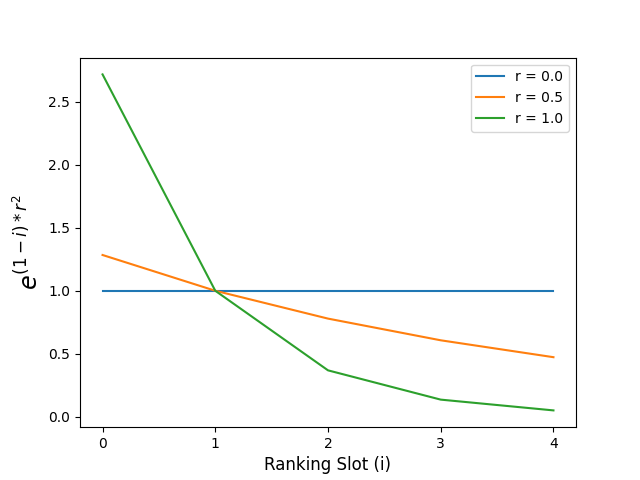
\includegraphics[width=0.7\textwidth]{images/ranking_factor.png}
	\caption{Effect of Ranking Factor}
	\label{ranking_factor_fig}
\end{figure}

\subsection{Ranked Bandits}

The Ranked Bandits algorithm \cite{radlinski2008learning} was developed by Radlinski et. al. in 2008. This was one of the first successful model for ranking search query results using reinforcement learning techniques. 

\textbf{Multi-Armed Bandits} is a classic reinforcement learning problem which deals with how to maximize the reward outcome in a given scenario based on the given choice of actions and the benefit/drawback associated with each making a choice only known partially to the algorithm. This is a typical explore-exploit scenario, where the agent wants to explore new choices in the action space for different scenarios, but also wants to have a conservative approach to maximize its rewards based on actions it takes. This balancing act is carried out in several different ways by different Multi-Armed Bandit algorithms.

Below we outline the steps taken by Ranked Bandits to train and ultimately provide a list $L_{v}$ for a given node $v$. 

\begin{enumerate}
	\item $k$ Multi-Armed Bandits $(MAB_{1},...,MAB_{k})$ are initialized for $k$ ranking slots. Each $MAB_{j}$ is responsible for suggestion of the node at the $j$-th index in $L_{v}$. The $MAB$s internally uses the Exp3 algorithm \cite{auer2002nonstochastic} for making an action choice (in this case choosing a node from the list of nodes in $V^{\prime}_{i}$). Exp3 was found to perform better by Radlinski et. al., and hence we choose the same for our purpose.
	
	\item At each training iteration, each $MAB_{j}$ is queried for the best node suggestion at index $j$ with reference to the seeking node $v$. The $MAB$s are queried in order, from $0$ to $k$. If $MAB_{j}$ suggests node $u_{j}$, then a check is made to see if this node was previously suggested by any other $MAB_{<j}$ for that training iteration. In case, that happens then a random node is chosen among the list of available nodes in $V^{\prime}_{i}$ and put as $u_{j}$.
	
	\item The recommendation list $L_{v}=(u_{1},..u_{k})$ is provided to the click model $C$, and a bitset $B=(b_{0},...,b_{k})$ is returned by $C$ where $b_{*}$ is either marked as 0 or 1, signifying whether the node was chosen by $C$ or not.
	
	\item If $u_{j}$ in $L_{v}$ was originally suggested by $MAB_{j}$ and $C$ chose it, then a reward of 1 is provided to the $MAB_{j}$ for suggesting that node. Else a reward of 0 is given to the $MAB_{j}$. With the reward values, the $MAB$s adjust their internal action specific gains which leads to better future predictions.
\end{enumerate}

\subsection{Top Rank}

Top Rank \cite{lattimore2018toprank} was developed by Lattimore et. al. in 2018. Earlier algorithms used to have mostly offline training mechanisms, whereas this was the first algorithm to make the learning process continuous (online learning). The basic idea of the algorithm is to maintain partial sets of nodes with preference ranking amongst these sets according to the feedback it receives by observing clicks. It keeps updating these partial set elements upon receiving feedback about them such that items in a higher set are always known to have better reward on selection. 

A broad overview of the steps taken by Top Rank is given below. 

\begin{enumerate}
	\item A partition set $P=\{P_{0}\}$ is initially created, where $P_{0}$ contains all nodes in $V^{\prime}_{i}$. 
	
	\item $k$ nodes are selected at each training iteration from the partitions in $P$. Partitions are ranked according to their index, so $P_{0}$ has a higher preference over $P_{1}$, which has higher preference over $P_{2}$, and so on. All nodes belonging to a certain partition have the same preference. A list $L_{v}=(u_{1},..u_{k} | u_{*} \in V^{\prime}_{i}(v))$ is created from the partitions in $P$, chosen according to precedence. Nodes from the same partition are always selected randomly, and the next partition is considered for node selection only when the previous one has been exhausted and the $L_{v}$ list still has less than $k$ nodes. 
	
	\item The $L_{v}$ list, upon creation, is provided to the click model $C$ which returns a bitset $B=(b_{0},...,b_{k})$ where $b_{*}$ is either 0 or 1, signifying whether the node at that position was chosen by $C$ or not.
	
	\item Using the feedback received from $C$ it is determined whether the existing partitions in $P$ can be broken down further based on the confidence of a node being placed in a higher preference partition or being demoted down to a lower partition. The details of the calculation which aids this decision can be found in the original paper \cite{lattimore2018toprank}.
	
	\item Steps 2-4 are repeated for all the training iterations. Finally we get the complete node set $V^{\prime}_{i}$ divided into partitions $P$ ranked according to preference.
	
	\item The Partition sets $P$ is used to get node recommendations in the same way as step 2 suggests.
	
\end{enumerate}

\section{Summary}

We end the chapter with a brief summary of all the recommendation methods which we would be using in the subsequent chapters and will be abstracting as $R$. We also introduce the short keyword names for the methods as \textbf{bolded text} here, which we use in the future chapters: in plots and discussions.

\textbf{PA-Homophily}: The preferential attachment with homophily method uses the probability measure in Karimi's generative model \cite{karimi2018homophily} for node rankings and recommendations.

\textbf{Adamic-Adar}: The Adamic-Adar Index uses an index measure as defined by Adamic et. al. \cite{adamic2003friends}. It recommends nodes based on similarity of nodes in terms of neighbours they share.

\textbf{Twitter-Rank}: Ranking used by Twitter to drive Who-To-Follow \cite{gupta2013wtf}. Combines SALSA scoring and egocentric random walk methods to get a recommendation list.

\textbf{Ranked-Bandit}: Reinforcement Learning method which maintains different MABs for each index in the recommendation list \cite{radlinski2008learning}. Each MAB is responsible to recommend the best node for that index. The MABs use Exp3 internally to perform the explore-exploit balance of choosing nodes among the given choice-set.

\textbf{Top-Rank}: Reinforcement Learning method which maintains several partitions, which are ordered according to preference and contains a partial ranking of all nodes \cite{lattimore2018toprank}. The partitions are updated or nodes are moved among them on the basis of observation of clicking behavior. 
% Chapter 4
\chapter{Analyzing Synthetic Data}
\label{analysis_chapter}
\thispagestyle{empty}

In this chapter we focus on our research goals \textbf{RG1.1} and \textbf{RG2} as defined in section \ref{research_goals}. This chapter is divided into two sections. We name the first section as \textbf{Static networks}, to signify working with pre-generated synthetic networks as per \textbf{RG1.1}. The next section is named as \textbf{Growing networks} to signify the growth of synthetic networks with the aid of recommendation engine ($R$) as per the requirement of \textbf{RG2}.

We start each section by defining the experimental setup for the given goal and how we strive to fulfill it. We define the algorithm we follow for the generation of synthetic networks which we would use for our analysis and also state the various static and tuneable parameters for our experiments. Once we have clearly defined our setup, we look at the results obtained through our experiments in the following subsections and analyze them in detail. We finish each section with the important findings from our observations.

\section{Static Networks}
\label{static_networks}
In this section we deal with pre-generated synthetic networks. In the experimental setup subsection we first talk about how we generate these pre-generated synthetic networks. In the results subsection we look at the different properties of these pre-generated synthetic networks and analyze the visibility bias we observe in the recommendation results.

\subsection{Experimental Setup}
We need to generate synthetic networks which can be used for our bias analysis. For the generation of synthetic networks we use the steps designed by Karimi et. al. \cite{karimi2018homophily}. Algorithm \ref{algo_karimi_model} shows the detailed steps we use to output a synthetic network $G_{t}(V_{t},E_{t})$ where $\delta(x)$ denotes the current degree of the node $x$ in the network. We then use these generated synthetic network as an input to generate a recommendations list ($L_{v}, |L_{v}|=k$) for each node $v \in V_t$. The recommendation list $L_{v}$ is given by the various recommender engines $R$ (the working of which we have discussed previously in detail in chapter \ref{recommender_methods}) we use.

\begin{algorithm}
	\SetAlgoLined
	\DontPrintSemicolon
	\SetKwInOut{Input}{input}\SetKwInOut{Output}{output}
	\Input{Total iterations : $t$\\Initial number of nodes : $m_{0}$\\Edges added per iteration: $m \leq m_{0}$\\Symmetric homophily value : $h$\\Minority Fraction: $f$}
	\Output{Network : $G_{t}(V_{t},E_{t})$ where $|V_{t}| = t+m_{0}, |E_{t}| \leq mt$}
	\BlankLine
	$n \leftarrow t+m_{0}$\;
	$N = \{v_{1},...,v_{n}\}$\;
	Assign $(f \times n)$ nodes in $N$ randomly to the minority group. Assign rest of the nodes in $N$ to the majority group.\;
	$V_{0} = \{v_{1},...,v_{m_{0}}\}$\;
	\For{$i \leftarrow 1$ \KwTo $t$}{
		$j \leftarrow (i+m_{0})$\;
		$V_{i} = V_{i-1} \cup \{v_{j}\}$\;
		\ForEach{vertex $u \in V_{i-1}$}{
			$\Pi_{u} = (\delta(u) \times h_{uv_{j}}) / \sum_{w \in V_{i-1}}^{} (\delta(w) \times h_{wv_{j}}) $\; 
		}
		Choose destination set $D \subseteq V_{i-1}, |D| \leq m$ based on probabilities $\Pi_{u \in V_{i-1}}$\; 
		$E_{i} = E_{i-1} \cup \{(v_{j}, u) | u \in D\}$\;
	}
	\caption{Barabási-Albert network generation model with homophily \cite{karimi2018homophily}}\label{algo_karimi_model}
\end{algorithm}

In table \ref{table_karimi_model} we list down the various tuneable and static parameters in our experimental setup for algorithm \ref{algo_karimi_model}.

\begin{table}[h]
	\centering
	\begin{tabular}{ |c|c| }
		\hline
		\textbf{Parameter} & \textbf{Value} \\
		\hline
		Total Iterations ($t$) & 998 \\
		Initial Number of Nodes ($m_{0}$) & 2 \\
		Edges added per iteration ($m$) & 2 \\
		Symmetric homophily value ($h$) & [0.0, 0.2, 0.5, 0.8, 1.0] \\
		Minority Fraction ($f$) & [0.1, 0.2, 0.3, 0.4, 0.5] \\
		\hline
	\end{tabular}
	\caption{Parameters for generation of synthetic networks as outlined by algorithm \ref{algo_karimi_model}}
	\label{table_karimi_model}
\end{table}

To obtain the recommendation list $L_{v}$ for a node $v \in V_{t}$ from the recommendation engine $R$ we provide as input $G_{t}(V_{t}, E_{t})$ and $v$ to $R$ and receive as output the list $L_{v}$. In table \ref{table_recommendation} we list down the various parameters used by the Recommender system $R$.

\begin{table}[h]
	\centering
	\begin{tabular}{ |c|c| }
		\hline
		\textbf{Parameter} & \textbf{Value} \\
		\hline
		Training Iterations ($T$) & 10000 \\
		Length of recommendation list ($k$) & 5 \\
		Ranking Factor ($r$) & [0.0, 0.5, 1.0] \\
		\hline
	\end{tabular}
	\caption{Parameters for recommendation engine $R$}
	\label{table_recommendation}
\end{table}

\subsection{Experimental Results}
Given the experimental setup as discussed above, we generate synthetic networks by tuning the different tuneable parameters generating 5 simulations for each variation. Below we look at the plots for degree distribution, degree growth, fraction of minorities holding total degree and top D\% degree rank to gain insights about these generated network. Our findings are similar to that of Karimi et. al. in \cite{karimi2018homophily}, and the differences can be attributed to our use of less iterations ($t$) to generate smaller networks and having less number of simulations (5) for each variation. Upon understanding the network structure we next look at the Disparate Visibility \cite{fabbri2020effect} measure for the recommendations we gather for all nodes in the network. 

\subsubsection{Degree Distribution}

\begin{figure}[h!]
	\centering
	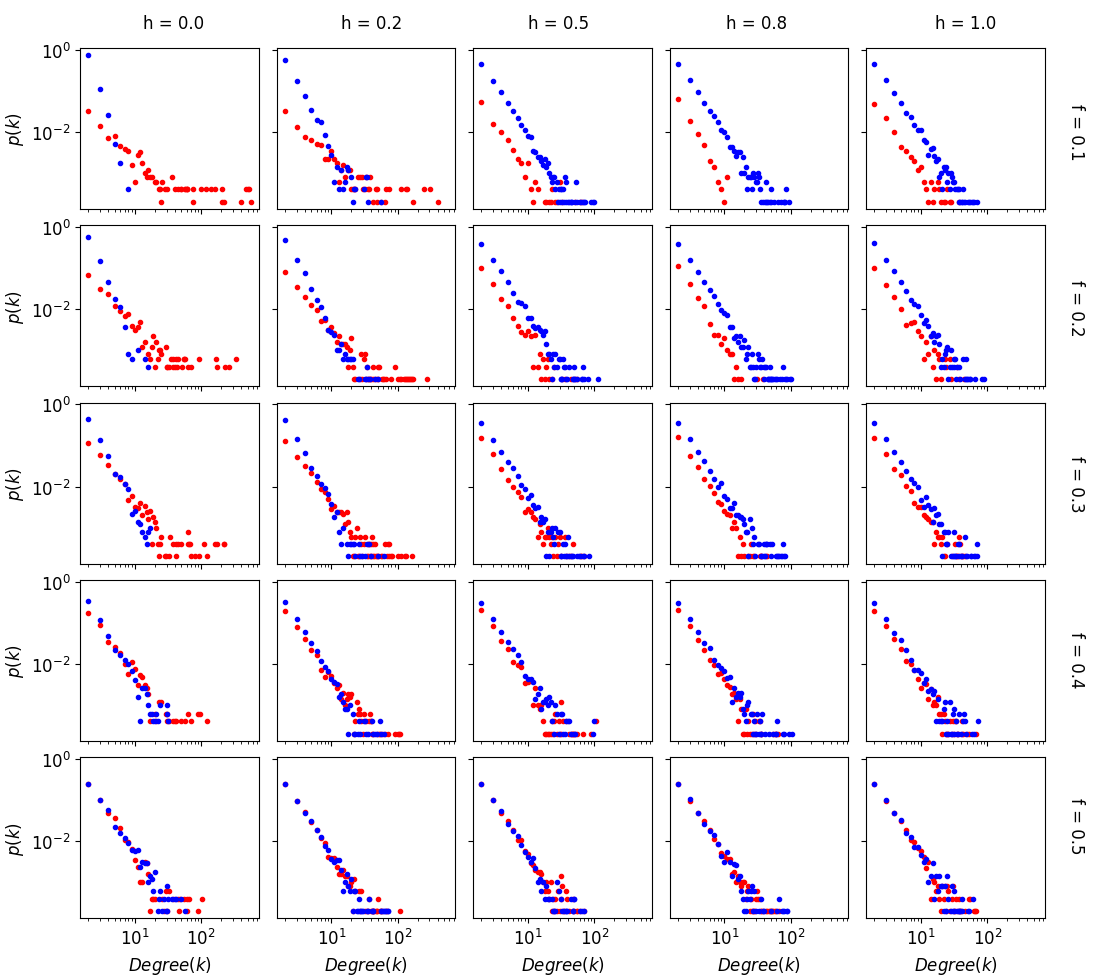
\includegraphics[width=1.0\textwidth]{images/dd_static.png}
	\caption{Degree distribution for static networks. The minority fractions are provided at the right-side of each row while the homophily is stated at the top of each column. Degree distribution for the majority and minority nodes are visualized using blue and red plot points respectively.}
	\label{dd_static_fig}
\end{figure}

Figure \ref{dd_static_fig} shows the plot for degree distribution of our generated synthetic networks. At the bottom row where both group sizes are same, the distribution is similar for all homophily values. As we go upwards towards networks with smaller minority group size, we see the disparity in distribution grow. Minority nodes are at an advantage in the heterophilic regime since they garner a lot of attention from the majority group. This changes as the homophily value increases putting majorities in favour as they prefer nodes from their own larger group. In a completely homophilic network, there exists in-group competition which decreases the difference in degree distribution values among groups.

\subsubsection{Degree Growth}

\begin{figure}[h!]
	\centering
	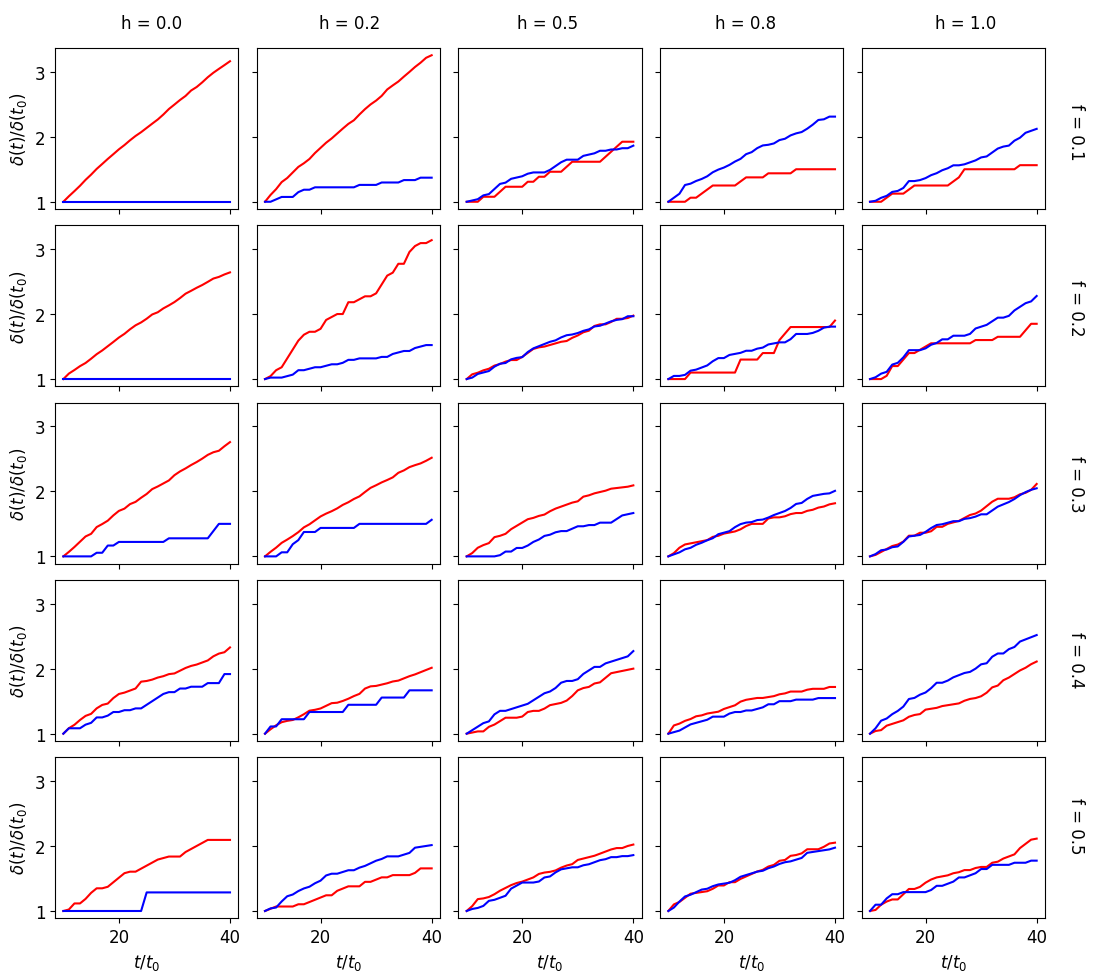
\includegraphics[width=1.0\textwidth]{images/dg_static.png}
	\caption{Degree growth for static networks. The minority fractions are provided at the right-side of each row while the homophily is stated at the top of each column. Degree growth for minority and majority node is visualized using the red and the blue color plot lines respectively.}
	\label{dg_static_fig}
\end{figure}

Figure \ref{dg_static_fig} shows how the degree of a majority and a minority node grows over time in the network generation process. We have realized before in our analysis of degree distribution, when the minority group size is small they tend to have higher degrees in heterophilic regime. In the homophilic regime, the majority groups have a slight advantage but due to competition amongst themselves this growth factor is small. We see in our plot however that when both group sizes are same, the minority has a higher growth over majority for $h=1.0$ and also the majority has a higher growth over minority at $h=0.8$. This is probably due to the choice of the nodes which contribute to the growth plot. We conducted similar network generation experiments for higher iteration values($t=5000$) and there we did not perceive this effect. We choose to keep these results though since these are the same networks we use in our later experiments. 

\subsubsection{Fraction of total degree held by minorities}

\begin{figure}[h!]
	\centering
	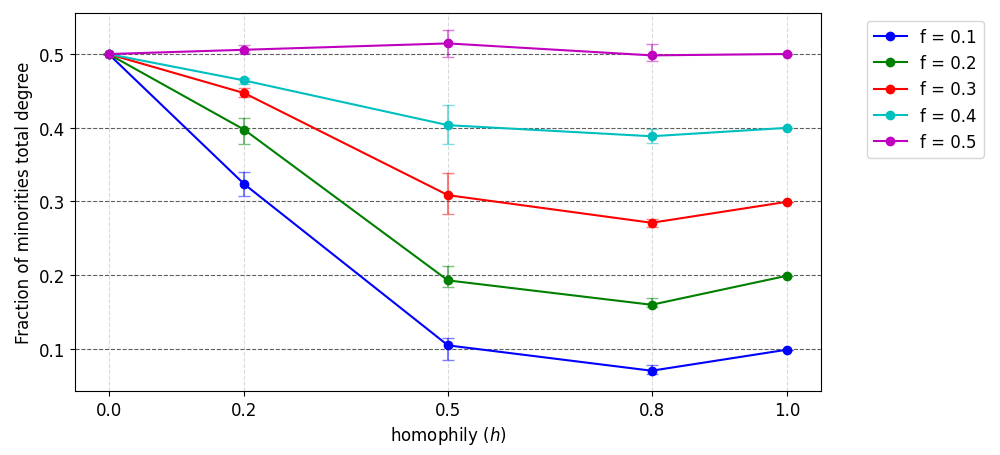
\includegraphics[width=0.8\textwidth]{images/mf_static.png}
	\caption{Fraction of total degree held by minority nodes in static networks at different minority fractions and different homophily values.}
	\label{mf_static_fig}
\end{figure}

Figure \ref{mf_static_fig} shows the fraction of total degrees held by the minority nodes in the network. In the heterophilic regime, the minority nodes hold a higher degree due to being favored by the majority nodes (which causes the \textit{``majority illusion''} problem). At $h=0.5$, where homophily doesn't play a role the degree fraction is nearly the same as minority group size. As we move towards the homophilic regime, the majority nodes do hold greater degree share at $h=0.8$ but this equalizes again as we near the complete homophily stage where the in-group support keeps both groups at appropriate degree share. 

\subsubsection{Top D\% degree rank}

\begin{figure}[h!]
	\centering
	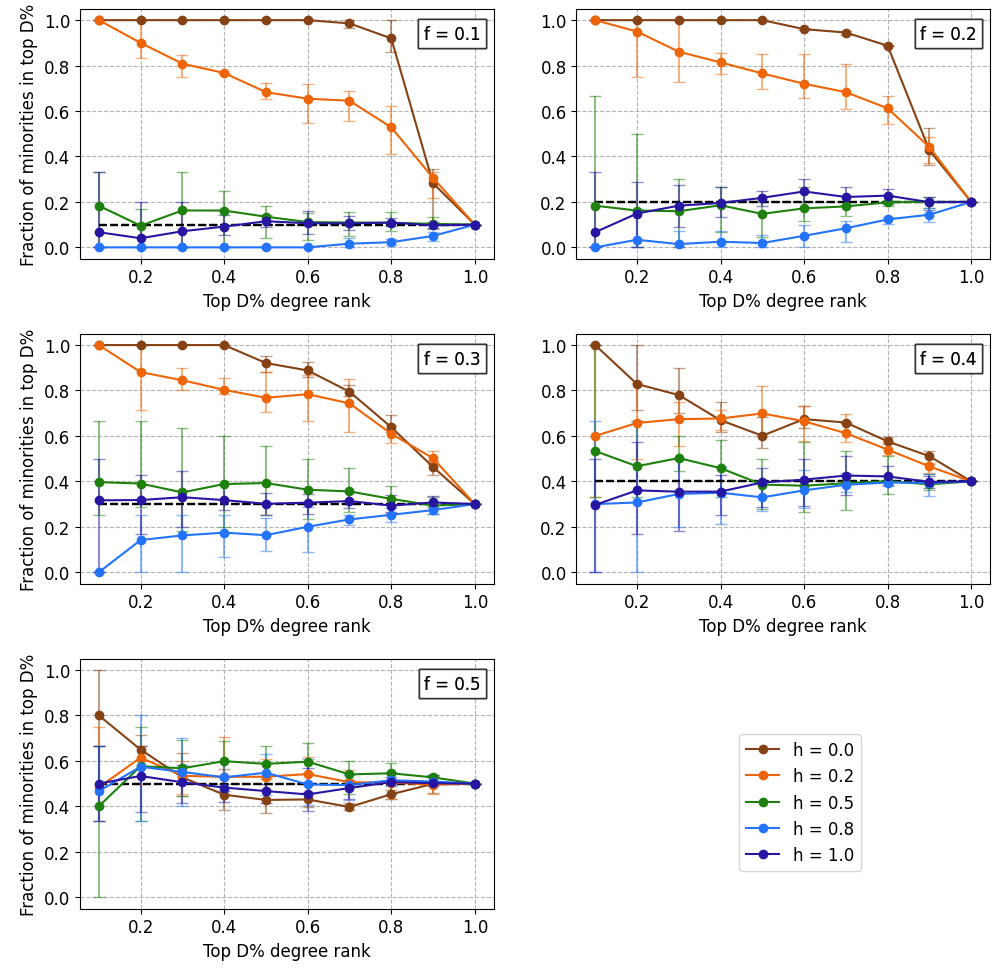
\includegraphics[width=1.0\textwidth]{images/top_static.png}
	\caption{The fraction of minority nodes found in top D\% nodes ranked according to degree in static networks. A black dotted line at each plot shows the actual fraction of minority nodes in the network.}
	\label{top_static_fig}
\end{figure}

Figure \ref{top_static_fig} shows the fraction of minority nodes which are present in the top D\% of node rankings (ranked according to degree). In heterophilic regime, the minority is highly over-represented than its group size, when the minority group size is small. This effect can be seen to reduce as the minority group size increases and the ranking at each percentage is closer to the original group size. At an equal group size, we can see that the degree rankings at each percentage adheres to the original group size.

\subsubsection{Disparate Visibility}
\label{static_dv}

\begin{figure}[h!]
	\centering
	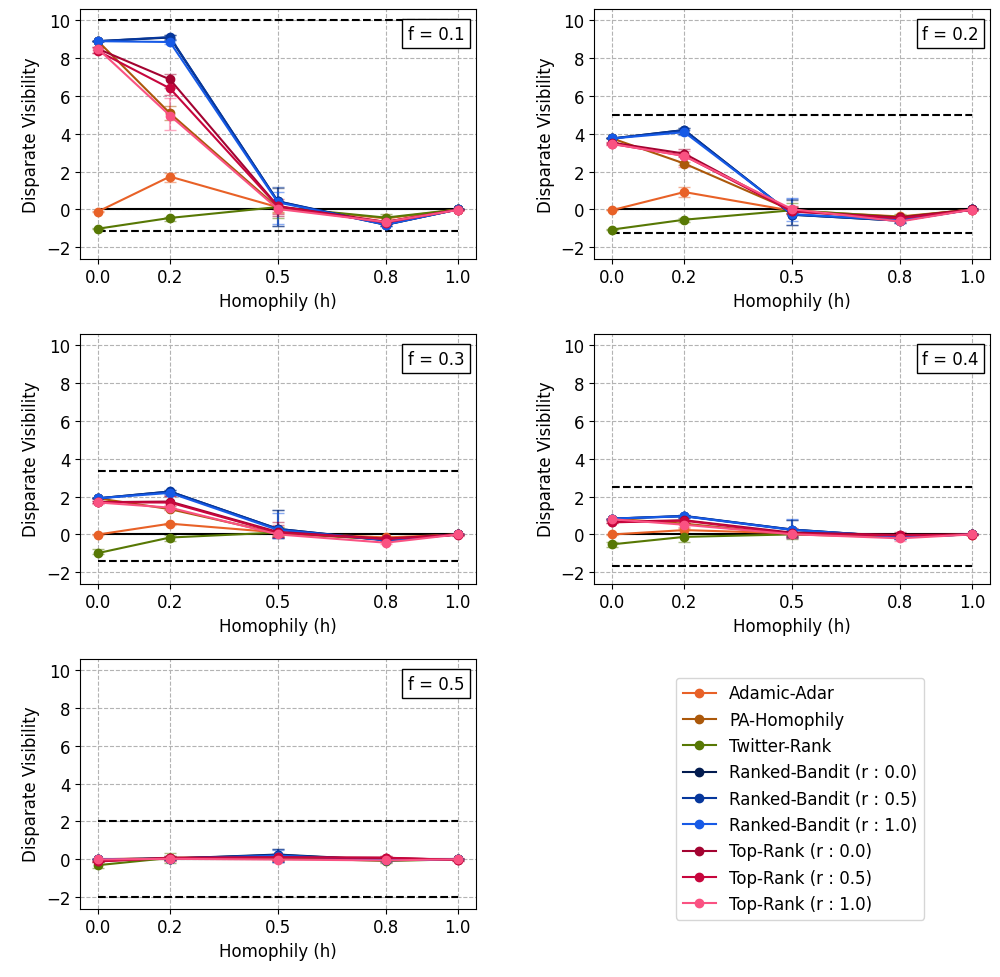
\includegraphics[width=1.0\textwidth]{images/dv_static.png}
	\caption{Disparate Visibility measure for static networks of different minority group sizes. The black line at each plot shows the equal visibility point and the black dotted lines represent the upper and lower limit for the disparate visibility measure.}
	\label{dv_static_fig}
\end{figure}

Figure \ref{dv_static_fig} shows the disparate visibility measure for the various recommendation methods. In the heterophilic regime we can see that minority nodes gain much higher visibility in recommendations for the \textbf{reinforcement methods} and \textbf{PA-Homophily} method. This we can expect as in the heterophilic regime the minorities are highly over-represented since they are likely to connect with the large number of majorities. As the minority fraction increases, this effect is seen to reduce. In the homophilic regime, although we see slight visibility gain for majority nodes at $h=0.8$ this is not that significant. The values lie quite close to equal visibility in recommendations at the homophilic regime.

For the \textbf{Adamic-Adar} and \textbf{Twitter-Rank} methods we observe a close stable measure with almost equal visibility for both groups at all homophily cases. 

For Adamic-Adar at $h=0$ we observe that the disparate visibility is always 0. This happens because in the case of complete heterophily, for Adamic-Adar, minority nodes are always suggested minority nodes and majority nodes are always suggested majority nodes. This happens owing to how the Adamic-Adar method works internally. To elaborate our point, we can consider the bipartite graph $G_t$ at $h=0$ as input to our recommender $R$ driven by Adamic-Adar. We know that Adamic-Adar suggests nodes based on common neighbours. Two minority nodes in $G_t$ would only have majority nodes in common at $h=0$ and thus a minority node would only be recommended to minorities. This same logic also holds in the case of a majority node recommendations. Thus, the disparate visibility is always at 0 in the case of complete heterophily for Adamic-Adar.

In the case of Twitter-Rank also we notice balanced visibility for both groups. While for Adamic-Adar we see from the plots that although there is equal visibility at $h=0$, the visibility for minorities is quite high at $h=0.2$. For Twitter-Rank however we can see that the visibility measure is quite near to the equal visibility line at all homophilies. 

\subsection{Summarized Findings}

We list down our observations from the experiments on Static Networks below.

\begin{enumerate}
	\item In the heterophilic regime, minority group nodes are at an advantage. In the homophilic regime, majority group nodes do tend to gain some advantage, but due to fierce competition amongst themselves this is very slight.
	
	\item As the minority group size increases and it gets closer to the equal group-size ($f=0.5$), the minorities start losing advantage over the majority in heterophilic regime. This phenomenon is also true for the majorities in the homophilic regime.
	
	\item The bias in recommendations received with different recommendation systems are highest in the case of \textbf{reinforcement methods} and \textbf{PA-Homophily} at the heterophilic regime. In the homophilic regime the visibility is close to equal for both groups. \textbf{Twitter-Rank} provides best equality in visibility for both groups in recommendations, also closely followed by \textbf{Adamic-Adar}.
	
\end{enumerate}

\section{Growing Networks}
\label{growing_networks}
In this section we propagate growth of synthetic networks, in which the growth is influenced by the use of different recommender systems $R$. In the experimental setup sub-section we lay down the detailed algorithm which we use for growing these networks. In the results sub-section we look in detail at the different properties of these recommendation influenced networks.

\subsection{Experimental Setup}
We generate our network by using algorithm \ref{growing_network_model}. We take influence from the \textit{recommendation algorithm model} by Stoica et. al. \cite{stoica2018algorithmic} while developing our growth algorithm. The key difference between the two approaches is the usage of a generic recommendation engine $R$ in our case and the usage of the karimi model \cite{karimi2018homophily} to make edge-formation decisions. 

\begin{algorithm}
	\SetAlgoLined
	\DontPrintSemicolon
	\SetKwInOut{Input}{input}\SetKwInOut{Output}{output}
	\Input{Total iterations : $t$\\Symmetric homophily value : $h$\\Probability of node being marked as minority node: $f$\\Recommender Engine : $R$\\Organic Growth Probability : $\alpha$\\Randomness : $\mu$\\Number of recommendations : $k$\\}
	\Output{Network : $G_{t}(V_{t},E_{t})$}
	\BlankLine
	With probability $f$ mark node $v_{0}$ as minority, else mark as majority.\;
	$V_{0} = \{v_{0}\}$\;
	\For{$i \leftarrow 1$ \KwTo $t$}{
		With $\alpha$ probability, choose $growth\_type$ as $organic$, else choose $algorithmic$.\;
		\uIf{$growth\_type$ is $organic$}{
			$V_{i} = V_{i-1} \cup \{v_{i}\}$\;
			With probability $f$ mark node $v_{i}$ as minority, else mark as majority.\;
			With probability $\mu$ choose $random\_connect$ as true, else choose false.\;
			\eIf{$random\_connect$ is true}{
				Choose node $u_{i}$ from $V_{i-1}$ at random.\;
			}{
				\ForEach{vertex $u \in V_{i-1}$}{
					$\Pi_{u} = (\delta(u) \times h_{uv_{i}}) / \sum_{w \in V_{i-1}}^{} (\delta(w) \times h_{wv_{i}}) $\; 
				}
				Choose $u_{i}$ based on probability $\Pi_{u \in V_{i-1}}$\;
			}
		}
		\ElseIf{$growth\_type$ is $algorithmic$}{
			$V_{i} = V_{i-1}$\;
			Choose $v_{i}$ from $V_{i}$ at random.\;
			Get recommendation list $L_{v_{i}} (|L_{v_{i}}|=k)$ for $v_{i}$ from recommender engine $R$.\;
			\ForEach{vertex $u \in L_{v_{i}}$}{
				$\Pi_{u} = (\delta(u) \times h_{uv_{i}}) / \sum_{w \in L_{v_{i}}}^{} (\delta(w) \times h_{wv_{i}}) $\; 
			}
			Choose $u_{i}$ based on probability $\Pi_{u \in L_{v_{i}}}$.\;
		}
		\eIf{$u_{i}$}{
			$E_{i} = E_{i-1} \cup \{(u_{i},v_{i})\}$\;
		}{
			$E_{i} = E_{i-1}$\;	
		}
	}
	\caption{Growing network model}\label{growing_network_model}
\end{algorithm}

In table \ref{table_growth_model} we list down the various tuneable and static parameters in our experimental setup for algorithm \ref{growing_network_model}. As the recommendation engine $R$, we use the following methods: PA-Homophily, Adamic-Adar, Twitter-Rank, Ranked-Bandit, Top-Rank (which we have discussed in detail in chapter \ref{recommender_methods}). The additional parameters used by the reinforcement methods are the same as listed in table \ref{table_recommendation}.

\begin{table}[h]
	\centering
	\begin{tabular}{ |c|c| }
		\hline
		\textbf{Parameter} & \textbf{Value} \\
		\hline
		Total iterations ($t$) & 10000 \\
		Randomness ($\mu$) & 0.1 \\
		Organic growth probability ($\alpha$) & 0.1 \\
		Symmetric homophily value ($h$) & [0.0, 0.2, 0.5, 0.8, 1.0] \\
		Probability of minority node ($f$) & [0.1, 0.2, 0.3, 0.4, 0.5] \\
		Number of recommendations ($k$) & 5 \\
		Recommender training iterations ($T$) & 10000 \\
		Ranking factor ($r$) & [0.0, 0.5, 1.0] \\
		\hline
	\end{tabular}
	\caption{Parameters for generation of synthetic networks as outlined by algorithm \ref{growing_network_model}}
	\label{table_growth_model}
\end{table}

What we can observe from our algorithm given the experimental setup is that the synthetic networks which we receive as output would be having more number of edges than the previous synthetic networks used in section \ref{static_networks} owing to \textit{algorithmic growth}. The total number of iterations for the generation of $G_{t}$ is $t=10000$. Given the organic growth probability $\alpha=0.1$, we expect the total number of nodes $|V_{t}| \simeq 1000$. Since the number of edges are quite high, owing to \textit{algorithmic growth}, the average degree of nodes also increases, which can be seen very specifically in some plots (specially that of \textit{Adamic-Adar}). Also another notable difference with the networks generated in section \ref{static_networks} is that $h=0$ may not mean a completely bipartite graph in the case of \textit{growing networks} since there is a randomness factor $(\mu)$ at play here. Also by similar logic, for a value of $h=1$ the synthetic network might not be completely disjoint. How all these factors come together and influence the network growth we will be seeing in the next few sections.

Now that we have detailed the experimental setup, we generate synthetic networks by tuning the different parameters in table \ref{table_growth_model}, having 5 simulations for each variation. In the subsequent sections we list the various results for our experiments and also our analysis for them. 

\subsection{Experimental Results : PA-Homophily}

\begin{figure}[h!]
	\centering
	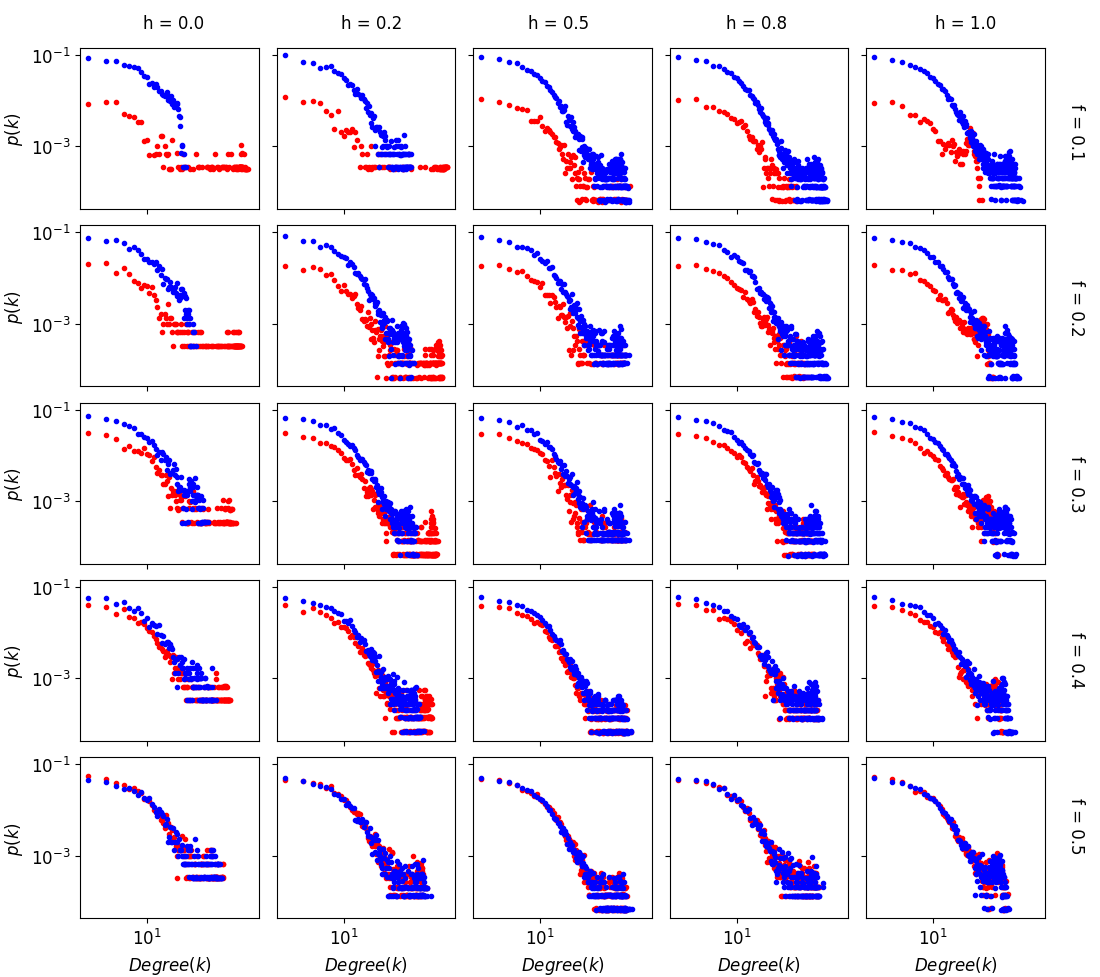
\includegraphics[width=1.0\textwidth]{images/dd_growth_pa.png}
	\caption{Degree distribution for growing networks with \textbf{PA-Homophily}. The minority fractions are provided at the right-side of each row and the homophily values are specified at the top of each column. Degree distribution for the majority and minority nodes are visualized using blue and red plot points respectively.}
	\label{dd_growth_pa_fig}
\end{figure}

\begin{figure}[h!]
	\centering
	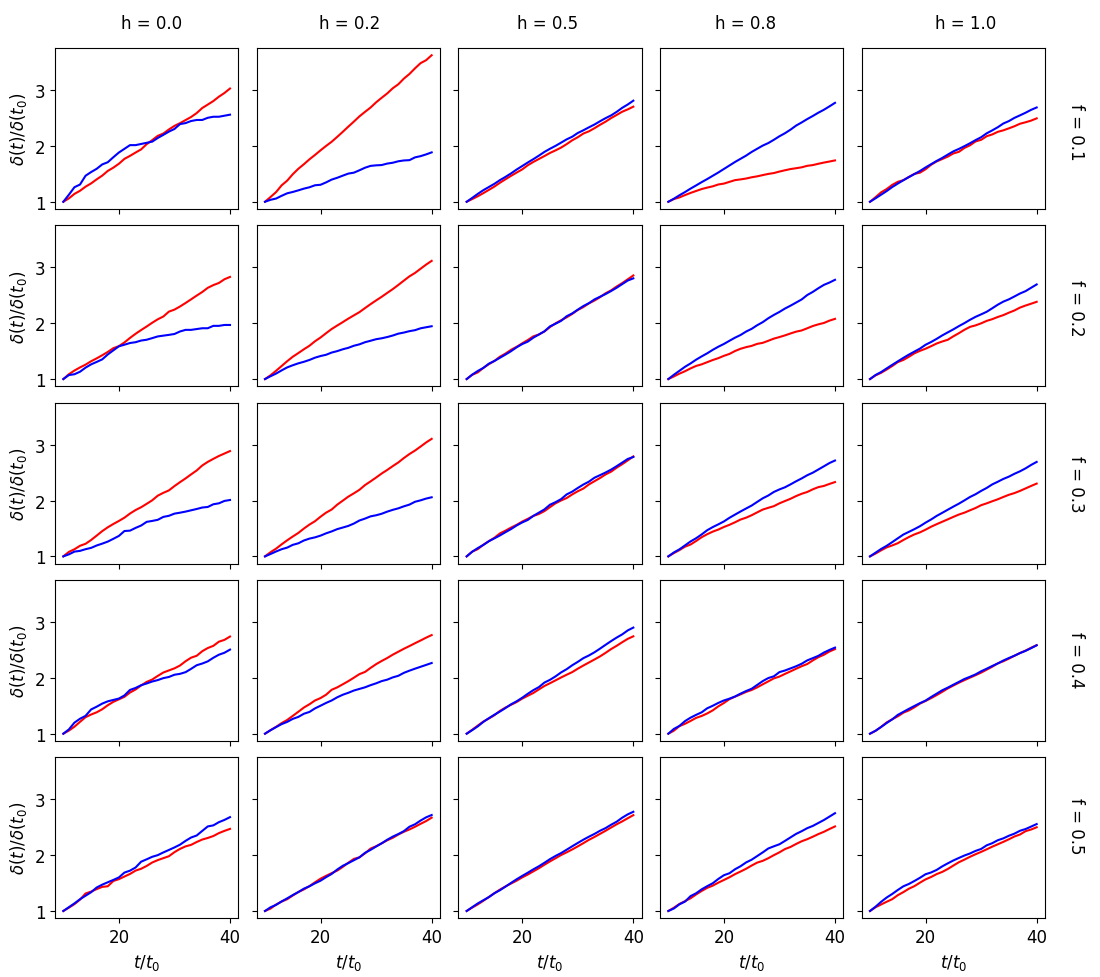
\includegraphics[width=1.0\textwidth]{images/dg_growth_pa.png}
	\caption{Degree growth for growing networks with \textbf{PA-Homophily}. The minority fractions are provided at the right-side of each row and the homophily values are specified at the top of each column. Degree growth for minority and majority node is visualized using red and blue color plot lines respectively.}
	\label{dg_growth_pa_fig}
\end{figure}

\begin{SCfigure}[1][h!]
	\centering
	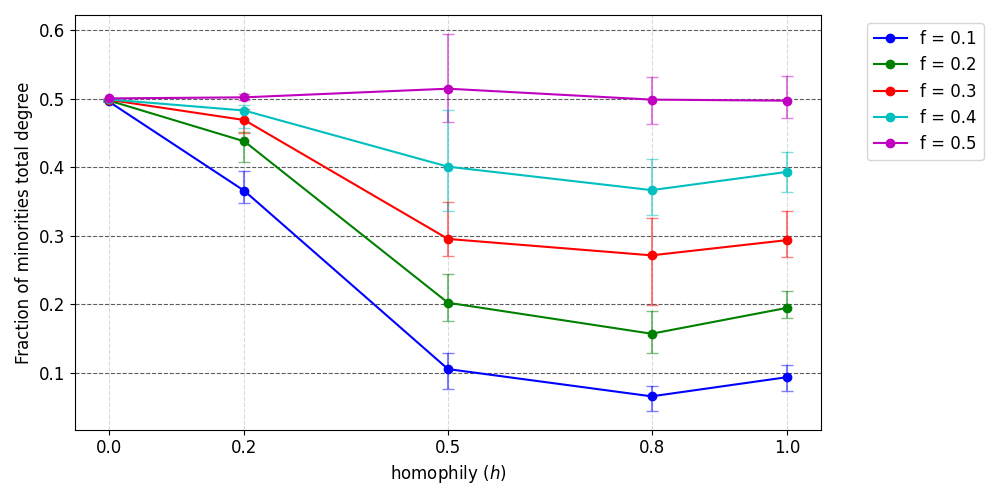
\includegraphics[trim=0 5 0 10, clip, width=0.75\textwidth]{images/mf_growth_pa.png}
	\caption{The fraction of total degree held by minority nodes for growing networks with \textbf{PA-Homophily}.}
	\label{mf_growth_pa_fig}
\end{SCfigure}

\begin{figure}[h!]
	\centering
	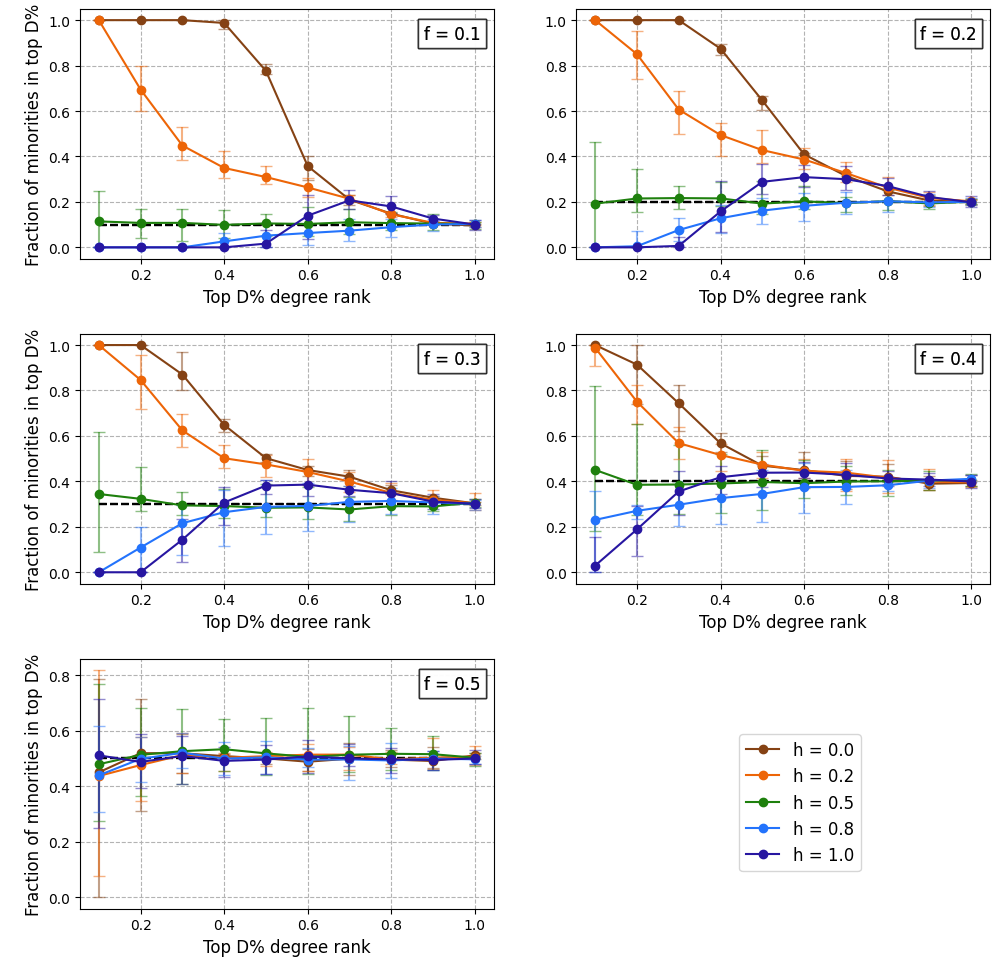
\includegraphics[trim=0 10 0 5, clip, width=1.0\textwidth]{images/top_growth_pa.png}
	\caption{The fraction of minority nodes found in top D\% nodes ranked according to degree in growing networks with \textbf{PA-Homophily}. A black dotted line at each plot shows the actual fraction of minority nodes in the network.}
	\label{top_growth_pa_fig}
\end{figure}

In the case of \textit{PA-Homophily}, the recommender method calculates probability of candidate nodes to be chosen for connection with seeking node by considering parameters like degree of the candidate nodes and homophily between the candidate and the seeking node.

In the \textbf{heterophilic} regime, we can see that the minority nodes have a clear edge over majority nodes and this is higher in case of lower minority group sizes. The large number of majority nodes in this regime choose to give attention to the fewer minority nodes which lead to these minorities ultimately holding higher degrees. This can be seen from the degree distribution plot (figure \ref{dd_growth_pa_fig}).

From the degree growth plot (\ref{dg_growth_pa_fig}) we can see that minorities would have higher degree growth than majorities due to this attention from majorities. They also hold very high amount of the total degree in the networks as can be seen in figure \ref{mf_growth_pa_fig}. This clearly shows that the minorities are having a high over-representation in this regime. Ranking the nodes according to their degrees confirms this for us as we can see in figure \ref{top_growth_pa_fig} that the top rank holders are mostly minority nodes. The recommendation lists for minorities and majorities have nodes from the other groups highly and thus driven by the algorithmic growth this gives us a network similar to what we get from the models generated by algorithm \ref{algo_karimi_model} in the case of \textit{static networks}.

In the \textbf{homophilic} regime, from the degree distribution plot (figure \ref{dd_growth_pa_fig}) we see that majorities tend to hold higher degrees than minorities which is expected since the groups tends tend to connect amongst themselves and the majorities are larger in number.

We also see that the minority nodes are recommended a lot more majority nodes in their recommendation lists, specially when the minority size is very low and homophily is $h=0.8$. At $h=0.8$, the majority has higher growth but the difference with growth of minorities is not very high.

At complete homophily only in-group support is present so then the reversed effect of $h=0$ can be seen for lower minority fractions. Looking at the plot in figure \ref{mf_growth_pa_fig} we can see that the minorities share of total degrees is only slightly lower than its group size at $h=0.8$. Ranking these nodes according to degree as done in figure \ref{top_growth_pa_fig} shows that minorities are underrepresented. At $h=1$ we see that the minorities tend to be over-represented at about the $D=40\%$ mark. We saw this effect slightly before in our pre-generated synthetic networks in figure \ref{top_static_fig}. We have confirmed that this effect is not seen for networks with about 5000 nodes and we believe that this is only seen due to the less number of nodes we use in our networks. Also, the randomness factor ($\mu$) adds an extra exaggeration to this effect which might be another factor to cause this kind of over-representation for our plots in the \textit{growing networks} perspective.

\subsection{Experimental Results : Adamic-Adar}

In the case of \textit{Adamic-Adar}, the growth is completely based on the network structure that develops over time. The recommendation system is agnostic of the type of nodes it is dealing with when recommending and is solely dependent on the neighbours of the seeker and candidate nodes used to calculate the Adamic-Adar index. 

\begin{figure}[h!]
	\centering
	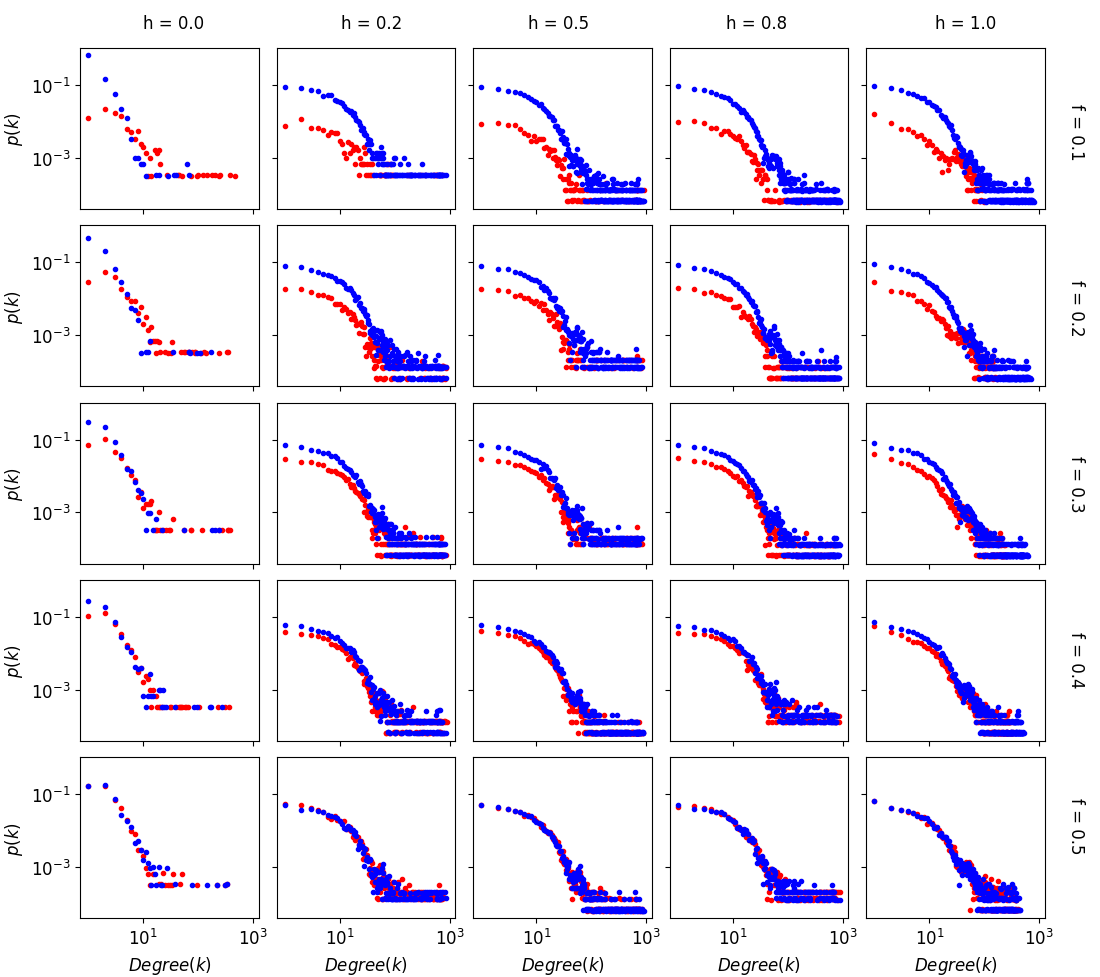
\includegraphics[width=1.0\textwidth]{images/dd_growth_aa.png}
	\caption{Degree distribution for growing networks with \textbf{Adamic-Adar}. The minority fractions are provided at the right-side of each row and the homophily values are specified at the top of each column.  Degree distribution for the majority and minority nodes are visualized using blue and red plot points respectively.}
	\label{dd_growth_aa_fig}
\end{figure}

\begin{figure}[h!]
	\centering
	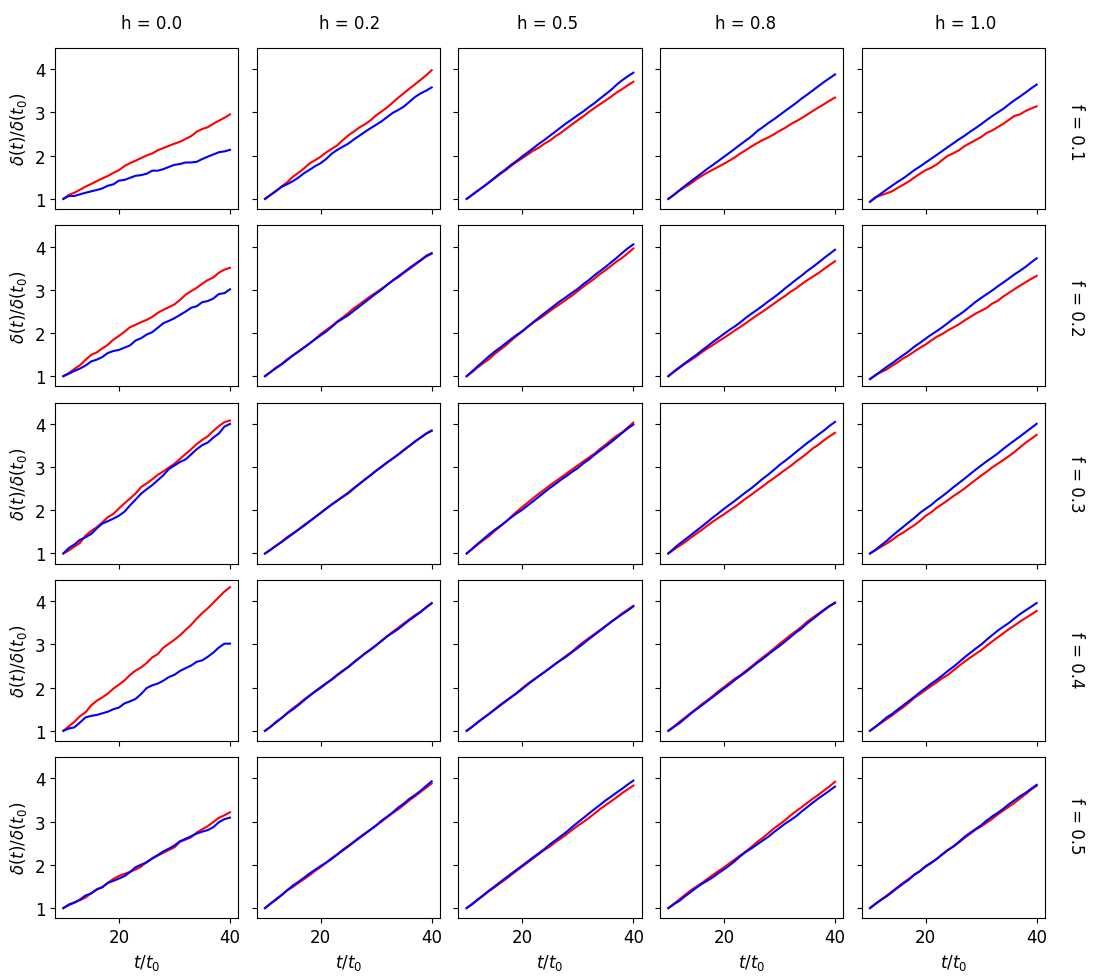
\includegraphics[width=1.0\textwidth]{images/dg_growth_aa.png}
	\caption{Degree growth for growing networks with \textbf{Adamic-Adar}. The minority fractions are provided at the right-side of each row and the homophily values are specified at the top of each column. Degree growth for minority and majority node is visualized using red and blue color plot lines respectively.}
	\label{dg_growth_aa_fig}
\end{figure}

\begin{SCfigure}[1][h!]
	\centering
	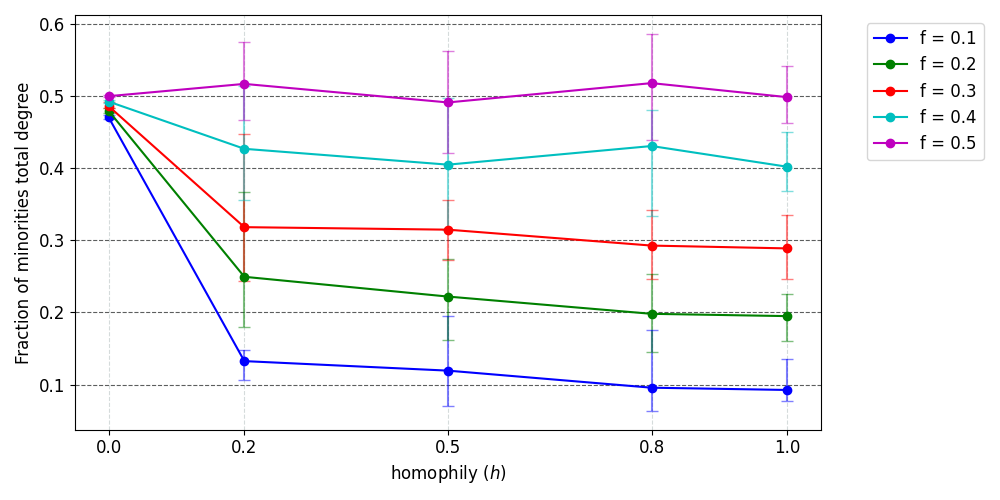
\includegraphics[trim=0 5 0 10, clip, width=0.75\textwidth]{images/mf_growth_aa.png}
	\caption{The fraction of total degree held by minority nodes for growing networks with \textbf{Adamic-Adar}.}
	\label{mf_growth_aa_fig}
\end{SCfigure}

\begin{figure}[h!]
	\centering
	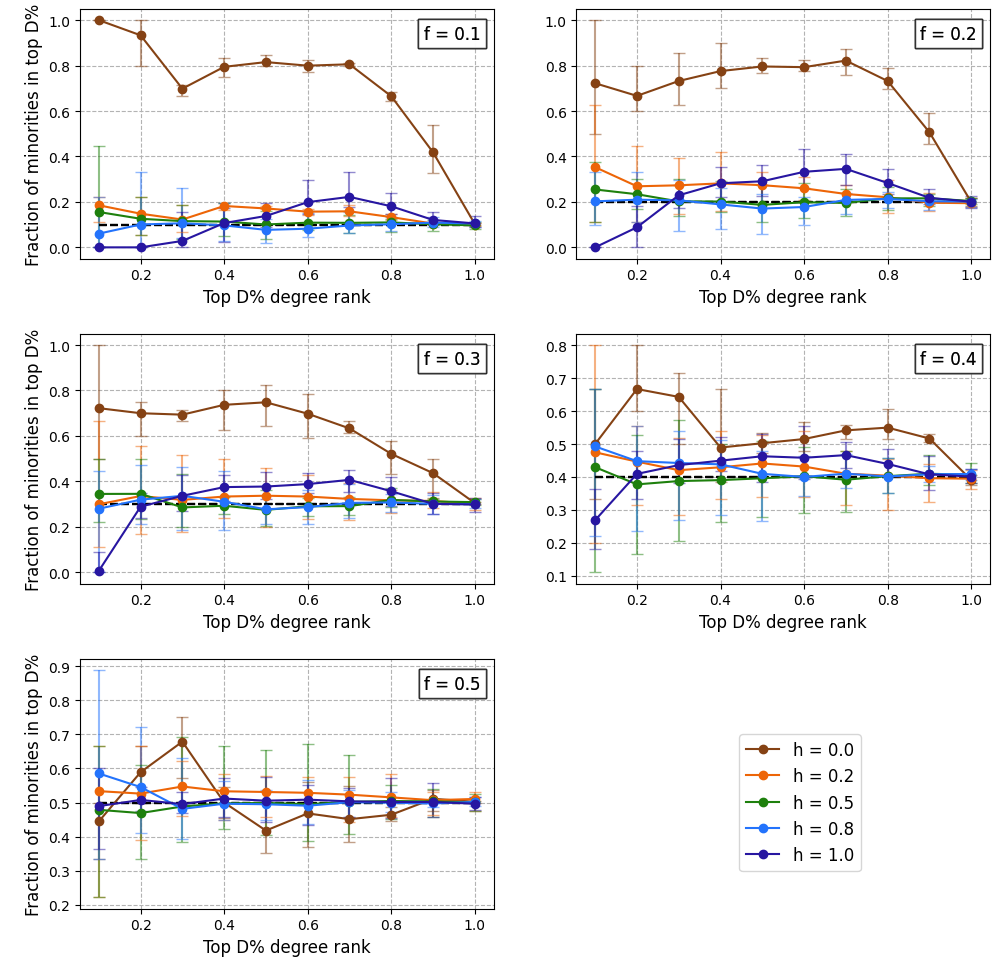
\includegraphics[trim=0 10 0 5, clip, width=1.0\textwidth]{images/top_growth_aa.png}
	\caption{The fraction of minority nodes found in top D\% nodes ranked according to degree in growing networks with \textbf{Adamic-Adar}. A black dotted line at each plot shows the actual fraction of minority nodes in the network.}
	\label{top_growth_aa_fig}
\end{figure}

Let us consider the \textbf{heterophilic} regime, where nodes prefer to get connected with nodes from the opposite group. In the extreme heterophilic case, nodes simply reject connection with nodes from the other group. If we consider homophily value of $h=0$, the nodes from same group which are suggested would be completely rejected for connections thus most of the recommendations would not result in any fruitful connections. However at $h=0.2$, even with weak probability they would connect which helps evolve the structure of the network unbiased. This difference between behavior at the two homophily values causes a stark difference in the degree distribution plot (figure \ref{dd_growth_aa_fig}) for Adamic-Adar. 

Also in the degree distribution plot (figure \ref{dd_growth_aa_fig}) we see that while at the extreme heterophily case ($h=0$), minority nodes do hold higher degrees in most cases, but with the change in minority group size there is not much change. It can be seen that the probability of having a lower degree minority node seems to be increasing with the increase in minority group size.

The degree growth plot (figure \ref{dg_growth_aa_fig}) shows that at $h=0$ homophily there is a slightly higher degree growth for the minorities which mostly happens due to the organic growth of the network. As the strict heterophily is relaxed and minorities start connecting with majorities even with weaker probabilities, we can see that both the minorities and majorities have high degree growth with time.

This can be further verified by checking the fraction of total degrees held by minority nodes (figure \ref{mf_growth_aa_fig}) where at $h=0.2$ we see that the minorities hold degree close to its original size. Also with the degree ranking plot (figure \ref{top_growth_aa_fig}) it is seen that the plot lines lie close to the fraction of minorities in the network at $h=0.2$ which signifies a balanced network. At $h=0$ we do see over-representation but that is only due to the strict heterophily measure and with even the slightest lax network would ease up towards the unbiased structure. 

In the \textbf{homophilic} regime, at $h=0.8$ there is high recommendation of majorities for both the minority and majority seeker nodes. The lesser the minority size the more majority nodes are recommended by the recommender. This is what aides the majorities to gain very high degrees compared to minorities in the case of $h=0.8$.

At $h=1$, majorities start getting recommended majorities and minorities start getting recommended minorities. This causes the minority nodes to also gain higher degrees like majorities and thus have similar distribution as can be seen in figure \ref{dd_growth_aa_fig}. Looking at the degree growth plot (figure \ref{dg_growth_aa_fig}) we see that both type of nodes have high degree growth with the majorities maybe slightly leading in the case of lower minority fractions. Since the degree of both type of nodes have similar growth we can also see that the fraction of total degrees held by both type of nodes is almost balanced according to the minority fraction of the network. This signifies that the minorities have almost the same representation as their group-size in degree ranking which can be seen in figure \ref{top_growth_aa_fig}.

The observation which we can draw from the Adamic-Adar recommendations is that the type of recommended nodes which the seeker nodes receive is almost similar at the extreme cases of homophily and heterophily. This harms in edge-connection in $h=0$ but helps in $h=1$. For the in-between cases there is always higher number of majority nodes recommended for both type of nodes which causes the visibility of the majorities to be at par with its group size.

\subsection{Experimental Results : Twitter-Rank}

\textbf{Twitter-Rank} bases ranking on the SALSA scoring mechanism. The nodes in hubs and authorities are formed by collecting nodes to form a ``circle of trust'' (hub side) and the nodes connecting  to the hubs (authorities side) which are then ranked according to the SALSA scores and provided as recommendations.

\begin{figure}[h!]
	\centering
	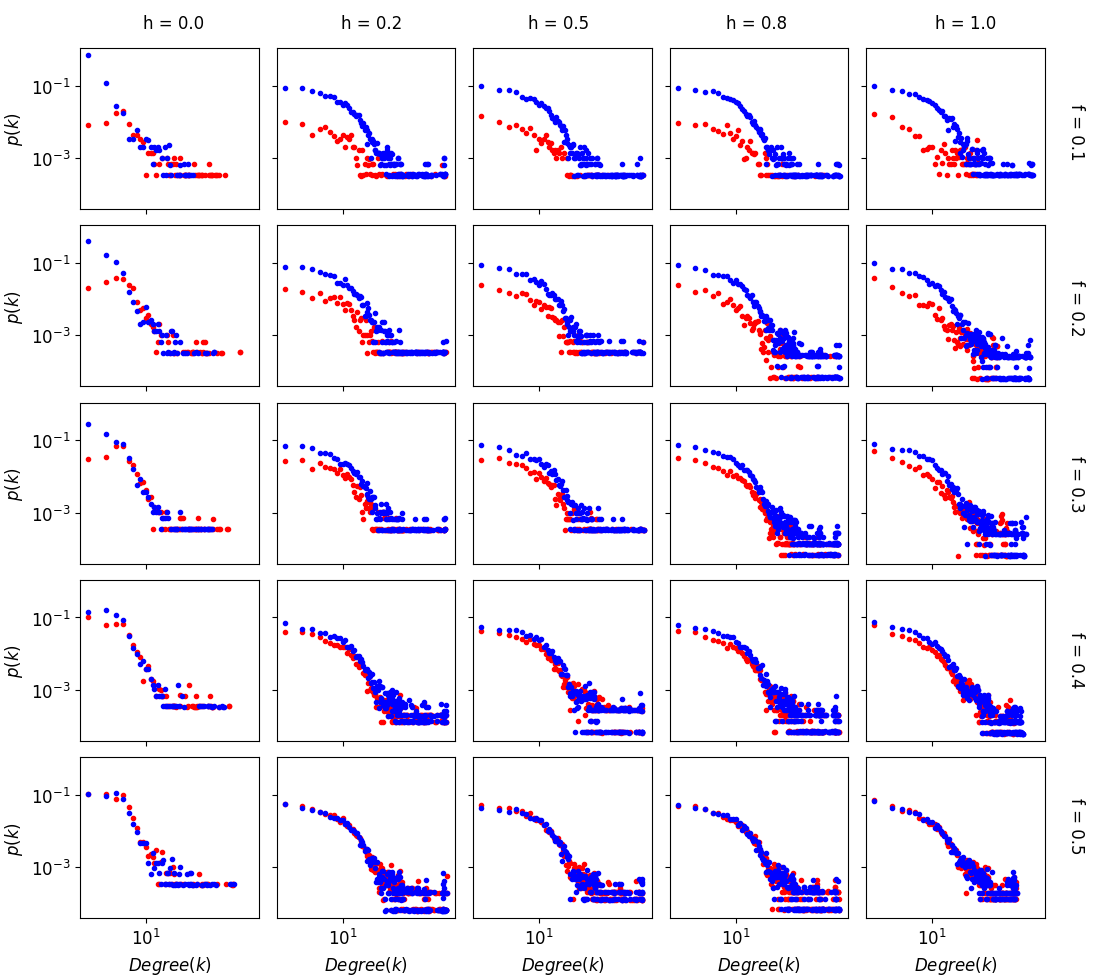
\includegraphics[width=1.0\textwidth]{images/dd_growth_tr.png}
	\caption{Degree distribution for growing networks with \textbf{Twitter-Rank}. The minority fractions are provided at the right-side of each row and the homophily values are specified at the top of each column. Degree distribution for the majority and minority nodes are visualized using blue and red plot points respectively.}
	\label{dd_growth_tr_fig}
\end{figure}

\begin{figure}[h!]
	\centering
	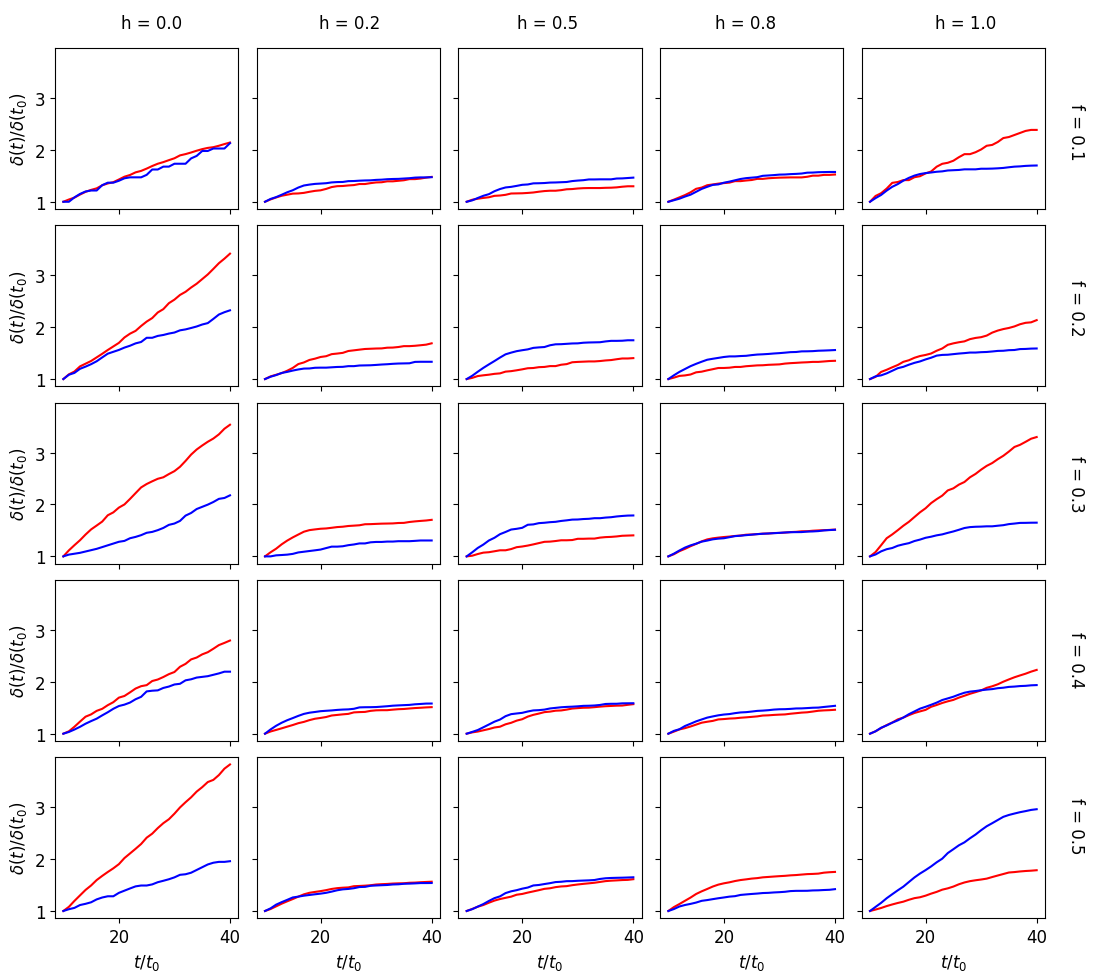
\includegraphics[width=1.0\textwidth]{images/dg_growth_tr.png}
	\caption{Degree growth for growing networks with \textbf{Twitter-Rank}. The minority fractions are provided at the right-side of each row and the homophily values are specified at the top of each column. Degree growth for minority and majority node is visualized using red and blue color plot lines respectively.}
	\label{dg_growth_tr_fig}
\end{figure}

\begin{SCfigure}[1][h!]
	\centering
	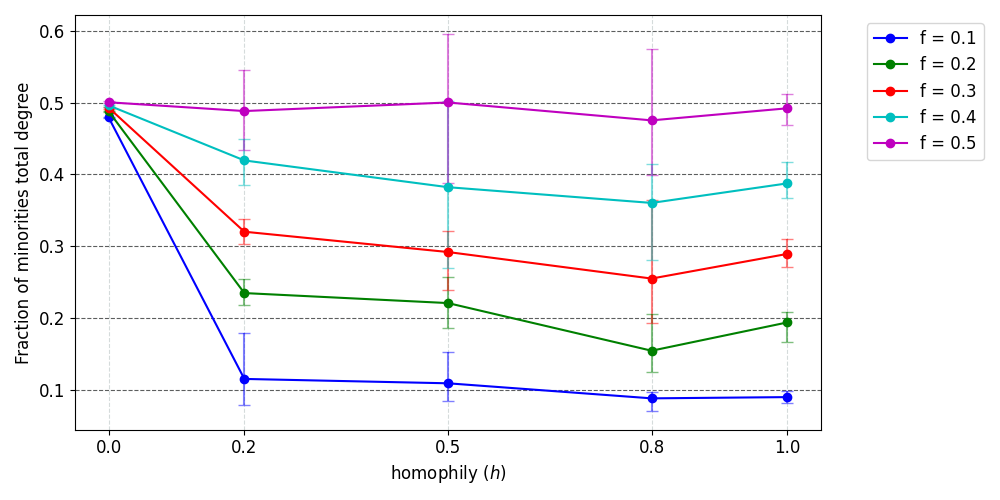
\includegraphics[trim=0 5 0 10, clip, width=0.75\textwidth]{images/mf_growth_tr.png}
	\caption{The fraction of total degree held by minority nodes for growing networks with \textbf{Twitter-Rank}.}
	\label{mf_growth_tr_fig}
\end{SCfigure}

\begin{figure}[h!]
	\centering
	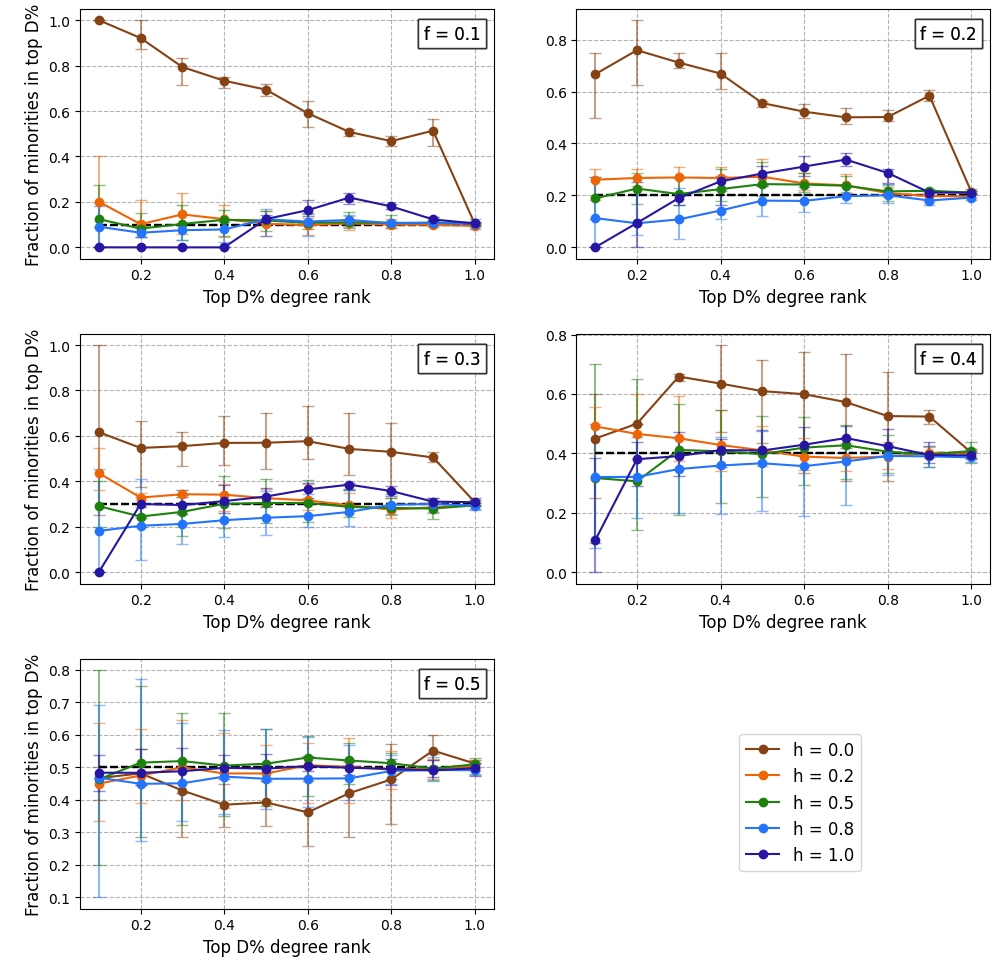
\includegraphics[trim=0 10 0 5, clip, width=1.0\textwidth]{images/top_growth_tr.png}
	\caption{The fraction of minority nodes found in top D\% nodes ranked according to degree in growing networks with \textbf{Twitter-Rank}. A black dotted line at each plot shows the actual fraction of minority nodes in the network.}
	\label{top_growth_tr_fig}
\end{figure}

First we would be discussing about behavior in the \textbf{heterophilic} regime. At $h=0$, majorities are recommended an incredibly high amount of majority nodes and minorities are recommended minority nodes (this increases with the group size). For a smaller minority group size at $h=0$, it can be seen that there is more majorities which are recommended for minorities but with time this also drops. This explains why at $h=0$, the nodes do not attain very high degrees as can be seen in the degree distribution plot (figure \ref{dd_growth_tr_fig}). The degree growth is quite high for minorities because over time they still receive a healthy number of majority node connections. The majorities however do not receive that much of minority connections so their degree growth is weak. 

At $h=0.2$, the distribution completely changes. At this phase majorities start getting recommended highly for both type of nodes. This provides the unbiased networks which have the fraction of total degrees close to that of the original group size (as seen in figure \ref{mf_growth_tr_fig}). We can see that although at the extreme case the minorities are overrepresented, as the homophily increases the network reaches a equal visibility relative to the group size. 

In the \textbf{homophilic} regime, at $h=0.8$ there is high number of majority node recommendations for both the majority and the minority nodes. Thus even in this case the degree is closer to the group size of the individual nodes. If we look at the fraction of total degrees held by minorities plot (figure \ref{mf_growth_tr_fig}) we see that minorities seem to be holding slightly lesser fraction of degree than its group size. This can be understood by the fact that while there is high number of recommendations of majorities for both groups, the count of majorities recommended for majorities is slightly less in the homophilic regime. At the complete homophily case since most of the network is possibly disconnected, nodes start getting recommendations from its own group as we had also observed previously in the \textit{PA-Homophily} case. 

An observation which we can make specifically from the degree growth plot (\ref{dg_growth_tr_fig}) is that in the range of $h=[0.2, 0.8]$ the degree growth is quite dampened. We believe that since in this method the user's `circle of trust' is formed based on the personalized PageRank mechanism the recommendation of nodes have a local effect, as in the recommended nodes belong in the locality of the seeker nodes. Thus, the degree of specific nodes might not grow as fast as seen in other methods. This also signifies that we do not reach very high degrees for nodes in this method as can be seen from the degree distribution plot (figure \ref{dd_growth_tr_fig}) compared to let's say \textit{Adamic-Adar} which causes the network nodes to have really high degrees. 

\subsection{Experimental Results : Ranked-Bandit}

In our experiments we modified the value of ranking factor ($r$) with values $\{0.0, 0.5, 1.0\}$ to influence the effect of ranking in the recommendation list $L_{v_{i}}$ for node $v_{i} \in V_{i}$. We however observed that this ranking factor $r$ provides very little difference to our plots. If we check the count of the recommendations which nodes get for different ranking values (check additional plots in appendices), we can see that at higher $r$ values there is a slight difference in the homophilic region for the number of nodes which are recommended for each type. This is however very minimal and we do not believe that it influences the choice of network nodes connection. In this section we display only the plots for the $r$ value of 1.0. The plots for other $r$ values can be found in the additional plots in appendices. 

\begin{figure}[h!]
	\centering
	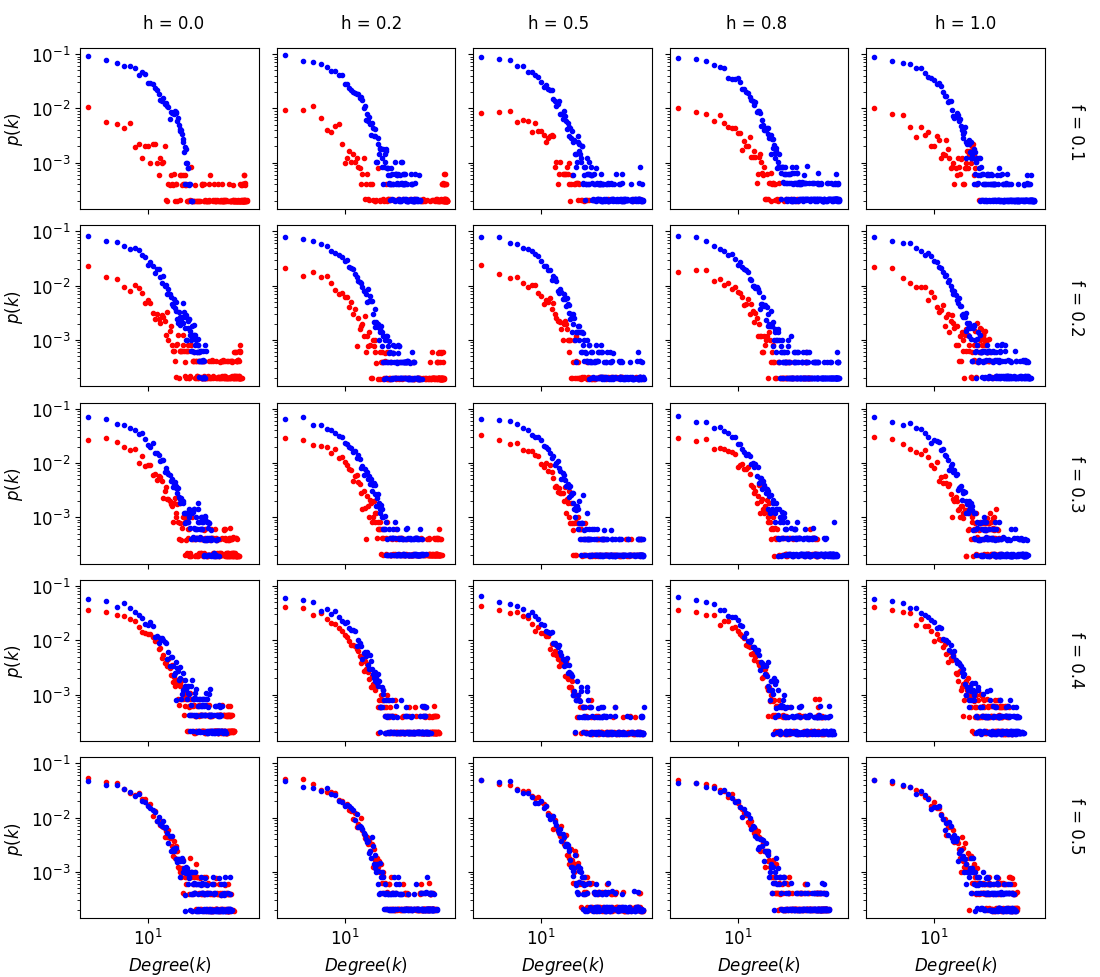
\includegraphics[width=1.0\textwidth]{images/dd_growth_rb10.png}
	\caption{Degree distribution for growing networks with \textbf{Ranked-Bandit ($r = 1.0$)}.The minority fractions are provided at the right-side of each row and the homophily values are specified at the top of each column. Degree distribution for the majority and minority nodes are visualized using blue and red plot points respectively.}
	\label{dd_growth_rb10_fig}
\end{figure}

\begin{figure}[h!]
	\centering
	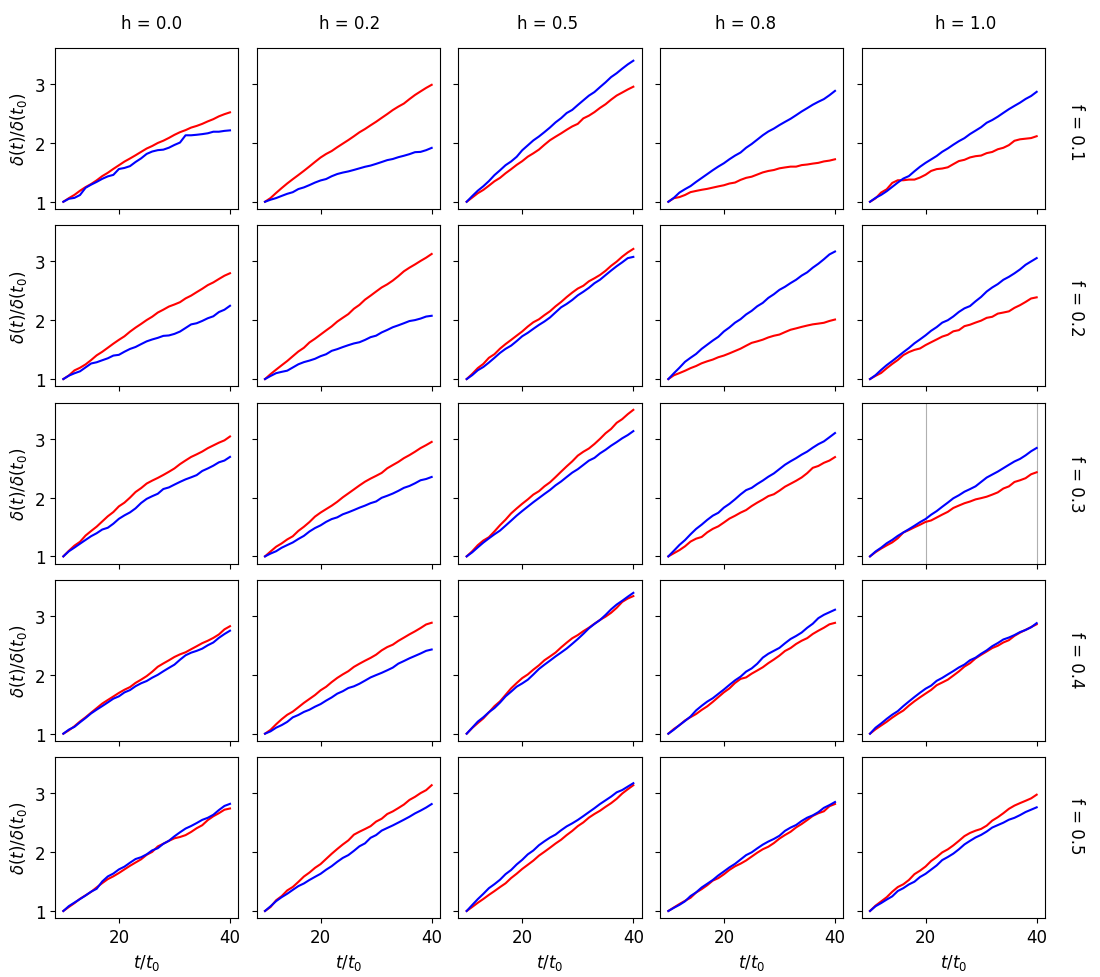
\includegraphics[width=1.0\textwidth]{images/dg_growth_rb10.png}
	\caption{Degree growth for growing networks with \textbf{Ranked-Bandit ($r = 1.0$)}. The minority fractions are provided at the right-side of each row and the homophily values are specified at the top of each column. Degree growth for minority and majority node is visualized using red and blue color plot lines respectively.}
	\label{dg_growth_rb10_fig}
\end{figure}

\begin{SCfigure}[1][h!]
	\centering
	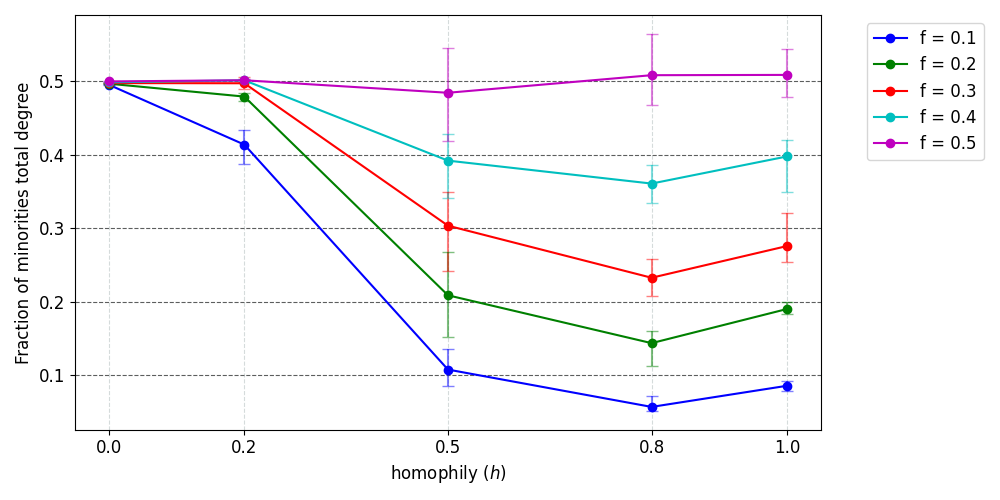
\includegraphics[trim=0 5 0 10, clip, width=0.75\textwidth]{images/mf_growth_rb10.png}
	\caption{The fraction of total degree held by minority nodes for growing networks with \textbf{Ranked-Bandit ($r = 1.0$)}.}
	\label{mf_growth_rb10_fig}
\end{SCfigure}

\begin{figure}[h!]
	\centering
	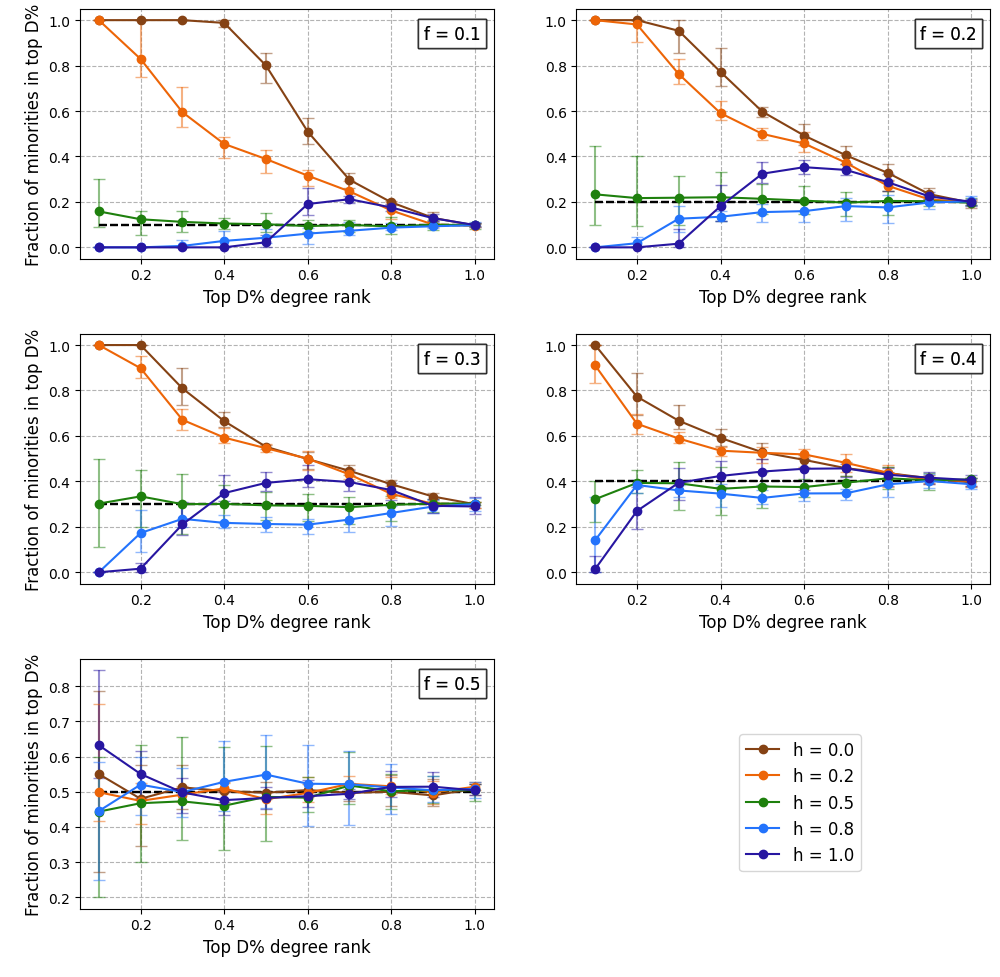
\includegraphics[trim=0 10 0 5, clip, width=1.0\textwidth]{images/top_growth_rb10.png}
	\caption{The fraction of minority nodes found in top D\% nodes ranked according to degree in growing networks with \textbf{Ranked-Bandit ($r = 1.0$)}. A black dotted line at each plot shows the actual fraction of minority nodes in the network.}
	\label{top_growth_rb10_fig}
\end{figure}

If we observe the degree distribution while using the \textbf{Ranked-Bandit} method in figure \ref{dd_growth_rb10_fig}, we can see that owing to the use of the click model (which in turn uses the Karimi model \cite{karimi2018homophily}) we see the patterns which could be observed in figure \ref{dd_growth_pa_fig} also observed here. In the heterophilic regime, minority nodes hold higher degrees than majority nodes and as we move towards the homophilic regime, this reverses. Also as we move down the figure towards increasing minority group sizes we can see that the degree distribution for both group of nodes can be perceived as similar. This is an indication that the reinforcement learning model could correctly learn the connection tendencies and thus push our system towards formation of a network which is similar to what we might observe with the Karimi model.

The degree growth plot given in figure \ref{dg_growth_rb10_fig} is also quite similar to the degree growth plot in figure \ref{dg_growth_pa_fig}. In the case of $h=0$, we see higher degree growth than expected for majority nodes, which might be possible because of the randomness ($\mu$) factor and also the fact that majorities are chosen more for connections in algorithmic growth.

The fraction of degree held by minorities plot (figure \ref{mf_growth_rb10_fig}) has similarities in all cases with figure \ref{mf_growth_pa_fig} other than at $h=0.2$. Comparing with the plot for \textit{PA-Homophily} we can see that at $h=0.2$ the minority nodes seem to be holding a higher fraction of the total degree than what is observed for \textit{PA-Homophily} for all minority group sizes ($f$). This would signify that minorities are much more over-represented in the heterophilic regime in \textbf{Ranked-Bandit} method.

We see a over-representation of minority nodes in heterophilic regime and under-representation in the homophilic regime when looking at the Top D\% degree ranked nodes in figure \ref{top_growth_rb10_fig}. Also as we observed before in figure \ref{mf_growth_rb10_fig}, we see that at $h=0.2$, minorities are much more over-represented in comparison to what we had observed before in the case of \textit{PA-Homophily}. This means that in the heterophilic regime, the bias for minorities is much higher in this kind of a recommendation system. 

\subsection{Experimental Results : Top-Rank}

Similar to \textbf{Ranked-Bandit}, we modified the value of ranking factor ($r$) with values $\{0.0, 0.5, 1.0\}$ to influence the effect of ranking in the recommendation list $L_{v_{i}}$ for node $v_{i} \in V_{i}$. We observe slight differences in the number of minority and majority nodes which form the recommendation list, but our belief is that this does not affect the final structure of the model. Here we show the results for $r=1.0$, and the plots for the other $r$ values can be found in the appendices.

Looking at the degree distribution plots (figure \ref{dd_growth_top10_fig}), we observe similarities with \textbf{Ranked-Bandit}. In the heterophilic regime, we can see that minority nodes clearly hold higher degrees at lower minority-group sizes. As the group-size increases, majorities tend to hold as much of higher degrees as minorities, a phenomenon observed before too. As we move towards the homophilic regime, the majority nodes hold higher degrees than the minority nodes owing to the preference of same-group attachments and higher volume of majority nodes. This effect is neutralized out as we move down towards equal group-sizes. 

\begin{figure}[h!]
	\centering
	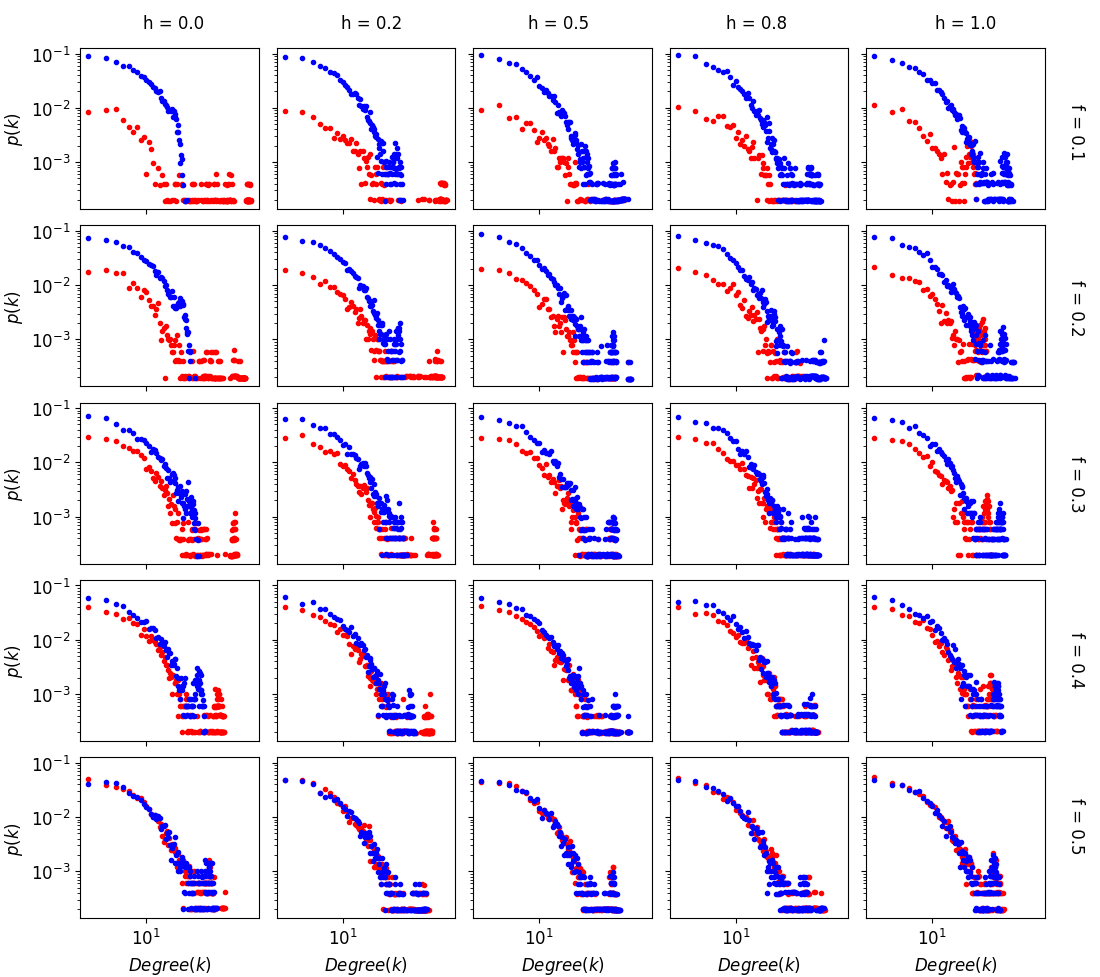
\includegraphics[width=1.0\textwidth]{images/dd_growth_top10.png}
	\caption{Degree distribution for growing networks with \textbf{Top-Rank ($r = 1.0$)}. The minority fractions are provided at the right-side of each row and the homophily values are specified at the top of each column. Degree distribution for the majority and minority nodes are visualized using blue and red plot points respectively.}
	\label{dd_growth_top10_fig}
\end{figure}

Upon looking at the degree growth plot (figure \ref{dg_growth_top10_fig}), we see that in the heterophilic regime the degree growth is much higher for minority nodes than majority nodes. This phenomenon has also been previously observed for synthetic networks which were influenced by the Karimi growth model. As we move towards the homophilic regime, the majority nodes gain higher degrees over minorities. We see a much faster degree growth for minorities than majority nodes in the heterophilic regime, and this can be attributed to the fact that the \textbf{Top-Rank} method is able to recommend minority nodes to majority with a much higher confidence (by having them at a greater precedence level). This confidence at placing nodes at higher precedence slots could also be the reason why at $f=0.1$ and $h=1$ we see that the minority nodes have higher degree growth than majority nodes.

\begin{figure}[h!]
	\centering
	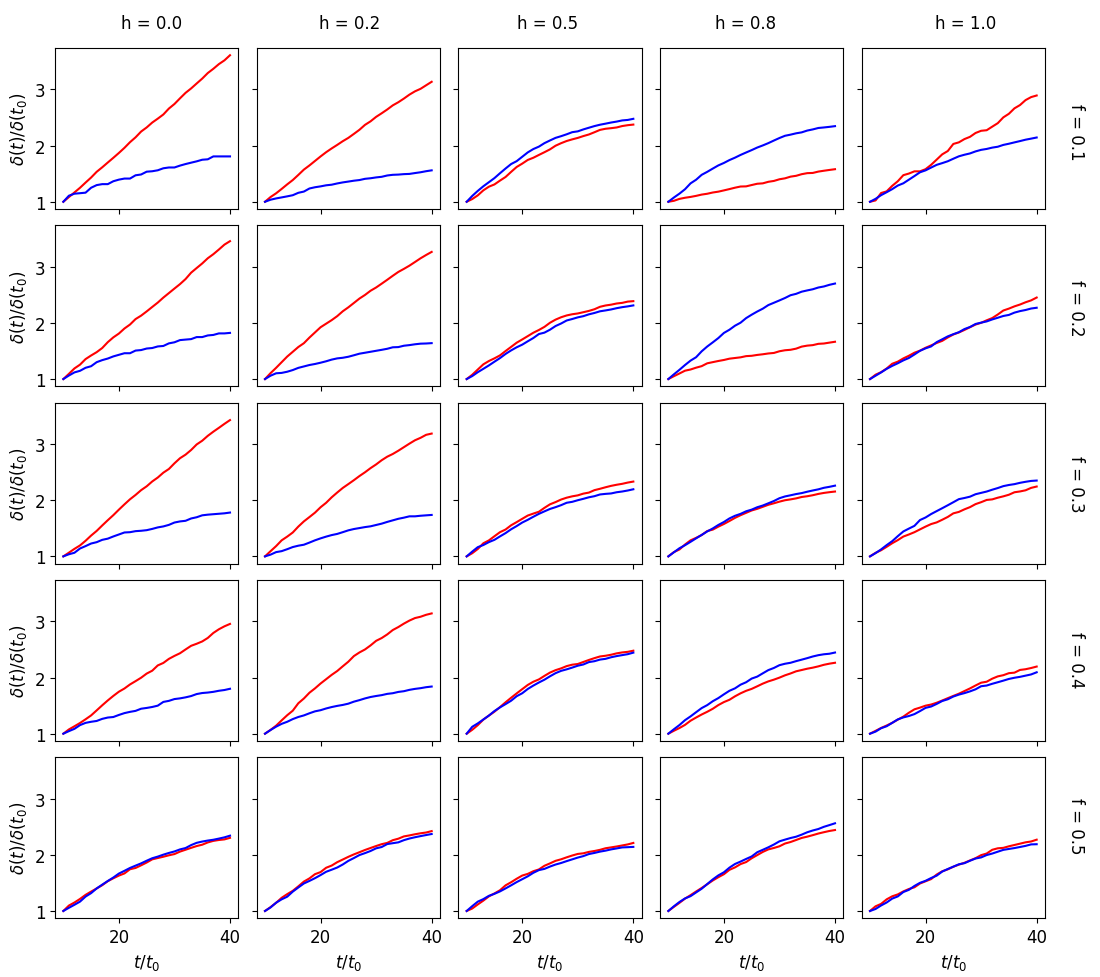
\includegraphics[width=1.0\textwidth]{images/dg_growth_top10.png}
	\caption{Degree growth for growing networks with \textbf{Top-Rank ($r = 1.0$)}. The minority fractions are provided at the right-side of each row and the homophily values are specified at the top of each column. Degree growth for minority and majority node is visualized using red and blue color plot lines respectively.}
	\label{dg_growth_top10_fig}
\end{figure}

Looking at the total degree held by minority nodes (figure \ref{mf_growth_top10_fig}) we also see similar results to what is expected. In the heterophilic regime, minority nodes hold higher degrees than their group-size, while in the homophilic regime they hold lower degrees which eventually is balanced out at complete homophily.

\begin{SCfigure}[1][h!]
	\centering
	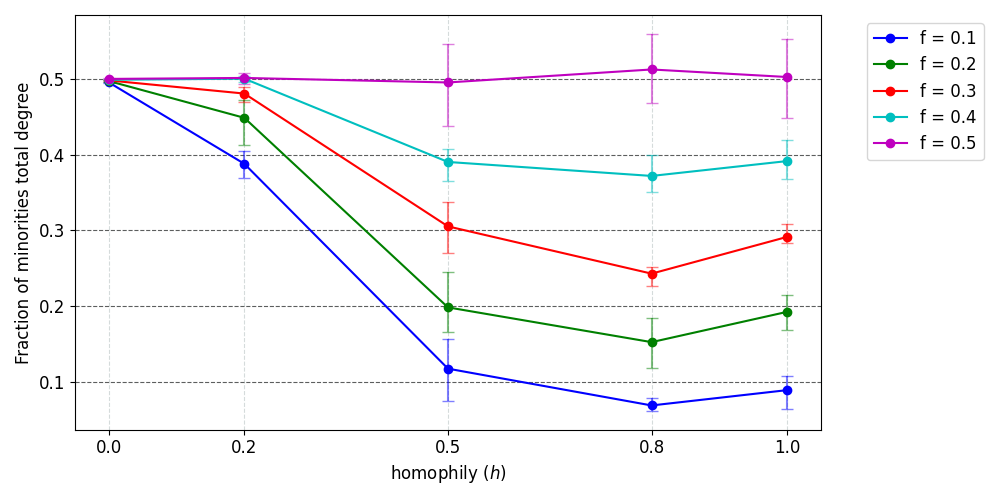
\includegraphics[trim=0 5 0 10, clip, width=0.75\textwidth]{images/mf_growth_top10.png}
	\caption{The fraction of total degree held by minority nodes for growing networks with \textbf{Top-Rank ($r = 1.0$)}.}
	\label{mf_growth_top10_fig}
\end{SCfigure}

The fraction of minorities in top D\% graph (figure \ref{top_growth_top10_fig}) show minorities being over-represented in the heterophilic regime, and underrepresented in the homophilic regime. This factor is also reduced as the minority group size increases. This shows the bias which is present in the click model is assimilated by the \textbf{Top-Rank} model as well, which causes the network to form in a similar fashion as the karimi model. 

\begin{figure}[h!]
	\centering
	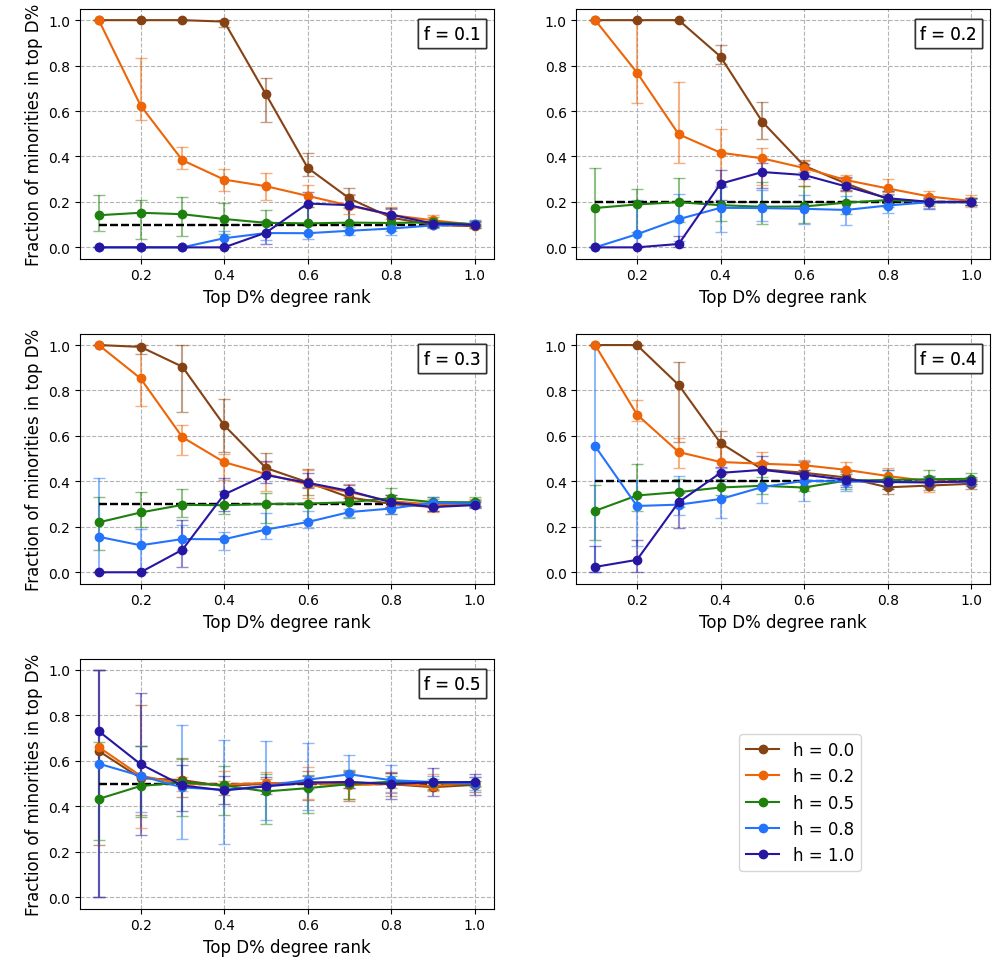
\includegraphics[trim=0 10 0 5, clip, width=1.0\textwidth]{images/top_growth_top10.png}
	\caption{The fraction of minority nodes found in top D\% nodes ranked according to degree in growing networks with \textbf{Top-Rank ($r = 1.0$)}. A black dotted line at each plot shows the actual fraction of minority nodes in the network.}
	\label{top_growth_top10_fig}
\end{figure}

\subsection{Summarized Findings}

We list down our major observations from the experiments on Growing Networks below.

\begin{enumerate}
	\item In \textbf{PA-Homophily} and the \textbf{reinforcement methods} we see similar plot patterns as observed for pre-generated static networks. This is due to the use of a \textit{click model} which is similar to the synthetic network generation method. It also shows that our reinforcement learning methods were able to correctly imbibe the traits of network and can be tuned internally to give better unbiased recommendations.
	
	\item The Randomness factor ($\mu$) in algorithm \ref{growing_network_model} causes the minorities to have over-representation in the complete homophily regime as there are connections established between nodes from opposite groups even in the case of complete homophily.
	
	\item \textbf{Adamic-Adar} is able to produce networks which are unbiased. This is possible at all cases of homophily other than in the strict heterophily case. Use of this recommendation method could lead to the evolution of a naturally balanced network with correct visibility for groups. Also it is observed that nodes tend to obtain really high degrees in this scenario.
	
	\item \textbf{Twitter-Rank} also provides us with correct representation of groups according to their groups sizes. The degree growth for networks using this recommendation mode is very slow owing to the use of personalized PageRank mechanism to form user's `circle of trust'. This makes node recommendations localized in nature.
\end{enumerate}
% Chapter 5
\chapter{Case Study}
\label{case_study}
\thispagestyle{empty}

In this chapter we focus on our research goal \textbf{RG1.2} as defined in section \ref{research_goals}. In the previous chapter we had worked with synthetic networks and after having conducted several experiments with them with various parameters we wish to now analyze the bias in recommendations for some empirical networks. We start the chapter by talking about the empirical data we wish to use in our thesis and how we process it and set it up for our experiment. We also list down names and few of the network properties for each of the datasets which we use. In the next section we look at the results of our experiment on each of these datasets individually. We primarily analyze the disparate visibility bias for each of the chosen datasets.

\section{Setup}

We work on the \textbf{Facebook100} \cite{traud2012social} dataset published by Traud et. al. in 2011. This huge dataset contains snapshots of Facebook \textit{`friendship networks'} for 100 universities across the United States of America. We choose 4 datasets among the 100 for our thesis and use our recommendation methods on them to receive the recommended nodes list on which we carry out the disparate visibility analysis as we had done previously for \textit{static networks} in section \ref{static_networks}.

\subsection{Dataset overview}

Table \ref{table_facebook_datadet} gives an overview of the networks we choose from the \textbf{Facebook100} dataset to carry out our experiments. The \textbf{NetworkID} is the same as used to identify individual networks in the original dataset. We choose \textit{gender} as the node attribute to distinguish nodes belonging to the \textit{minority} or \textit{majority} group. The \textbf{Minority} column in the table shows the gender representing the minority group in each network. The fraction of nodes which belong to the minority group is given as $f$. We estimate the homophily value for each group using the method outlined by Karimi et. al. \cite{karimi2018homophily}. The minority and majority homophily values are given as $h_{minority}$ and $h_{majority}$ respectively. As we had mentioned earlier in \ref{back_networks}, real-world networks exhibit asymmetric homophily, which we can observe here for the chosen empirical networks. All values for $f$, $h_{minority}$ and $h_{majority}$ have been rounded off to 2 decimal places for our experiments.

\begin{table}[h]
	\centering
	\begin{tabular}{ |c|c|c|c|c|c|c| }
		\hline
		\textbf{Network ID} & \textbf{Total nodes} & \textbf{Total edges} & \textbf{Minority} & \textbf{$f$} & \textbf{$h_{minority}$} & \textbf{$h_{majority}$} \\
		\hline
		Caltech36 & 703 & 15464 & female & 0.32 & 0.75 & 0.6 \\
		Reed98 & 865 & 15948 & male & 0.42 & 0.73 & 0.7 \\
		%Haverford76 & 1350 & 53904 & male & 0.46 & 0.73 & 0.82 \\
		Simmons81 & 1422 & 30486 & male & 0.01 & 0.47 & 0.87 \\
		Swarthmore42 & 1521 & 53726 & male & 0.49 & 0.72 & 0.78 \\
		\hline
	\end{tabular}
	\caption{Details of chosen empirical networks from \textbf{Facebook100} dataset}
	\label{table_facebook_datadet}
\end{table}

We parse the original dataset, which is provided as a sparse matrix to form our own network adjacency matrices. For each network multiple nodes are found to not possess the \textit{gender} information. We choose to discard such nodes and the edges they form from our final network. 

\subsection{Experimental Setup}

For each of the networks $G(V,E)$ chosen by us (as listed in table \ref{table_facebook_datadet}) we use the \textit{Topological} and \textit{Reinforcement} recommender methods (as detailed in chapter \ref{recommender_methods}) to get a recommendation list $L_{v}$ for each node $v \in V$.

Once we have received this recommendation list, we measure the Disparate visibility \cite{fabbri2020effect} for the recommendations (similar to what we did in section \ref{static_networks}). 

\section{Results}

\subsection{Caltech36}

For the network \textbf{Caltech36} \textit{females} form the minority group with 32\% of the nodes belonging to this group. The minority group has a homophily value of 0.75 which is slightly higher than the majority group homophily value of 0.6. 

\begin{SCfigure}[1][h!]
	\centering
	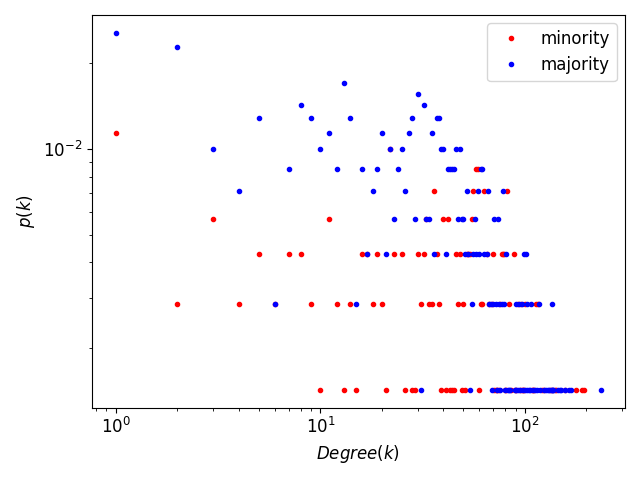
\includegraphics[trim=0 10 0 10, clip, width=0.75\textwidth]{images/dd_caltech.png}
	\caption{Degree distribution for \textbf{Caltech36}}
	\label{dd_caltech}
\end{SCfigure}

Looking at the degree distribution plot (figure \ref{dd_caltech}) we can see that both majority and minority nodes hold quite high degrees. Since both the groups are homophilic in nature with minority being more homophilic, this kind of distribution can be expected for the minority fraction of 0.3. 

\begin{SCfigure}[1][h!]
	\centering
	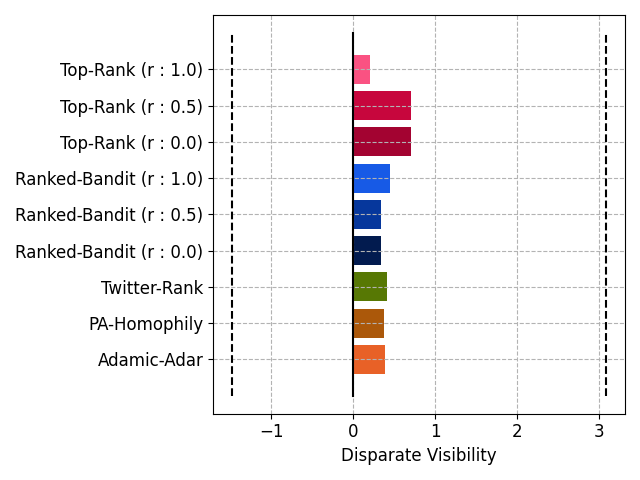
\includegraphics[trim=0 10 0 10, clip, width=0.75\textwidth]{images/dv_caltech.png}
	\caption{Disparate Visibility for \textbf{Caltech36}. Black dotted lines represent the range for the disparate visibility measure given the minority fraction and the solid black line shows the equal visibility mark at 0.}
	\label{dv_caltech}
\end{SCfigure}

Upon using our recommender methods, we find that the disparate visibility (figure \ref{dv_caltech}) is positive, which means that the minority nodes are more visible in recommendations than majorities. This result holds for all recommender methods used. The range of disparate visibility measure for this network lies between [-1.48, 3.08]. 

In our earlier experiments with measuring disparate visibility for static networks in section \ref{static_dv} we had assumed that for a homophilic regime the networks would have higher visibility for majorities. However, here we see that at the homophilic regime minorities are more visible. We however did not have information for the disparate visibility measure at homophily values of $h=0.6$ or $h=0.7$. Thus we might have missed information in our experiments which we can observe in this case. 

For the \textbf{PA-Homophily} method we can deduce that minorities are more visible owing to only slightly high homophily value for majorities and a greater homophily among minorities. This would mean that for both type of nodes there is a higher chance of having minorities as node recommendations. This is also seen in the \textbf{reinforcement methods}. In the case of \textbf{Top-Rank} we see much more visibility for minorities at $r=0.0$ and $r=0.5$, but this visibility decreases from others in the case of $r=1.0$. Here we see that the ranking factor actually has a much more sever effect than what we had observed previously in our experiments with static networks. What we can deduce is that since both minority and majority nodes have higher degrees and they both have only slightly varying homophily, the ranking factor in this case plays a major role in boosting the probability for nodes in \textit{click model}. Lesser visibility for minorities would however mean that the Top-Rank method has a higher mix of majority and minority nodes at upper precedence partitions. This is what causes the minority visibility to drop.

\subsection{Reed98}

For the network \textbf{Reed98}, \textit{males} form the minority group with 42\% of the nodes belonging to this group. The minority group has a homophily value of 0.73 which is very close to the majority group homophily value of 0.7, thus having almost symmetric homophily in this network. 

\begin{SCfigure}[1][h!]
	\centering
	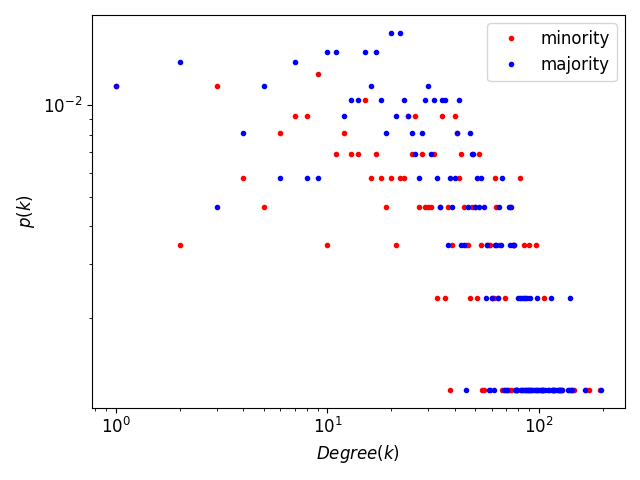
\includegraphics[trim=0 10 0 10, clip, width=0.75\textwidth]{images/dd_reed.png}
	\caption{Degree distribution for \textbf{Reed98}}
	\label{dd_reed}
\end{SCfigure}

Looking at the degree distribution plot (figure \ref{dd_reed}) we can see that both the majority and minority nodes hold high degrees. Since the network is moderately homophilic, with the minority group size quite high this can be expected with both groups supporting themselves. 

\begin{SCfigure}[1][h!]
	\centering
	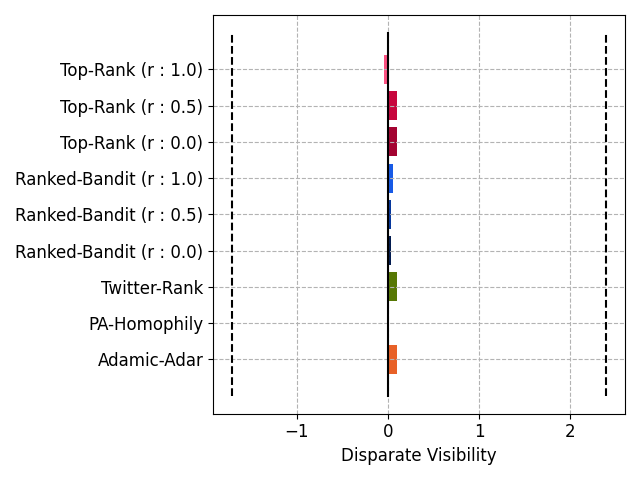
\includegraphics[trim=0 10 0 10, clip, width=0.75\textwidth]{images/dv_reed.png}
	\caption{Disparate Visibility for \textbf{Reed98}. Black dotted lines represent the range for the disparate visibility measure given the minority fraction and the solid black line shows the equal visibility mark at 0.}
	\label{dv_reed}
\end{SCfigure}

From the disparate visibility plot (figure \ref{dv_reed}), upon using our recommender methods on the network, we find that visibility for both groups borders the equal visibility mark. 

We had seen almost equal visibility for a minority size of $f=0.4$ in our synthetic network experiments too. The results corroborate with our findings for this network.

The range for disparate visibility measure for this network lies between [-1.72, 2.4]. Most values are slightly positive which shows that the minority group is at a very slight advantage, but this is very negligible ($\leq 5\%$). The \textbf{Top-Rank} method at $r=1.0$ however shows opposite behavior than the rest, putting majorities as more visible. The behavior which we had seen earlier in the case of \textbf{Caltech36} is thus seen here too for Top-Rank(r=1.0).

\subsection{Simmons81}

For the network \textbf{Simmons81}, \textit{males} form the minority group with only 1\% of the nodes belonging to this group. The minority group has a homophily value of 0.47 while the majority group has a homophily value of 0.87. This is a group with a very less minority who connects in an almost group-agnostic way while the majority has strong homophilic tendencies. So while the majority nodes have strong in-group support they also get connections from the minorities.

\begin{SCfigure}[1][h!]
	\centering
	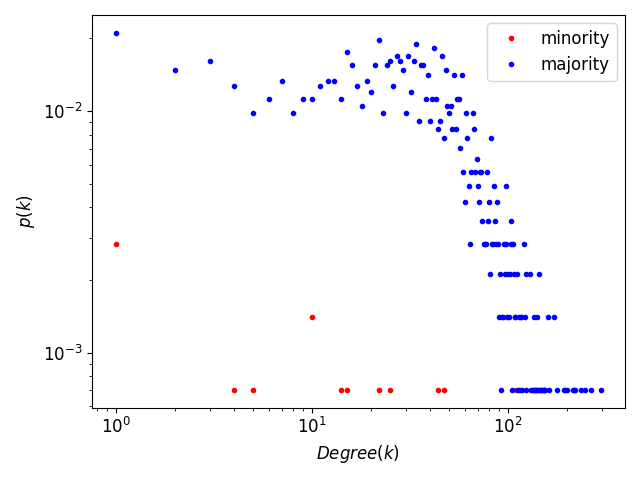
\includegraphics[trim=0 10 0 10, clip, width=0.75\textwidth]{images/dd_simmons.png}
	\caption{Degree distribution for \textbf{Simmons81}}
	\label{dd_simmons}
\end{SCfigure}

Looking at the degree distribution plot (figure \ref{dd_simmons}) we see that the majority nodes hold much higher degrees compared to the minority as we could expect looking at the homophily values. While a fair amount of majority nodes have degrees above 100, the maximum degree a minority node holds is far less than 100. This shows that majority nodes are much more well-connected than minorities.

\begin{SCfigure}[1][h!]
	\centering
	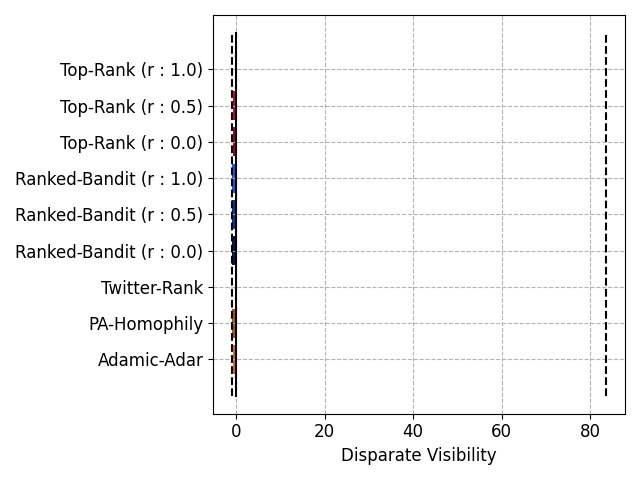
\includegraphics[trim=0 10 0 10, clip, width=0.75\textwidth]{images/dv_simmons.png}
	\caption{Disparate Visibility for \textbf{Simmons81}. Black dotted lines represent the range for the disparate visibility measure given the minority fraction and the solid black line shows the equal visibility mark at 0.}
	\label{dv_simmons}
\end{SCfigure}

From the disparate visibility plot (figure \ref{dv_simmons}), upon using our recommender methods on the nodes in the network, we find that visibility is higher for majority nodes. The range of disparate visibility measure for this network lies in the range of [-1.01, 83.65].

Since the majorities have high homophily and the minorities have almost neutral homophily, the majorities would be winning in the recommendations game in the \textbf{PA-Homophily} and subsequently the \textbf{reinforcement methods} cases. For both the majority and minority nodes there would be more majority nodes which would be suggested. Also since the minorities are so few in number most of them would already be connected with other minorities thus further increasing chances of majorities to be recommended. If the minority group size was higher we would probably see a higher minority visibility for our network. 

\subsection{Swarthmore42}

For the network \textbf{Swarthmore42}, \textit{males} barely form the minority group with 49\% of the nodes belonging to this group. The minority group has a homophily value of 0.72 while the majority group has a homophily value of 0.78. This is a network with equal node-group sizes exhibiting almost symmetric homophilic behavior.

\begin{SCfigure}[1][h!]
	\centering
	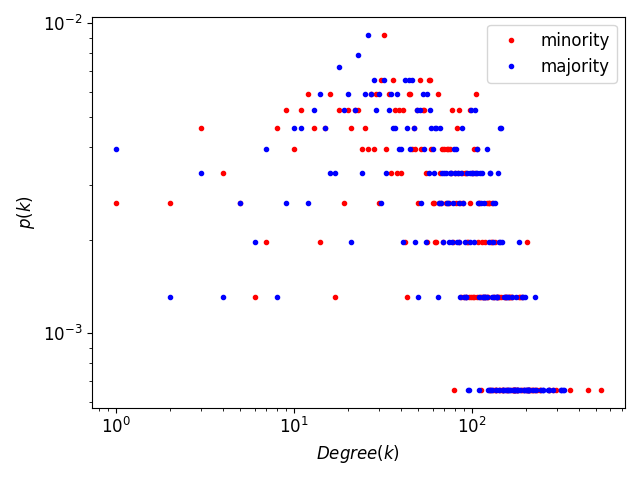
\includegraphics[trim=0 10 0 10, clip, width=0.75\textwidth]{images/dd_swarthmore.png}
	\caption{Degree distribution for \textbf{Swarthmore42}}
	\label{dd_swarthmore}
\end{SCfigure}

Looking at the degree distribution plot (figure \ref{dd_swarthmore}) we see that both majority and minority nodes have an almost equal distribution. The plot however does not strictly demonstrate the properties of a scale-free network as in there are lower degree nodes with lower probability also present in the network. The number of edges in this network is also quite high which would mean that there the nodes are well connected with a higher average degree.

\begin{SCfigure}[1][h!]
	\centering
	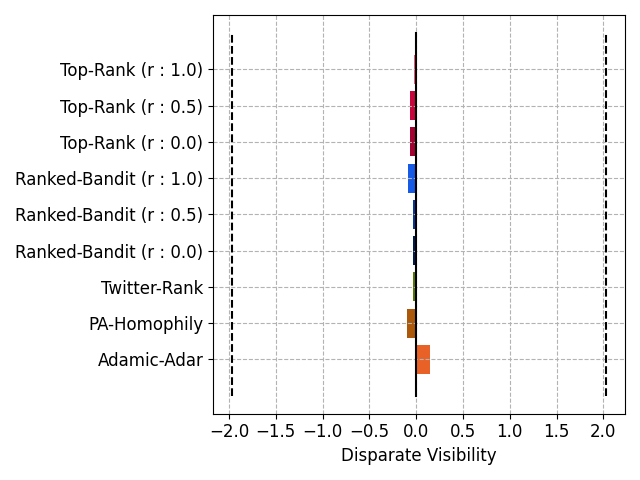
\includegraphics[trim=0 10 0 10, clip, width=0.75\textwidth]{images/dv_swarthmore.png}
	\caption{Disparate Visibility for \textbf{Swarthmore42}. Black dotted lines represent the range for the disparate visibility measure given the minority fraction and the solid black line shows the equal visibility mark at 0.}
	\label{dv_swarthmore}
\end{SCfigure}

From the disparate visibility plot (figure \ref{dv_swarthmore}), upon using our recommender methods on the network, we find that visibility for most cases is only negligibly higher for majority nodes. This suggests that the recommendations are quite balanced for both groups as we could have expected for a equal group size. The range of disparate visibility measure for this network lies between [-1.97, 2.03]. 

For the case of \textbf{Adamic-Adar} we see that the minority seems to have higher visibility than what is projected by the other methods. As we know that the Adamic-Adar method is completely structure dependent this could mean the network structure favors minorities in certain way. However this difference is very negligible to make a concrete comment on why this happens.

\section{Summary}

Using the various recommendation methods $R$ as we had defined in chapter \ref{recommender_methods} we carry out our experiment on empirical networks to get recommendations for each node in the networks. We use selected network from the \textbf{Facebook100} dataset to measure the disparate visibility found in the recommendations.

From our experiments we only see the \textbf{Caltech36} network give a higher visibility score in favor of minorities. The other networks either have an almost equal group-size or have a very small minority size which puts them close to the equal visibility measure.

In \textbf{Caltech36} we see that minorities are more visible which is different from what we were expecting from our experiments on synthetic networks. This clearly points to a limitation of our work since we do not know the disparate visibility behavior in the in-between homophily cases. Our consideration of homophily values for experiments is limited and the behavior in more such cases is something worth exploring in the future.
% Chapter 6
\chapter{Discussions}
\label{discussions}
\thispagestyle{empty}

In this chapter we discuss the limitations of our work and also look into future directions in which our work could be extended. 

\section{Limitations}

We look at the different limitations our work faces by moving through each individual section of our thesis.

\subsubsection{Methods}
We list down below some limitations in our approach for the methods chosen by us.

\begin{enumerate}
	\item For the method \textbf{Twitter-Rank} based on \textit{Who-To-Follow} architecture of Twitter, we do not consider some of the steps outlined in the original approach. In the method outline by Gupta et. al. \cite{gupta2013wtf}, they talk about using multiple iterations of the SALSA method for computing final scores while we use only a single iteration due to limited computation power. Also, in their work they hint about using homophily in the network as a parameter to further enhance user-recommendations but they do not detail any steps on how they wish to use it. Our consideration of the method is completely unconcerned of the homophily parameter, and using that would definitely give us very different results as compared to what we see in our experiments. 
	
	\item We construct a \textbf{click model} in section \ref{click_model} based on the \textit{``Preferential Attachment with Homophily''} model by Karimi et. al. \cite{karimi2018homophily}. However, this model is very simplistic in nature and fails to capture the essence of clicks on recommendations provided in the real-world social networks. We use this model due to the lack of any real-world data on recommendations and user choices, thus making broad assumptions in the case of \textit{reinforcement methods}. A reinforcement model is only as good as its click model, hence this is a big limitation for our study.
\end{enumerate}

\subsubsection{Synthetic Networks}
The synthetic networks generated for our research goals have very few nodes. For both \textit{Static networks} and \textit{Growing networks} we use only 1000 node networks. Our choice of less number of nodes is due to computational constraints.

In the case of \textit{static networks}, we needed to compute recommendations for 1000 nodes by each recommendation method, where each method takes a considerable amount of time. In the case of \textit{growing networks} we grew our networks for 10000 iterations, which gives us roughly 1000 nodes (with an organic growth probability of 0.1). Roughly 9000 of those iterations require recommendations which has a high computational cost associated with it. Having less number of nodes in our simulated network along with having fewer simulations for each case gives us somewhat unstable results as can be seen in the error bars for different plots.

\subsubsection{Case Study}
For the networks we choose from \textbf{Facebook100} we are forced to choose networks having less number of nodes to use less computation time for recommendations. Although there were networks which could give us varied homophily and minority fractions, we were unable to look at the recommendation bias for them.

Another major limitation is also the use of our \textit{click model} from section \ref{click_model}. This click model is in not representative of the way Facebook network users form connections and is only a theoretical generalization. The ideal scenario would be to have clicking behavior data for Facebook users recommendation and using them to train our reinforcement learning models to get more aligned predictions.

\section{Future Work}

There are a couple of directions which could be interesting to explore going forward from here.

\begin{enumerate}
	\item As we have mentioned in the limitations of our work, it would be good to conduct the experiments with larger synthetic networks. Also we use limited homophily values and hence many observations are missed. One such observation we already saw in our analysis of disparate visibility for empirical networks. Specially the nature of bias at homophily values range [0.2, 0.8] would be interesting to observe.
	
	\item We only consider undirected networks in our work, however in real-world there are many social networks which are directed (for example Twitter or Instagram). Analysis of these kinds of network would give broader understanding of bias in such networks.
	
	\item There are multiple other methods for node recommendation which we do not consider in our work. Exploring them could be interesting as our recommendation methods give slightly different results for disparate visibility than the methods which were used by Fabrri et. al. in \cite{fabbri2020effect}. Also, we consider only node attributes but some recommendation methods also consider edge attributes, like in the work of Backstorm et. al. \cite{backstrom2011supervised} which is possibly used for Facebook user recommendations. 
	
	\item We only use a single \textit{click model} for all our experiments. Most of the click model research is based around search query results and there is not much existing work for selection of users from recommended lists. This could be worthwhile to investigate if we wish to formulate reinforcement learning models for recommendation tasks. Thus collection of real-world data for clicking behavior in different online social networks would be imperative to such studies.
	
	\item Exploring ways to mitigate the bias in recommendations for the different methods is also something which could be studied. Our experiments do show huge bias specially in the heterophilic regime. How this bias can be handled so that the evolving networks would have balanced visibility is something worth exploring.
	
	\item For the empirical networks we only use \textit{gender} as the node attribute to differentiate nodes into groups. Using other attributes to create different groups and observing the homophily between them could also be another approach for studying these empirical networks.
\end{enumerate}
% Chapter 7
\chapter{Conclusion}
\label{conclusions}
\thispagestyle{empty}

Through our thesis we try to understand bias present in networks owing to the use of recommender systems which are an integral parts of any social network today. Constructing experiments through synthetic networks and also considering empirical networks for our study, we see the effect of 5 different recommender systems, among which two of the recommender systems we consider are novel to the user-recommendation scenario based on the \textit{reinforcement learning} methods. The \textit{reinforcement method} results closely follow that of the \textit{PA-Homophily} method since their underlying driving engine is similar which shows us that reinforcement learning models can be used in user recommendation scenarios too with proper training models. Our findings mostly show that there is greater bias in visibility in the heterophilic regime for minority nodes, and this bias is larger with a smaller minority group. Methods like \textit{Adamic-Adar} and \textit{Twitter-Rank} showed bias free network evolution and almost equal visibility for both groups across different homophily values. 

\subsubsection{Static synthetic Networks}
For the first part of our first research goal we look at static synthetic networks. These are synthetic networks which have been pre-generated using the \textit{Barabási-Albert with homophily network generation model} \cite{karimi2018homophily}. We tune parameters like homophily and the minority group size to get different networks. We then use our recommendation engines to get recommendations for all nodes in the networks. Upon receiving such recommendation lists we apply the disparate visibility measure to check if the nodes from different groups get visibility comparable to their group size. 

From our experiments we find that the minority visibility is much higher in the heterophilic regime for smaller minority group sizes. As the minority group size increases the visibility becomes equalized. In the homophilic regime, the relative visibility is found to be quite equal for both groups. We also find out that \textit{Adamic-Adar} and \textit{Twitter-Rank} methods produce recommendations for nodes having equal visibility.

\subsubsection{Growing synthetic Networks}
For the second research goal, we see how the network structure is evolved when they are grown over a certain number of iterations using the different recommendation systems. We vary different parameters like minority fraction and homophily values in these simulations and grow networks for 10000 iterations from scratch with the \textit{organic} and \textit{algorithmic} growth as is seen in real-world networks.

Our findings show that for both the \textit{PA-Homophily} and the \textit{reinforcement methods} the minorities are over-represented at the heterophilic regime and underrepresented in the homophilic regime. We find that \textit{Adamic-Adar} and \textit{Twitter-Rank} provides us with networks which have better visibility according to group size for all homophily values. In the case of \textit{Adamic-Adar} we see nodes in the network gaining very high degrees while in the case of \textit{Twitter-Rank} the nodes have a more distributed degree owing to the personalized PageRank approach used in its method.

\subsubsection{Empirical Networks}
For the second part of our first research goal we look at empirical networks. These are real-world static snapshots of networks. For our experiments we use 4 networks from the \textbf{Facebook100} \cite{traud2012social} dataset, which is a Facebook friendship network dataset for different universities in USA. 

We pre-process the networks to form adjacency matrices and use the gender attribute in the nodes to form the majority and minority groups. We estimate the homophily value in the network using the method outlined by Karimi et. al. \cite{karimi2018homophily}. We set up our experiment much like that for \textit{static synthetic networks}, where we use our recommendation systems to get recommendation lists for all nodes in the network and then look for the bias in recommendations using the disparate visibility measure.

In our results we find out a limitation for our study (while looking at the network \textbf{Caltech36}) which shows us that we lack data points of disparate visibility behavior for many networks which lie in different homophilies in-between which are not considered during our synthetic networks experiments.

Most of the networks we use in our study of empirical networks also have almost equal group sizes so they show near equal visibility. We observe that the \textit{Top-Rank} method at a ranking factor of $r=1.0$ (full ranking effect), shows a distinctly different behavior for all networks which is different than what we observe in our static network experiments.

\subsubsection{Future Work}
There are many limitations for our work like use of less number of nodes for synthetic networks, consideration of less variations of homophily and fewer simulations which can all be done for further better analysis of recommender bias in networks. Also collection and use of empirical data to understand clicking behavior of recommendations in social platforms would be a huge help in defining the click model for reinforcement methods. Working towards how to mitigate bias in the recommender systems for the generation of equal visibility networks in the growing mechanism is also another interesting extension to our work.

%%%%%%%%%%%%%%%%%%%%% Bibliography %%%%%%%%%%%%%%%%%%%%%% 
\addcontentsline{toc}{chapter}{Bibliography}
\printbibliography

% Appendix 
\begin{appendices}

\chapter{Analyzing Synthetic Data}
Here we provide additional visualizations which we generated for the purpose of our thesis for synthetic data analysis of \textit{growing networks} in section \ref{growing_networks}.

As we have detailed in algorithm \ref{growing_network_model}, we grow the synthetic networks for $t(=10000)$ iterations in our experiments for \textit{Growing Networks}. We visualize the change in count of minority and majority nodes in the recommendation list of length $k(=5)$ for recommendations to minority and majority nodes with progress in time. The iteration step-size considered for these plots is 1000.

Also for the \textit{reinforcement methods} we only provide the results for the ranking factor $r=1.0$ in the results section for \textit{growing networks}. Here we provide the additional plots for the ranking factor values of $r=\{0.0, 0.5\}$ for the \textit{Ranked-Bandit} and \textit{Top-Rank} recommender methods.

%\section{Experimental Results : PA-Homophily}

\begin{figure}[h!]
	\centering
	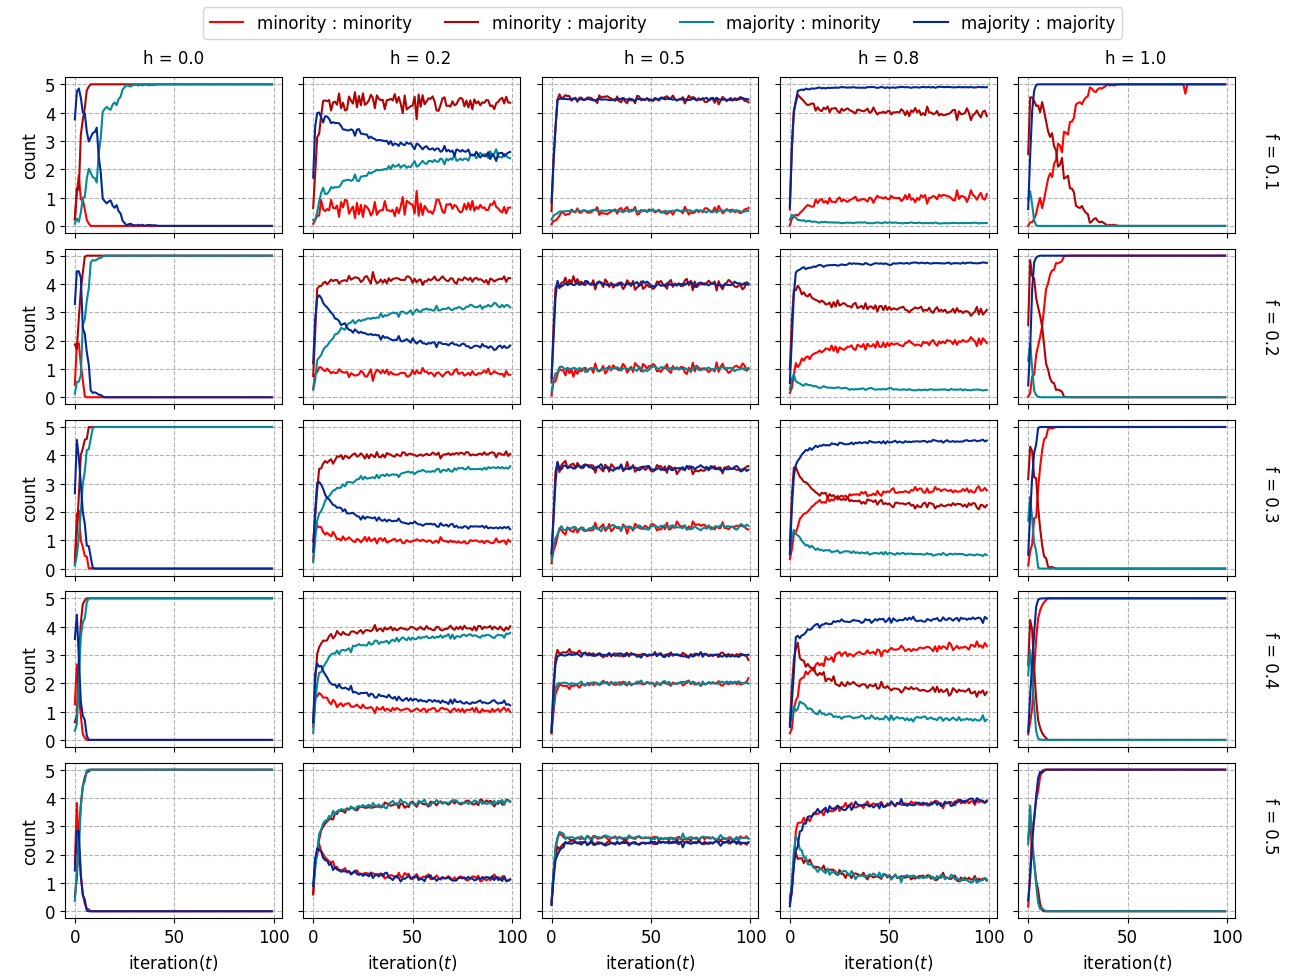
\includegraphics[width=1.0\textwidth]{images/count_pa.png}
	\caption{Count of nodes in the recommendation list over time for minority and majority nodes in a growing network aided with \textbf{PA-Homophily} recommender agent. Homophily values are specified above the respective columns and minority fractions are specified at the right side of the row. Light red plot line denotes count of minority nodes recommended for other minority nodes. Dark red plot line denotes count of majority nodes recommended for other minority nodes. Light blue line denotes count of minority nodes recommended for other majority nodes. Dark blue line denotes count of majority nodes recommended for other majority nodes.}
	\label{count_pa}
\end{figure}

%\section{Experimental Results : Adamic-Adar}

\begin{figure}[h!]
	\centering
	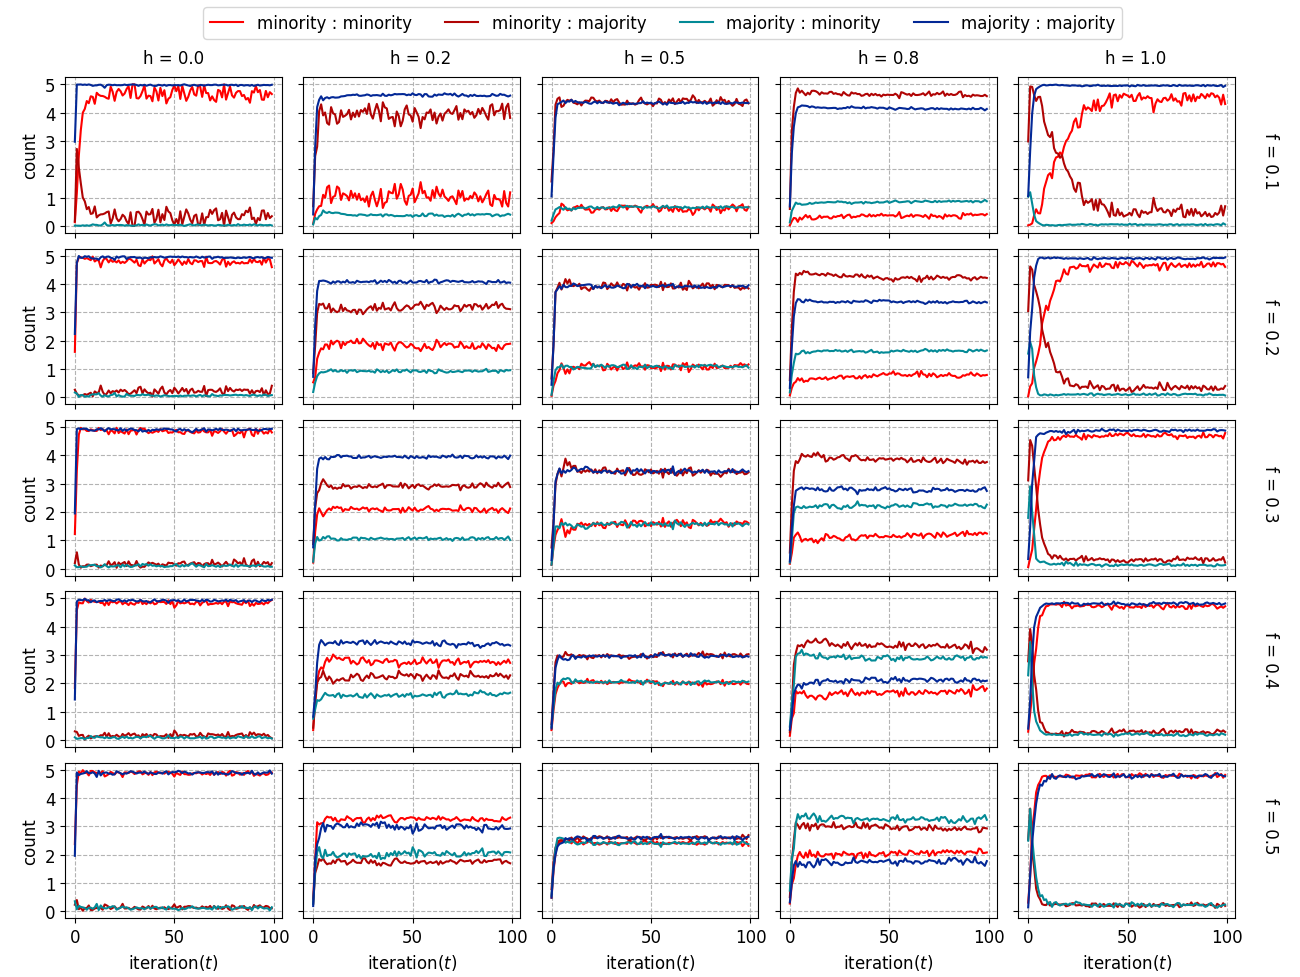
\includegraphics[width=1.0\textwidth]{images/count_aa.png}
	\caption{Count of nodes in the recommendation list over time for minority and majority nodes in a growing network aided with \textbf{Adamic-Adar} recommender agent. Homophily values are specified above the respective columns and minority fractions are specified at the right side of the row. Light red plot line denotes count of minority nodes recommended for other minority nodes. Dark red plot line denotes count of majority nodes recommended for other minority nodes. Light blue line denotes count of minority nodes recommended for other majority nodes. Dark blue line denotes count of majority nodes recommended for other majority nodes.}
	\label{count_aa}
\end{figure}

%\section{Experimental Results : Twitter-Rank}

\begin{figure}[h!]
	\centering
	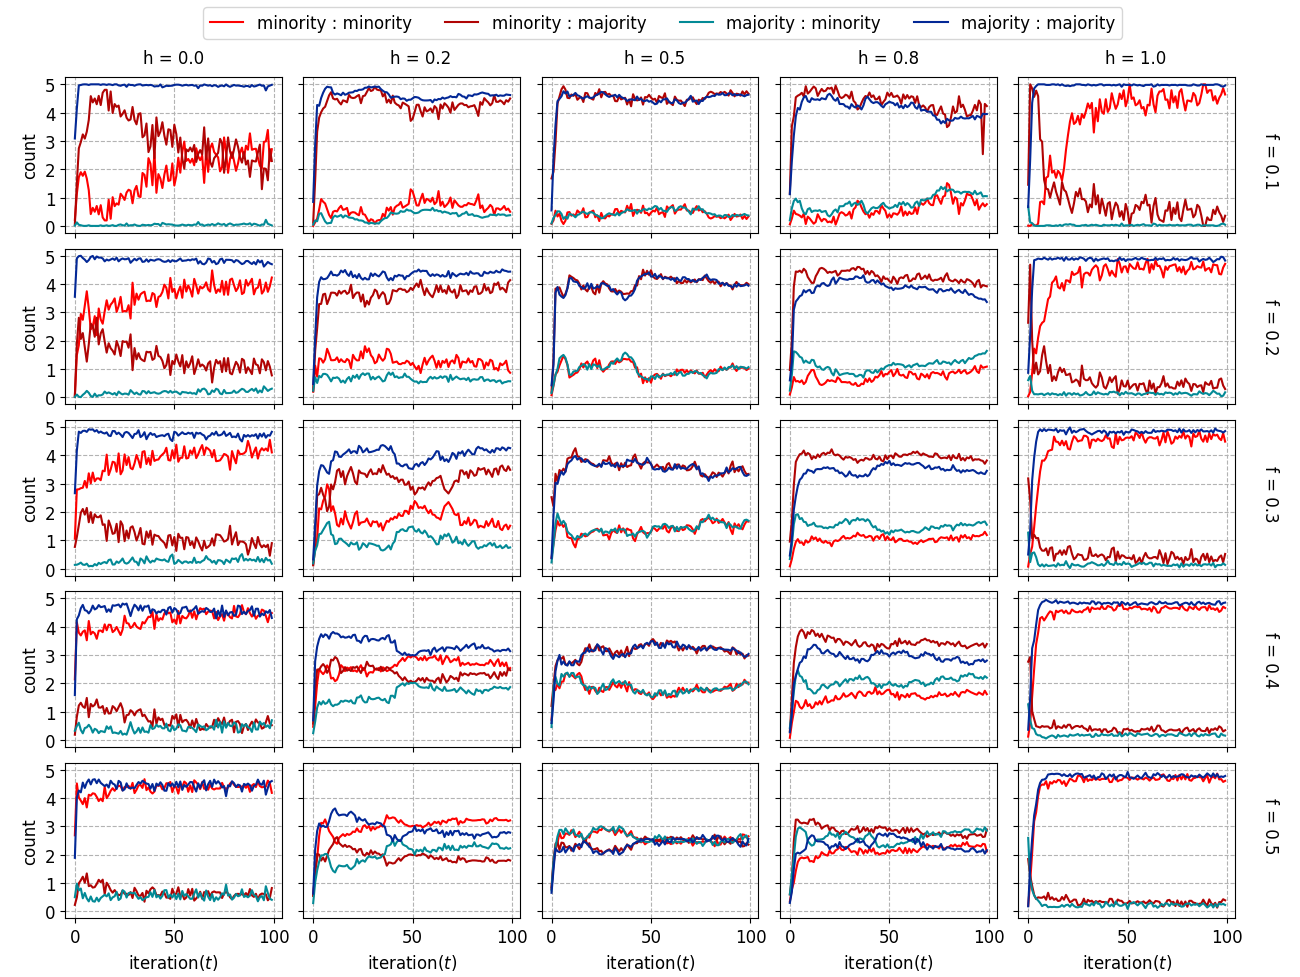
\includegraphics[width=1.0\textwidth]{images/count_tr.png}
	\caption{Count of nodes in the recommendation list over time for minority and majority nodes in a growing network aided with \textbf{Twitter-Rank} recommender agent. Homophily values are specified above the respective columns and minority fractions are specified at the right side of the row. Light red plot line denotes count of minority nodes recommended for other minority nodes. Dark red plot line denotes count of majority nodes recommended for other minority nodes. Light blue line denotes count of minority nodes recommended for other majority nodes. Dark blue line denotes count of majority nodes recommended for other majority nodes.}
	\label{count_tr}
\end{figure}

%\section{Experimental Results : Ranked-Bandit (r=0.0)}

\begin{figure}[h!]
	\centering
	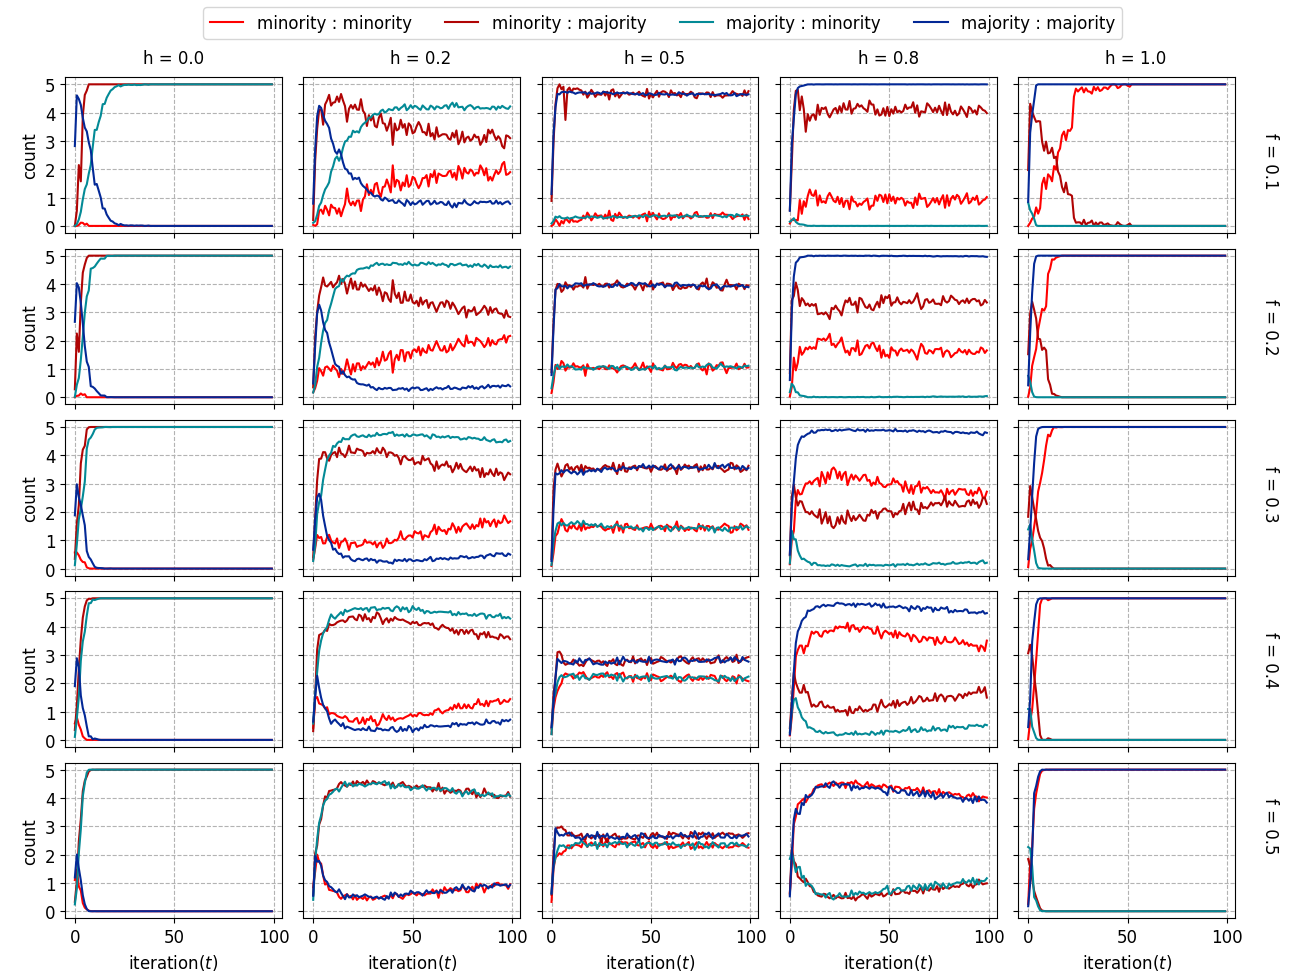
\includegraphics[width=1.0\textwidth]{images/count_rb00.png}
	\caption{Count of nodes in the recommendation list over time for minority and majority nodes in a growing network aided with \textbf{Ranked-Bandit}(r=0.0) recommender agent. Homophily values are specified above the respective columns and minority fractions are specified at the right side of the row. Light red plot line denotes count of minority nodes recommended for other minority nodes. Dark red plot line denotes count of majority nodes recommended for other minority nodes. Light blue line denotes count of minority nodes recommended for other majority nodes. Dark blue line denotes count of majority nodes recommended for other majority nodes.}
	\label{count_rb00}
\end{figure}

\begin{figure}[h!]
	\centering
	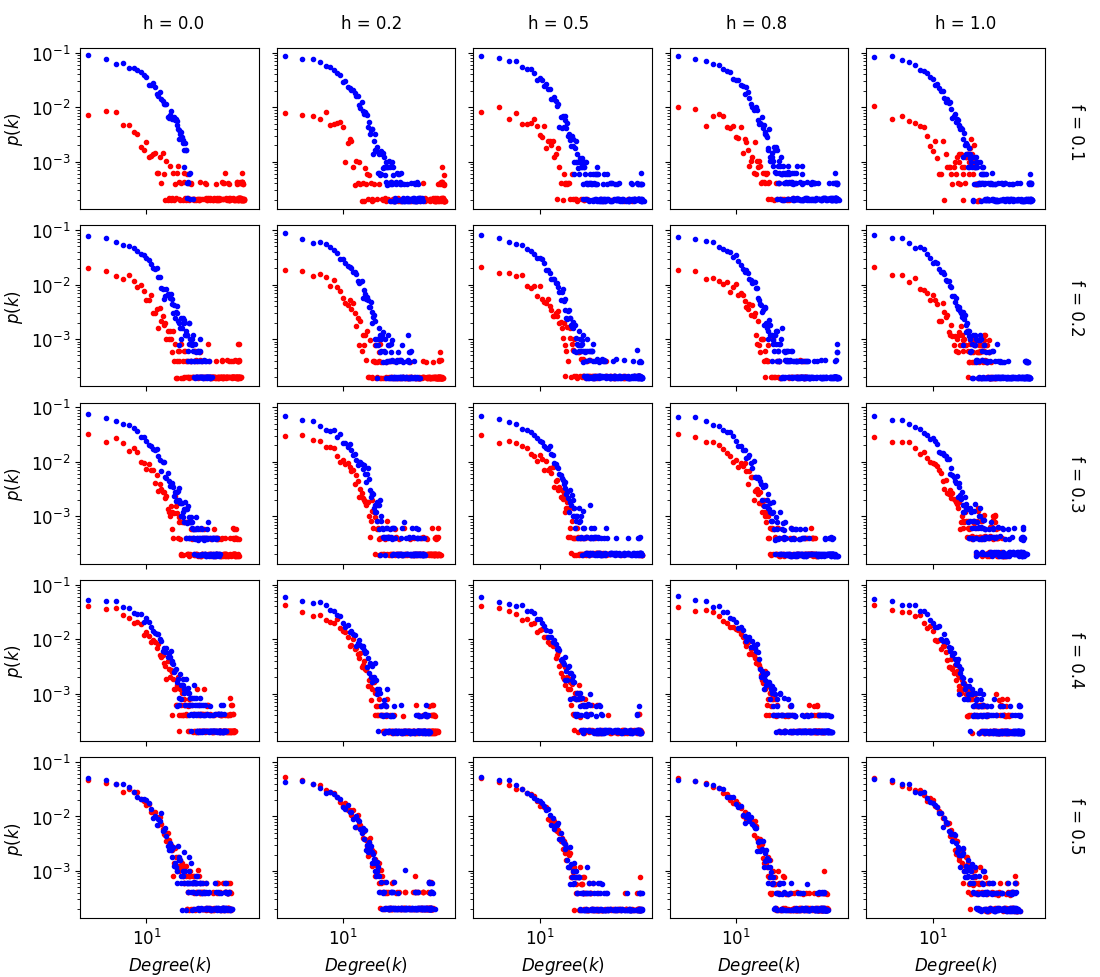
\includegraphics[width=1.0\textwidth]{images/dd_growth_rb00.png}
	\caption{Degree distribution for growing networks with \textbf{Ranked-Bandit ($r = 0.0$)}.The minority fractions are provided at the right-side of each row and the homophily values are specified at the top of each column. Degree distribution for the majority and minority nodes are visualized using blue and red plot points respectively.}
	\label{dd_growth_rb00_fig}
\end{figure}

\begin{figure}[h!]
	\centering
	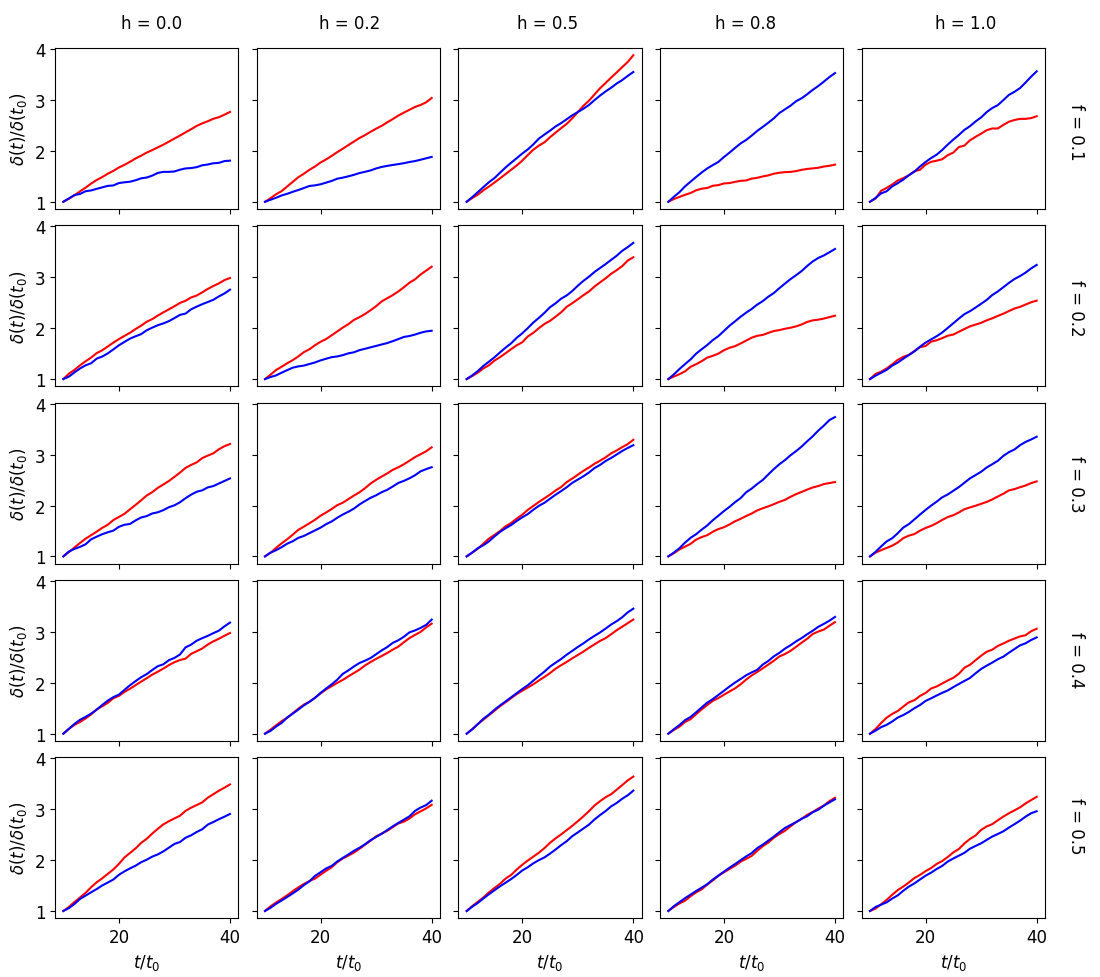
\includegraphics[width=1.0\textwidth]{images/dg_growth_rb00.png}
	\caption{Degree growth for growing networks with \textbf{Ranked-Bandit ($r = 0.0$)}. The minority fractions are provided at the right-side of each row and the homophily values are specified at the top of each column. Degree growth for minority and majority node is visualized using red and blue color plot lines respectively.}
	\label{dg_growth_rb00_fig}
\end{figure}

\begin{SCfigure}[1][h!]
	\centering
	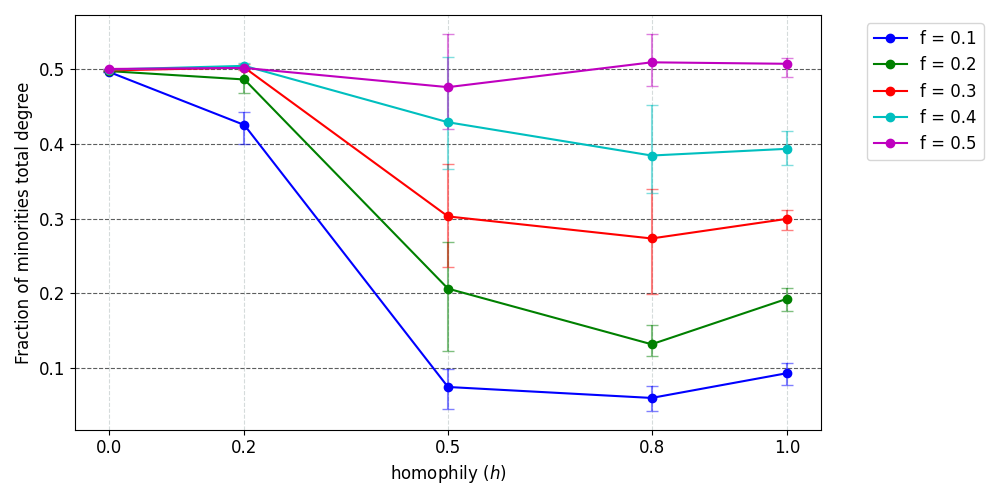
\includegraphics[trim=0 5 0 10, clip, width=0.75\textwidth]{images/mf_growth_rb00.png}
	\caption{The fraction of total degree held by minority nodes for growing networks with \textbf{Ranked-Bandit ($r = 0.0$)}.}
	\label{mf_growth_rb00_fig}
\end{SCfigure}

\begin{figure}[h!]
	\centering
	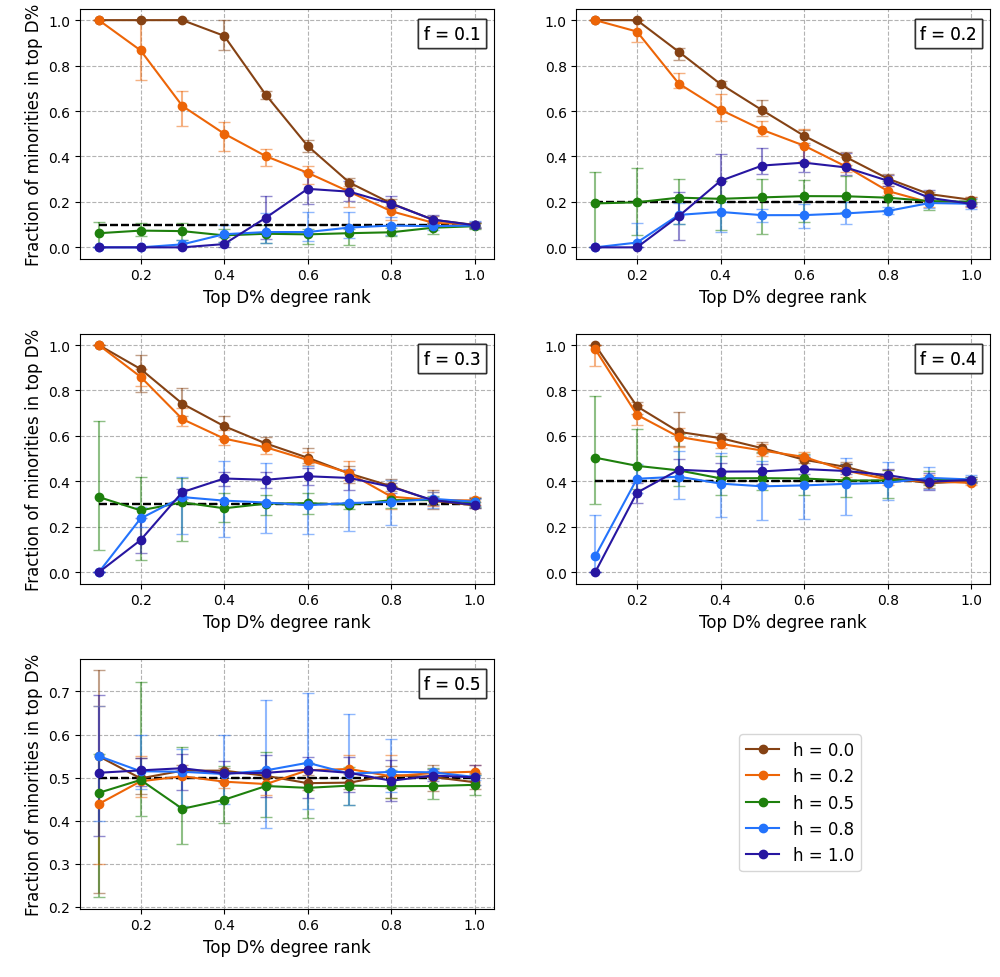
\includegraphics[trim=0 10 0 5, clip, width=1.0\textwidth]{images/top_growth_rb00.png}
	\caption{The fraction of minority nodes found in top D\% nodes ranked according to degree in growing networks with \textbf{Ranked-Bandit ($r = 0.0$)}. A black dotted line at each plot shows the actual fraction of minority nodes in the network.}
	\label{top_growth_rb00_fig}
\end{figure}

%\section{Experimental Results : Ranked-Bandit (r=0.5)}

\begin{figure}[h!]
	\centering
	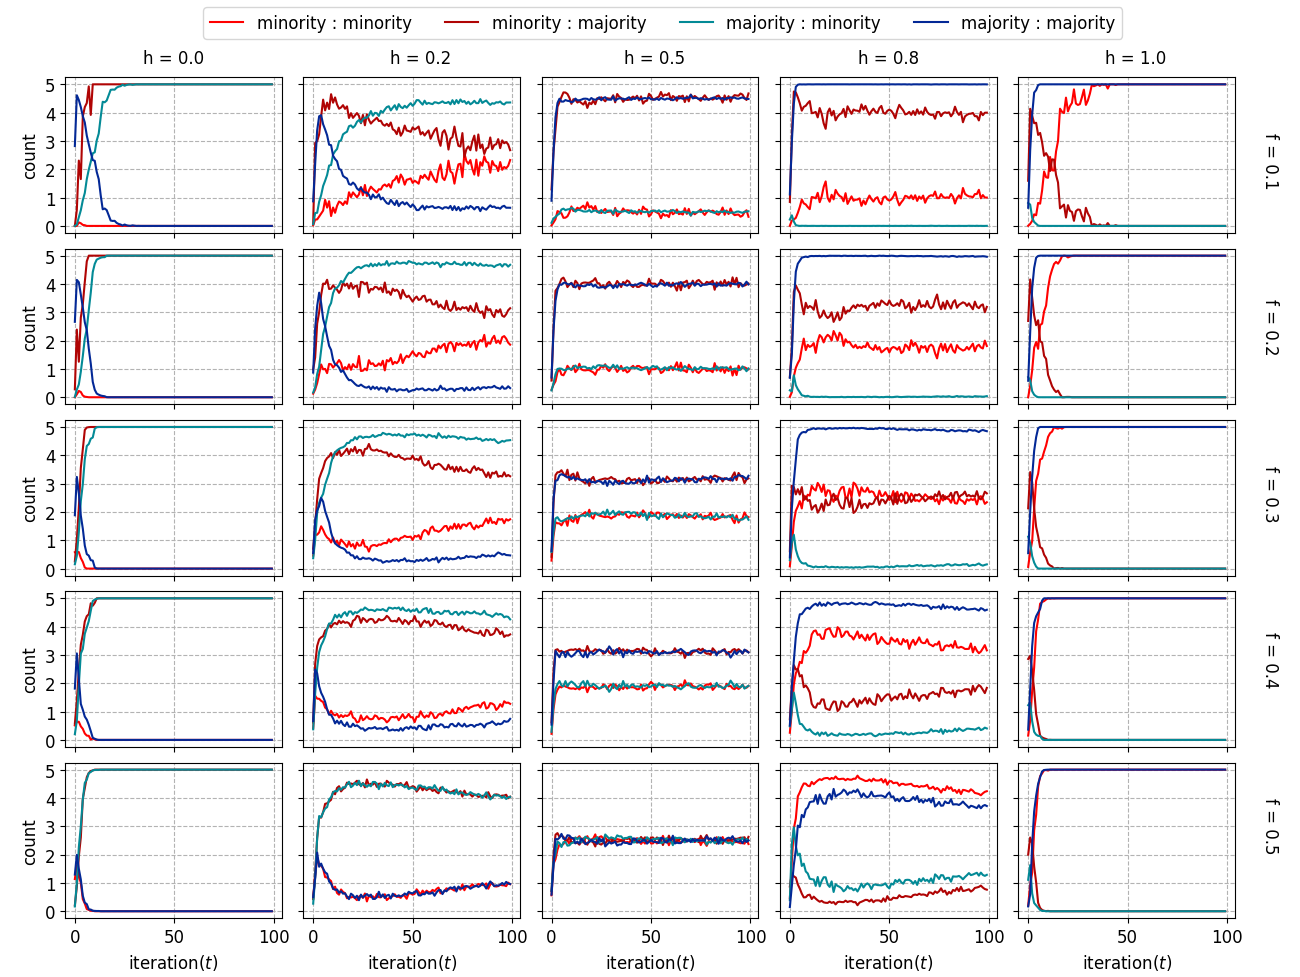
\includegraphics[width=1.0\textwidth]{images/count_rb05.png}
	\caption{Count of nodes in the recommendation list over time for minority and majority nodes in a growing network aided with \textbf{Ranked-Bandit}(r=0.5) recommender agent. Homophily values are specified above the respective columns and minority fractions are specified at the right side of the row. Light red plot line denotes count of minority nodes recommended for other minority nodes. Dark red plot line denotes count of majority nodes recommended for other minority nodes. Light blue line denotes count of minority nodes recommended for other majority nodes. Dark blue line denotes count of majority nodes recommended for other majority nodes.}
	\label{count_rb05}
\end{figure}

\begin{figure}[h!]
	\centering
	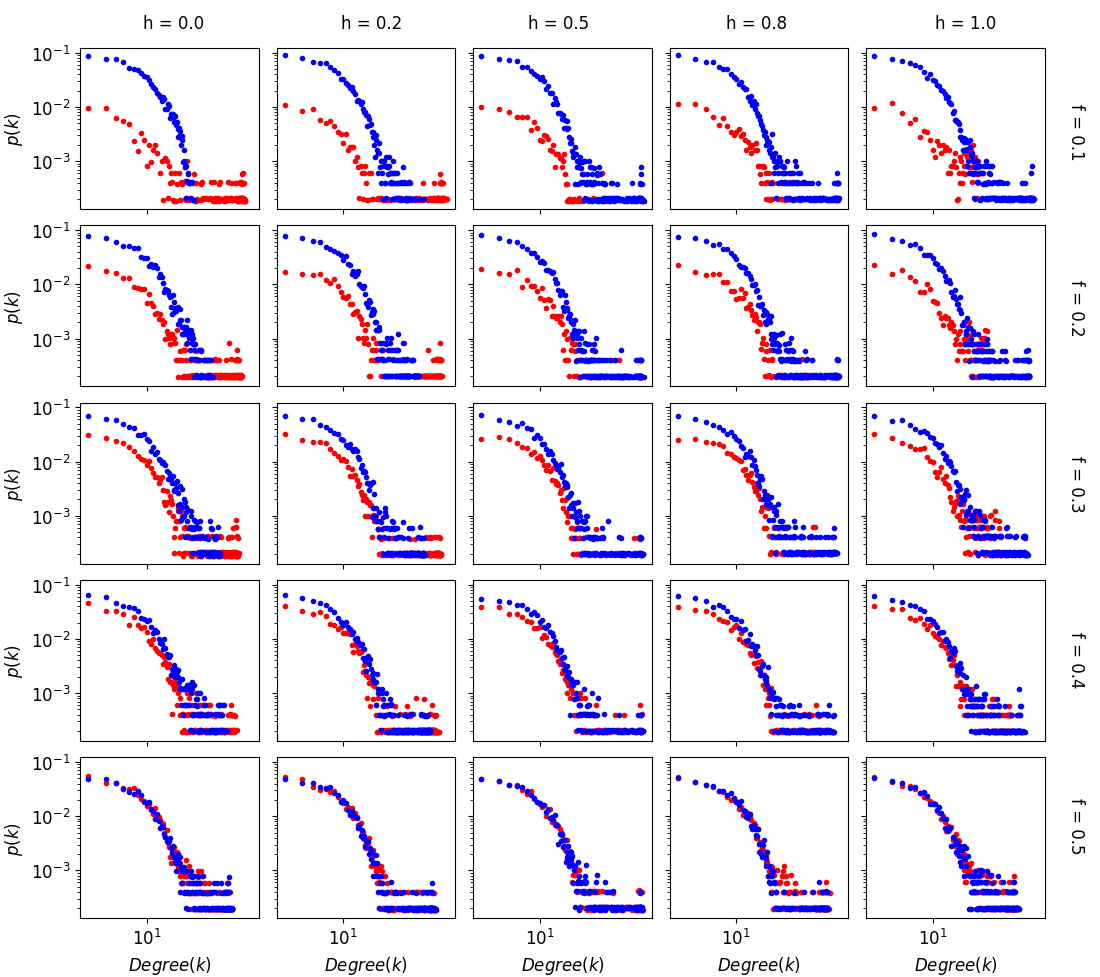
\includegraphics[width=1.0\textwidth]{images/dd_growth_rb05.png}
	\caption{Degree distribution for growing networks with \textbf{Ranked-Bandit ($r = 0.5$)}.The minority fractions are provided at the right-side of each row and the homophily values are specified at the top of each column. Degree distribution for the majority and minority nodes are visualized using blue and red plot points respectively.}
	\label{dd_growth_rb05_fig}
\end{figure}

\begin{figure}[h!]
	\centering
	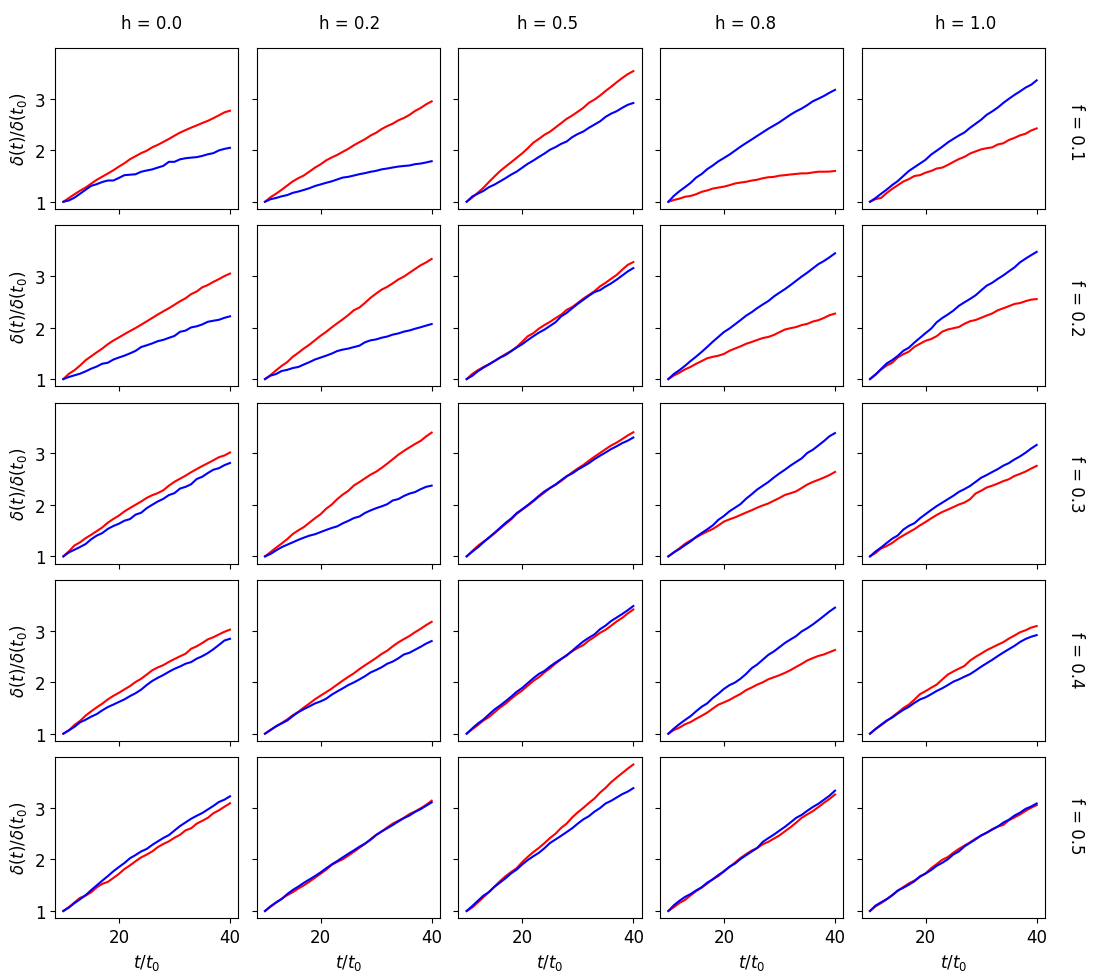
\includegraphics[width=1.0\textwidth]{images/dg_growth_rb05.png}
	\caption{Degree growth for growing networks with \textbf{Ranked-Bandit ($r = 0.5$)}. The minority fractions are provided at the right-side of each row and the homophily values are specified at the top of each column. Degree growth for minority and majority node is visualized using red and blue color plot lines respectively.}
	\label{dg_growth_rb05_fig}
\end{figure}

\begin{SCfigure}[1][h!]
	\centering
	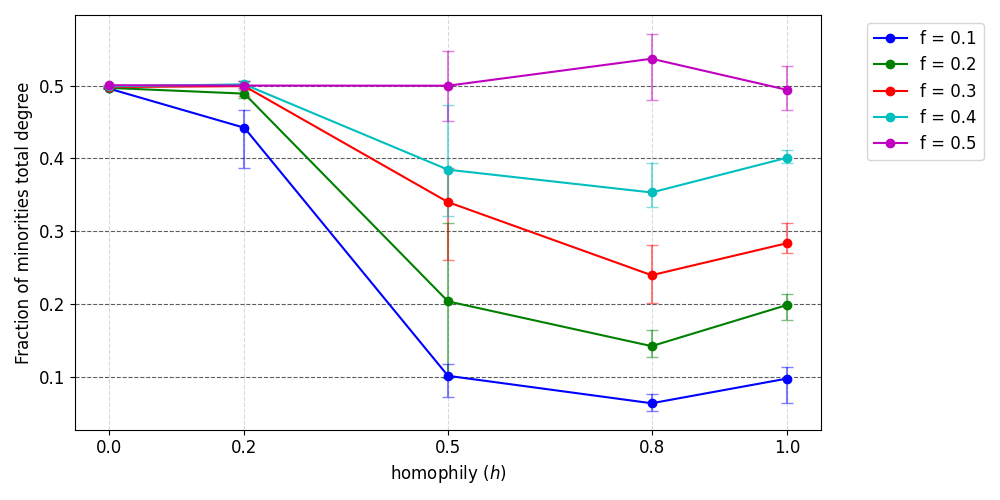
\includegraphics[trim=0 5 0 10, clip, width=0.75\textwidth]{images/mf_growth_rb05.png}
	\caption{The fraction of total degree held by minority nodes for growing networks with \textbf{Ranked-Bandit ($r = 0.5$)}.}
	\label{mf_growth_rb05_fig}
\end{SCfigure}

\begin{figure}[h!]
	\centering
	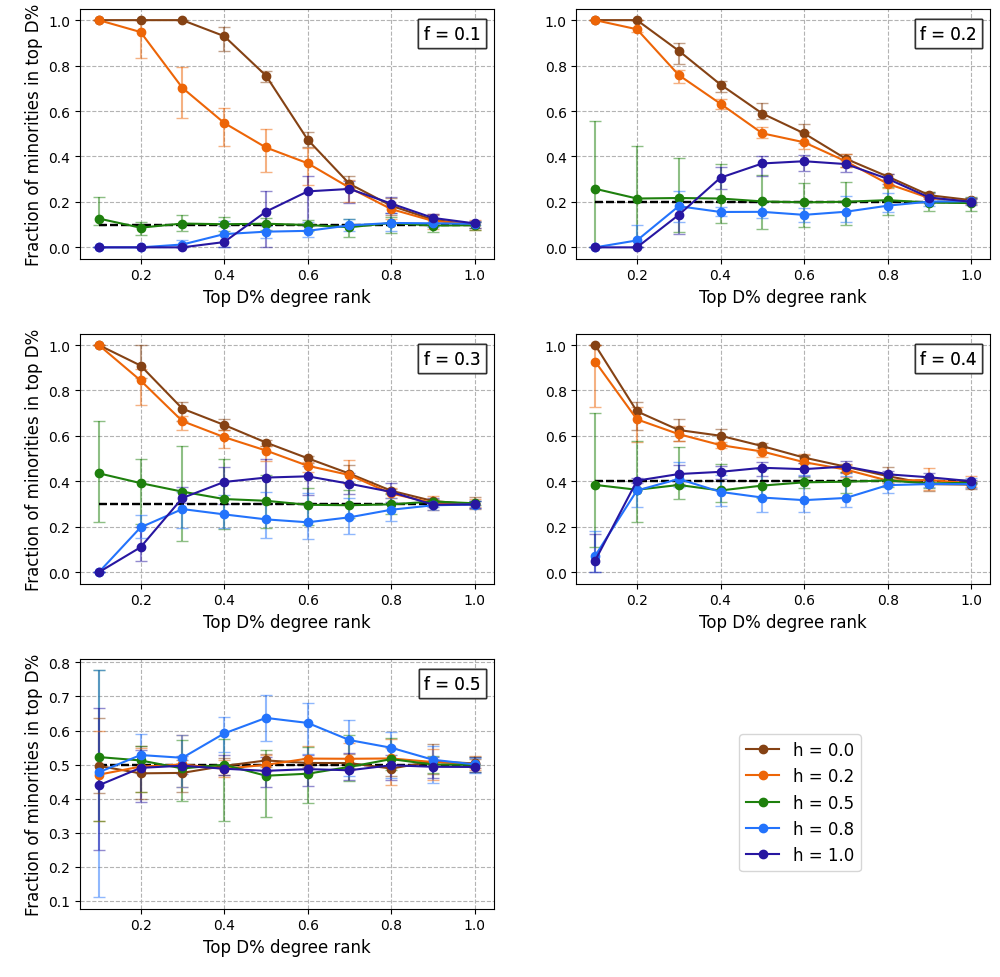
\includegraphics[trim=0 10 0 5, clip, width=1.0\textwidth]{images/top_growth_rb05.png}
	\caption{The fraction of minority nodes found in top D\% nodes ranked according to degree in growing networks with \textbf{Ranked-Bandit ($r = 0.5$)}. A black dotted line at each plot shows the actual fraction of minority nodes in the network.}
	\label{top_growth_rb05_fig}
\end{figure}

%\section{Experimental Results : Ranked-Bandit (r=1.0)}

\begin{figure}[h!]
	\centering
	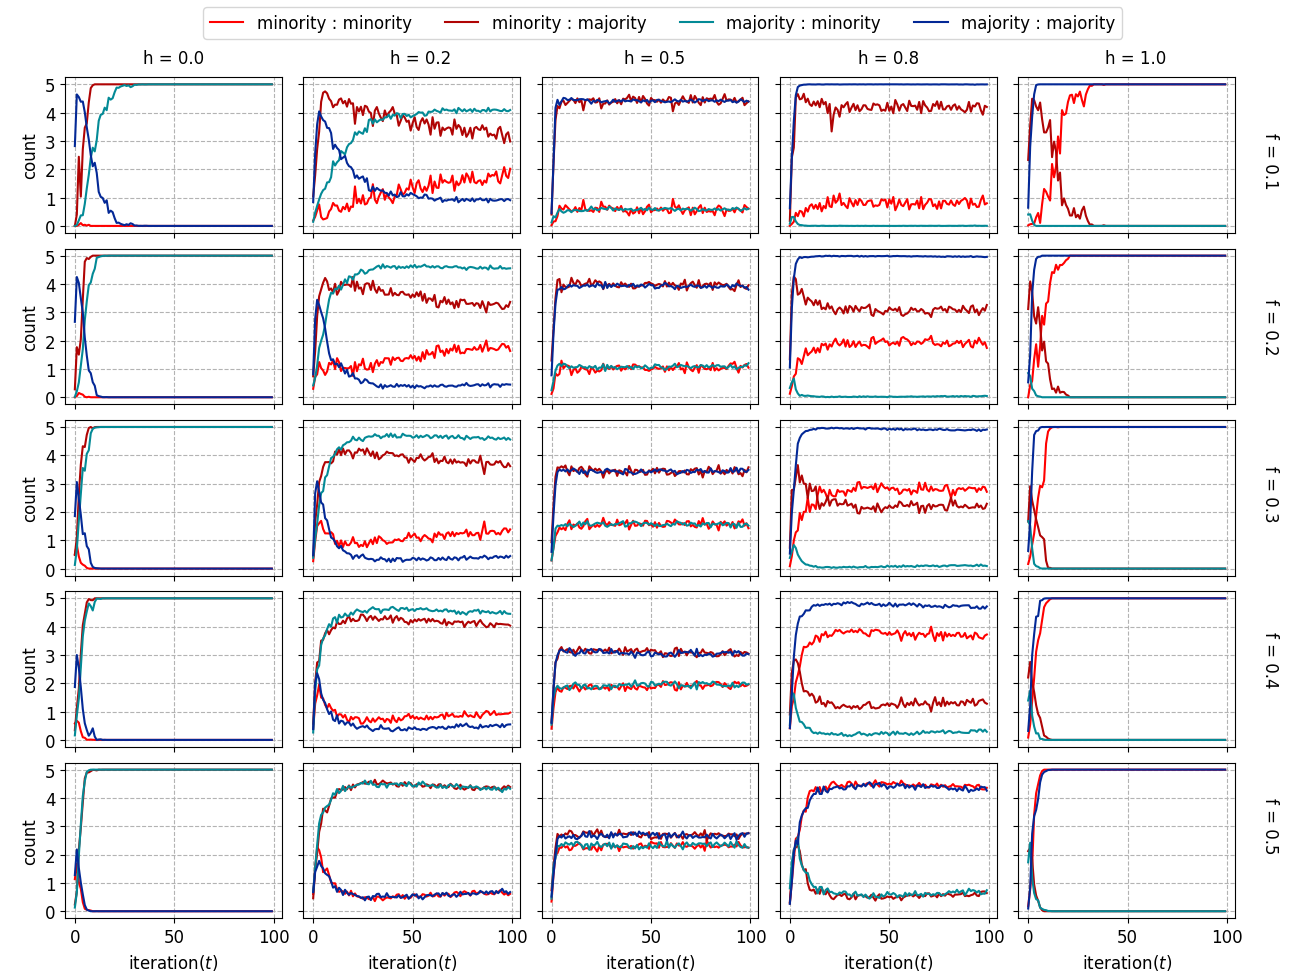
\includegraphics[width=1.0\textwidth]{images/count_rb10.png}
	\caption{Count of nodes in the recommendation list over time for minority and majority nodes in a growing network aided with \textbf{Ranked-Bandit}(r=1.0) recommender agent. Homophily values are specified above the respective columns and minority fractions are specified at the right side of the row. Light red plot line denotes count of minority nodes recommended for other minority nodes. Dark red plot line denotes count of majority nodes recommended for other minority nodes. Light blue line denotes count of minority nodes recommended for other majority nodes. Dark blue line denotes count of majority nodes recommended for other majority nodes.}
	\label{count_rb10}
\end{figure}

%\section{Experimental Results : Top-Rank (r=0.0)}

\begin{figure}[h!]
	\centering
	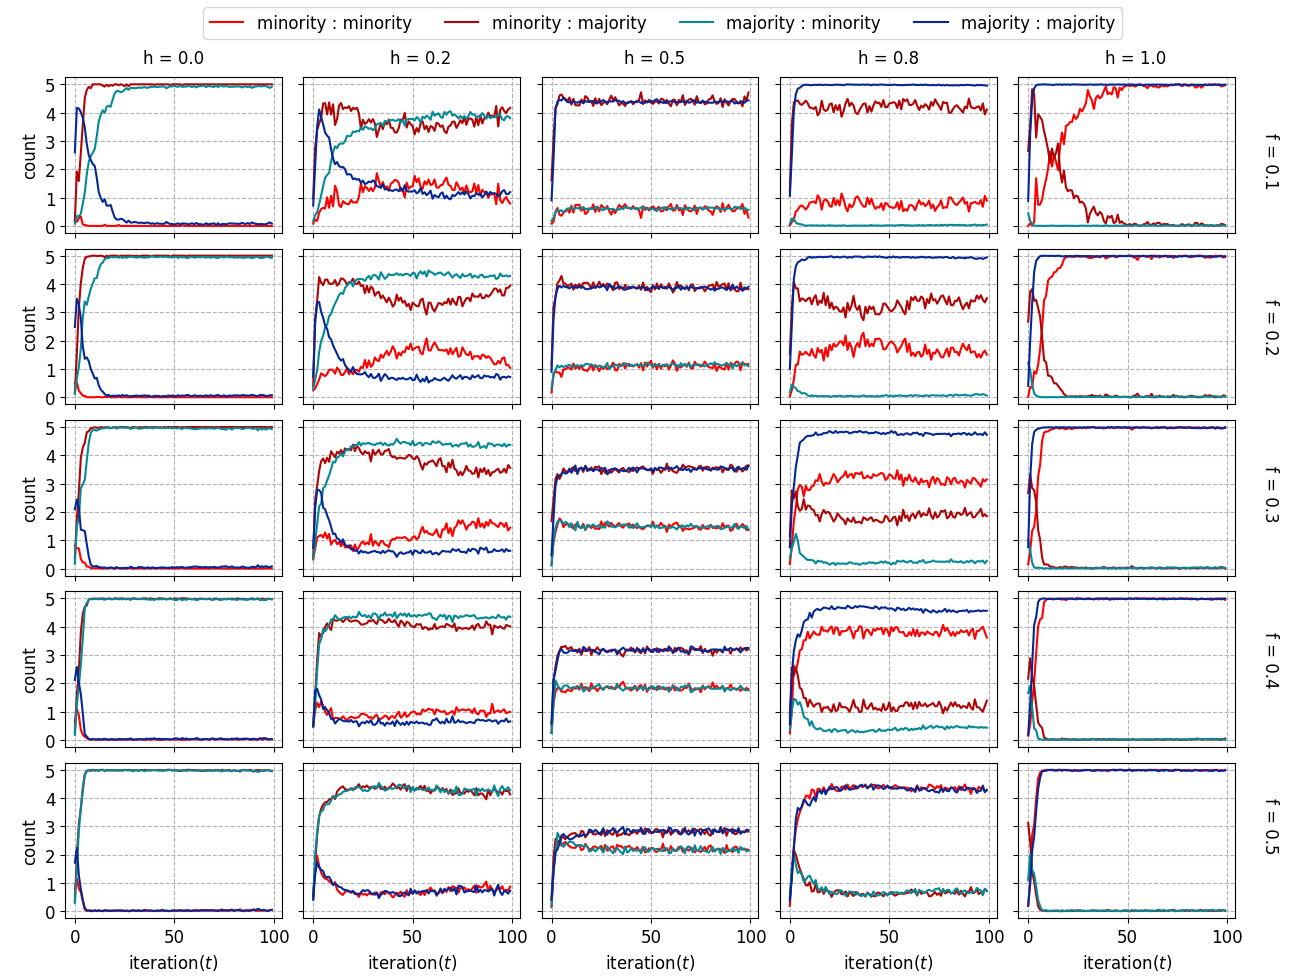
\includegraphics[width=1.0\textwidth]{images/count_top00.png}
	\caption{Count of nodes in the recommendation list over time for minority and majority nodes in a growing network aided with \textbf{Top-Rank}(r=0.0) recommender agent. Homophily values are specified above the respective columns and minority fractions are specified at the right side of the row. Light red plot line denotes count of minority nodes recommended for other minority nodes. Dark red plot line denotes count of majority nodes recommended for other minority nodes. Light blue line denotes count of minority nodes recommended for other majority nodes. Dark blue line denotes count of majority nodes recommended for other majority nodes.}
	\label{count_top00}
\end{figure}

\begin{figure}[h!]
	\centering
	\includegraphics[width=1.0\textwidth]{images/dd_growth_top00.png}
	\caption{Degree distribution for growing networks with \textbf{Top-Rank ($r = 0.0$)}. The minority fractions are provided at the right-side of each row and the homophily values are specified at the top of each column. Degree distribution for the majority and minority nodes are visualized using blue and red plot points respectively.}
	\label{dd_growth_top00_fig}
\end{figure}

\begin{figure}[h!]
	\centering
	\includegraphics[width=1.0\textwidth]{images/dg_growth_top00.png}
	\caption{Degree growth for growing networks with \textbf{Top-Rank ($r = 0.0$)}. The minority fractions are provided at the right-side of each row and the homophily values are specified at the top of each column. Degree growth for minority and majority node is visualized using red and blue color plot lines respectively.}
	\label{dg_growth_top00_fig}
\end{figure}

\begin{SCfigure}[1][h!]
	\centering
	\includegraphics[trim=0 5 0 10, clip, width=0.75\textwidth]{images/mf_growth_top00.png}
	\caption{The fraction of total degree held by minority nodes for growing networks with \textbf{Top-Rank ($r = 0.0$)}.}
	\label{mf_growth_top00_fig}
\end{SCfigure}

\begin{figure}[h!]
	\centering
	\includegraphics[trim=0 10 0 5, clip, width=1.0\textwidth]{images/top_growth_top00.png}
	\caption{The fraction of minority nodes found in top D\% nodes ranked according to degree in growing networks with \textbf{Top-Rank ($r = 0.0$)}. A black dotted line at each plot shows the actual fraction of minority nodes in the network.}
	\label{top_growth_top00_fig}
\end{figure}

%\section{Experimental Results : Top-Rank (r=0.5)}

\begin{figure}[h!]
	\centering
	\includegraphics[width=1.0\textwidth]{images/count_top05.png}
	\caption{Count of nodes in the recommendation list over time for minority and majority nodes in a growing network aided with \textbf{Top-Rank}(r=0.5) recommender agent. Homophily values are specified above the respective columns and minority fractions are specified at the right side of the row. Light red plot line denotes count of minority nodes recommended for other minority nodes. Dark red plot line denotes count of majority nodes recommended for other minority nodes. Light blue line denotes count of minority nodes recommended for other majority nodes. Dark blue line denotes count of majority nodes recommended for other majority nodes.}
	\label{count_top05}
\end{figure}

\begin{figure}[h!]
	\centering
	\includegraphics[width=1.0\textwidth]{images/dd_growth_top05.png}
	\caption{Degree distribution for growing networks with \textbf{Top-Rank ($r = 0.5$)}. The minority fractions are provided at the right-side of each row and the homophily values are specified at the top of each column. Degree distribution for the majority and minority nodes are visualized using blue and red plot points respectively.}
	\label{dd_growth_top05_fig}
\end{figure}

\begin{figure}[h!]
	\centering
	\includegraphics[width=1.0\textwidth]{images/dg_growth_top05.png}
	\caption{Degree growth for growing networks with \textbf{Top-Rank ($r = 0.5$)}. The minority fractions are provided at the right-side of each row and the homophily values are specified at the top of each column. Degree growth for minority and majority node is visualized using red and blue color plot lines respectively.}
	\label{dg_growth_top05_fig}
\end{figure}

\begin{SCfigure}[1][h!]
	\centering
	\includegraphics[trim=0 5 0 10, clip, width=0.75\textwidth]{images/mf_growth_top05.png}
	\caption{The fraction of total degree held by minority nodes for growing networks with \textbf{Top-Rank ($r = 0.5$)}.}
	\label{mf_growth_top05_fig}
\end{SCfigure}

\begin{figure}[h!]
	\centering
	\includegraphics[trim=0 10 0 5, clip, width=1.0\textwidth]{images/top_growth_top05.png}
	\caption{The fraction of minority nodes found in top D\% nodes ranked according to degree in growing networks with \textbf{Top-Rank ($r = 0.5$)}. A black dotted line at each plot shows the actual fraction of minority nodes in the network.}
	\label{top_growth_top05_fig}
\end{figure}

%\section{Experimental Results : Top-Rank (r=1.0)}

\begin{figure}[h!]
	\centering
	\includegraphics[width=1.0\textwidth]{images/count_top10.png}
	\caption{Count of nodes in the recommendation list over time for minority and majority nodes in a growing network aided with \textbf{Top-Rank}(r=1.0) recommender agent. Homophily values are specified above the respective columns and minority fractions are specified at the right side of the row. Light red plot line denotes count of minority nodes recommended for other minority nodes. Dark red plot line denotes count of majority nodes recommended for other minority nodes. Light blue line denotes count of minority nodes recommended for other majority nodes. Dark blue line denotes count of majority nodes recommended for other majority nodes.}
	\label{count_top10}
\end{figure}

\end{appendices}

\end{document}  